% $Id: refman.tex,v 1.50 2009-03-02 10:19:30 weis Exp $

\documentclass[11pt]{report}
\usepackage[english]{babel}
\usepackage{times}
\usepackage[latin1]{inputenc}
\usepackage{fullpage}
\usepackage{color}
\usepackage{listings}
\usepackage{index}
\usepackage{graphicx}

\def\month{August}
\def\year{2009}
\def{\focalversion}{{\sf 0.1.5}}

\def{\focalversiondate}{{\sf {\month} {\year}}}

\newenvironment{citemize}{\begin{list}{$\bullet$}{\itemsep 0pt \topsep 5pt}}{\end{list}}

\def\bbbn{{\rm I\!N}}

\def\url#1{{#1}}
\def\email#1{{\tt#1}}
\def\ocaml{{\sf OCaml}}
\def\moca{{\sf Moca}}
\def\focal{{\sf FoCaLiZe}}
\def\coq{{\sf Coq}}
\def\cime{{\sf CiME}}
\def\zenon{{\sf Zenon}}
\def\zvtov{{\sf zvtov}}
\def\focdoc{{\sf FoCaLiZeDoc}}
\def\dotty{{\sf dotty}}
\def\graphviz{{\sf graphviz}}
\def\emacs{{\sf emacs}}
\def\cygwin{{\sf Cygwin}}
\def\xsltproc{{\sf xsltproc}}
\def\terminal#1{\mbox{\tt\color{red}#1}}
\def\foc{{\sf Foc}}
\def\oldfocal{{\sf Focal}}
\def\focalizec{{\sf focalizec}}

\def\backslash{{\char92}}
\def\chapeau{{\char94}}
\def\vertical{{\char124}}
\def\tilde{{\char126}}

%% Pour afficher les listings de mani�re plus sexy... ;)
\lstdefinelanguage{FoCaLiZe}
  {morekeywords={alias, all, and, as, assume, assumed, begin, by, caml,
      collection, coq, coq_require, definition, else, end,
      ex, external, false, function, hypothesis, if, in,
      inherit, internal, implement, is, let, lexicographic,
      local, logical, match, measure, not, notation, of, open,
      on, or, order, proof, prop, property, prove, qed, rec,
      representation, Self, signature, species, step,
      structural, termination, then, theorem, true, type, use,
      with, conclude},
    otherkeywords={->, :, /\\, \\/, =>, \~, \#, ;, \&, \|},
    sensitive=false,
    morecomment=[n]{(*}{*)},  %% Autoriser les nested comments
    morecomment=[n]{(**}{*)}, %% Autoriser les nested comments
    morestring=[b]",
  }

\lstset{
  language=FoCaLiZe, tabsize=2, frame=single, breaklines=true,
  basicstyle=\ttfamily, framexleftmargin=1mm, xleftmargin=1mm
}

% For syntax definitions
% \begin{syntax}
% left-hand side & ::=  & right-hand side & comment \\
%                & \alt & more right-hand side & more comment
% \end{syntax}
% Use \syntaxclass{Foo} to insert a title line above a syntax definition.
% Do not put \\ before \end{syntax} or \syntaxclass{...}
% Use \begin{syntaxleft} ... \end{syntaxleft} to insert the title
% lines to the left of the definitions.

% \def\syntax{
% \par\medskip\goodbreak\noindent
% \bgroup
% \let\\=\cr
% \interlinepenalty=50            % discourage page breaks in a definition
% \global\let\syntaxclass=\firstsyntaxclass
% \if@twocolumn
% \halign\bgroup~~$##$&\hfil${}##{}$&$##$~\hfil&##\hfil\cr
% \else
% \halign\bgroup\qquad\qquad$##$&\hfil${}##{}$&$##$\quad\hfil&##\hfil\cr
% \fi
% }
% \def\endsyntax{\cr\egroup\egroup\par\medskip\noindent\ignorespaces}

% \def\firstsyntaxclass#1{
% \omit\hbox to 0pt{#1\hss}\cr
% \global\let\syntaxclass=\nextsyntaxclass
% }

% \def\nextsyntaxclass#1{
% \cr\noalign{\smallskip\penalty-100}\omit\hbox to 0pt{#1\hss}\cr
% }

% \def\syntaxleft{
% \par\medskip\goodbreak\noindent
% \bgroup
% \let\\=\cr
% \interlinepenalty=50            % discourage page breaks in a definition
% \global\let\syntaxclass=\firstsyntaxclassleft
% \if@twocolumn
% \halign\bgroup\hfil$##$&\hfil${}##{}$&$##$~\hfil&##\hfil\cr
% \else
% \halign\bgroup\hfil$##$&\hfil${}##{}$&$##$\quad\hfil&##\hfil\cr
% \fi
% }
% \let\endsyntaxleft=\endsyntax

% \def\firstsyntaxclassleft#1{
% $\hfilneg#1\quad\hfil$
% \global\let\syntaxclass=\nextsyntaxclassleft
% }

% \def\nextsyntaxclassleft#1{
% \cr\noalign{\smallskip\goodbreak}$\hfilneg#1\quad\hfil$
% }


\makeindex{}

\begin{document}

\vspace*{3cm}

\begin{center}

{\Huge \textbf{\focal}}

%HEVEA\setcounter{cuttingdepth}{0}
%HEVEA\title{The {\focal} system, release {\focalversion}}

\vspace*{3cm}

{\Huge \textbf{Reference Manual}}


\vspace*{2cm}

{\LARGE \textbf{\focalversion} }

\vspace*{1cm}

{\LARGE \textbf{\focalversiondate}}


\vspace*{3cm}


{\Large \textbf{Authors}}

\mbox{} \vspace*{2cm}

{\large\em
%%%% please add your name as soon as you modify the tex - Th-%%%
Th\'er\`ese Hardin,
Fran\c{c}ois Pessaux,
Pierre Weis,
Damien Doligez
}
\end{center}

\newpage

\begin{center}
{\Huge \textbf{About {\focal}}}
\end{center}


\bigskip

{\large\em {\focal} is the result of a collective work of several researchers,
listed in the following, who designed, defined, compiled, studied,  extended,
used and debugged the preceding versions. They were helped by many
students who had a summer internship under their supervision. They
would like to thank all these students and more generally all the
persons who brought some contribution to {\focal}. }


\vspace*{2cm}

\begin{center}
{\Large \textbf{ {\focal} contributors}}
\mbox{} \vspace*{2cm}
\end{center}


{\large Philippe Ayrault (SPI-LIP6), William Bartlett (CPR-CEDRIC), Julien
Blond (SPI-LIP6), Sylvain Boulm\'e (SPI-LIP6), Matthieu Carlier
(CPR-CEDRIC),  Damien Doligez (GALLIUM-INRIA), David Delahaye
(CPR-CEDRIC), Catherine Dubois (CPR-CEDRIC), Jean-Fr\'ed\'eric Etienne
(CPR-CEDRIC), St\'ephane Fechter (SPI-LIP6), Mathieu Jaume (SPI-LIP6),
Lionel Habib (SPI-LIP6), Th\'er\`ese Hardin (SPI-LIP6), Charles
Morisset (SPI-LIP6), Ivan Noyer (SPI-LIP6), Fran\c{c}ois Pessaux
(SPI-LIP6), Virgile Prevosto (SPI-LIP6), Renaud Rioboo (CPR-CEDRC),
Lien Tran (SPI-LIP6), V\'eronique Vigui\'e Donzeau-Gouge (CPR-CNAM),
Pierre Weis (ESTIME-INRIA)}

\bigskip

\begin{center}
{\large \textbf{and their institutions}}
\mbox{} \vspace*{2cm}
\end{center}

{\em SPI (Semantics, Proofs and Implementations) is a team of LIP6,
(Laboratoire d'Infor\-matique de Paris 6) of UPMC (Pierre and Marie Curie
University)\footnote{UPMC-LIP6,
104 avenue du Pr\'esident Kennedy, Paris 75016, France,
\email{Firstname.Lastname@lip6.fr}}.}

\bigskip


{\em CPR (Conception et Programmation Raisonn\'ees) is a team of CEDRIC
(Centre d'Etudes et de Recherches du CNAM) of CNAM (Conservatoire National
des Arts et M\'etiers)\footnote{CNAM-CEDRIC,
292 rue Saint Martin, 75003, Paris, France,
\email{Firstname.Lastname@cnam.fr}} and ENSIIE (Ecole Nationale d'Informatique pour
l'Industrie et l'Entreprise)\footnote{ENSIIE-CEDRIC,
1 Square de la R\'esistance, 91025 Evry Cedex, France,
\email{Lastname@ensiie.fr}}. }

\bigskip
{\em
ESTIME and GALLIUM are teams of INRIA Rocquencourt\footnote{INRIA,
  Bat 8. Domaine de Voluceau, Rocquencourt, BP 105, F-78153 Le
  Chesnay, France, \email{Firstname.Lastname@inria.fr}}
}


\bigskip

\bigskip


\begin{center}
{\Large \textbf{Thanks}}
\mbox{} \vspace*{2cm}
\end{center}

The {\foc} project was first partially supported by LIP6 (Projet Foc, LIP6
1997) then by the Ministry of Research (Action Modulogic).
The {\oldfocal} research team was then partially supported by the French SSURF ANR project
ANR-06-SETI-016 (Safety and Security UndeR Focal). The project also
benefited of strong collaborations with EDEMOI ANR project and with
BERTIN and SAFERIVER companies.

The {\focalize} language and compiler development effort started around 2005.
The architecture conception and code rewritting started from scratch in 2006
to finally make the first focalizec compiler and {\focalize} system
distribution in 2009, January.

This manual documents the completely revised system with the new syntax and
its semantics extensions.

%%%%%%%%%%%%%%%%%%%%%%%%%%%%%%%%%%%%%%%%%%%%%%%%%%%%%%%%%%%%%%%%%%%%%%%
\setcounter{tocdepth}{5}
\setcounter{secnumdepth}{5}
\tableofcontents


%%%%%%%%%%%%%%%%%%%%%%%%%%%%%%%%%%%%%%%%%%%%%%%%%%%%%%%%%%%%%%%%%%%%%%%
%%%%%%%%%%%%%%%%%%%%%%%%%%%%%%%%%%%%%%%%%%%%%%%%%%%%%%%%%%%%%%%%%%%%%%%
%%%%%%%%%%%%%%%%%%%%%%%%%%%%%%%%%%%%%%%%%%%%%%%%%%%%%%%%%%%%%%%%%%%%%%%

\newpage

\section*{Introduction}

%%%% Intro to give a short description of motivations and milestones
%%%% in the development.
% $Id: motivations.tex,v 1.12 2009-09-02 17:18:23 weis Exp $


\subsection*{Motivations}

The {\foc} project was launched in 1998 by T. Hardin and R. Rioboo
\cite{HardinRiobooTSI04} \footnote{They were members of the SPI (Semantics, Proofs,
Implementations) team of the LIP6 (Lab. Informatique de Paris 6)
at Universit\'e Pierre et Marie Curie (UMPC), Paris}
with the objective of helping all stages of  development of critical software
within safety and security domains. The  methods used in these domains
are evolving, ad-hoc and empirical approaches  being replaced by more formal
methods. For example, for high levels of safety, formal models of the
requirement/specification phase are more and more considered as they
allow mechanized proofs, test or static analysis of the required
properties.  In the same way, high level assurance in system security asks for
the use of true formal methods along the process of software
development and is often required for the specification level.
Thus  the project was to elaborate an Integrated
Development Environment (IDE) able to provide high-level and justified
confidence to users, but remaining easy to use by well-trained
engineers.

To ease developing high integrity systems with numerous software
components, an IDE should provide
tools to formally express specifications, to describe design and
coding and to ensure that specification requirements are met by the
corresponding code. But this is not enough. First, standards of critical systems
ask for pertinent documentation which has to be maintained along all the revisions
during the system life cycle. Second, the evaluation conformance
process of software is by nature a skeptical analysis. Thus, any proof
of code correctness must be easily redone at request and traceability
must be eased. Third, design
and coding are difficult tasks. Research in software engineering has
demonstrated the help provided by some object-oriented
features as inheritance, late binding and early research works on
programming languages have pointed out the importance of abstraction
mechanisms such as modularity to help invariant preservation. There are
a lot of other points which should also be considered when designing
an IDE for safe and/or secure systems to ensure conformance with high
Evaluation Assurance or Safety Integrity Levels (EAL-5 to 7 or SIL 3 and 4)
and to ease the evaluation process according to various standards
(e.g. IEC61508, CC, ...): handling of non-functional contents of
specification, handling of dysfunctional behaviors and vulnerabilities
from the true beginning of development as well as fault avoidance and fault
detection by validation testing, vulnerability and safety analysis.


\subsection*{Initial application testbed}

 When the {\foc} project was launched by T. Hardin and R. Rioboo,
only the specific domain of Computer Algebra was initially considered.
Algorithms used in this domain can be rather intricated and
difficult to test and this is not rare that computer algebra systems
issue a bad result, due to semantical flaws, compiler anomalies,
etc. Thus the idea was to design a language allowing to specify the
mathematics underlying these algorithms and to go step by step to
different kinds of implementations according to the specifities of the
problem under consideration\footnote{For example Computer Algebra
Libraries use different representations of polynomials
according to the treatment to be done}. The first step was to design
the semantics of such a language, trying to fit to several
requirements: easing the expression of mathematical statements, clear
distinction between the mathematical structure (semi-ring, polynomial,
..)  and its different implementations, easing the development
(modularity, inheritance, parametrisation, abstraction, ..), runtime
efficiency and confidence in the whole development (mechanised proofs,
..).  After an initial phase of conceptual design, the {\foc}
semantics was submitted to a double test. On one hand, this semantics
was specified in {\coq} and in a categorical model of type theories by
S. Boulm\'e (see his thesis \cite{BoulmePhD00}), a point which
enlightened the borders of this approach, regarding the logical % [EJ] pas compris "border" -> "limits" ?
background. On the other hand, as a preliminary step before designing the syntax,
a strudy of the typical development style was conducted.
R. Rioboo~\cite{ThRRCalculemus,HardinRiobooTSI04} used the
{\ocaml} language to try different solutions, recorded in
~\cite{HardinRiobooTSI04}.

\subsection*{Initial {\oldfocal} design}

Then the time came to design the syntax of the language and the compiler. To
overcome inconsistencies risks, an original dependency analysis was
incorporated into the compiler (V. Prevosto
thesis \cite{PrevostoPhD03,TPHOL2002,PrevostoJAR02}) and the correction of the
compiler (mostly written by V. Prevosto) against {\oldfocal}'s semantics is
proved (by hand) \cite{TLCA2005}, a point which
brings a satisfactory confidence in the language's correctness. Then
R. Rioboo\cite{BHR2} began the development of a huge Computer Algebra
library, offering full specification
and implementation of usual algebraic structures up to multivariate
polynomial rings with complex algorithms, to
extensively test the language and the
efficiency  of the produced code, aswell as to provide a standard library
of mathematical backgrounds. D. Doligez \cite{ZenonBDD} started the
development of {\zenon}, an automatic prover based on tableaux method,
which takes a {\oldfocal} statement and tries to build a proof of it and,
when succeeds,  issues a {\coq} term. More  recently, M. Carlier and
C. Dubois\cite{CarlierDuboisLNCS2008} began the development of a
test tool for {\oldfocal}.

{\oldfocal} has already been used to develop huge examples such as  the
standard library and the computer algebra library. The library
dedicated to the algebra of access control models, developed by
M. Jaume and C. Morisset \cite{jias06,fcsarspa06,MorissetPhd},
is another huge example, which borrows implementations of orderings,
lattices and boolean algebras from the computer algebra library.
{\oldfocal} was also very successfully used to formalize airport security
regulations, a work by D. Delahaye, J.-F. Etienne, C.  Dubois,
V. Donzeau-Gouge ~\cite{EDEMOI-All,EDEMOI-Model,EDEMOI-Proof}. This
last work led to the development of a translator \cite{Focal-UML}
from {\oldfocal} to UML for documentation purposes.

\subsection*{The {\focal} system}

The {\focal} development started in 2006, as a
continuation of the {\foc} and {\oldfocal} efforts. The new system was rewritten
from scratch. A new language and syntax was designed and carefully
implemented, with in mind ease of use, expressivity, and programmer
friendlyness. The addition of powerful data structure definitions -- together
with the corresponding pattern matching facilities -- leads to new expressive
power.

The {\zenon} automatic theorem prover was also integrated in the
compiler and natively interfaced within the {\focal} language. New
developments for a better support of recursive functions is on the way (in particular for
termination proofs).



\subsection*{The {\focal} system in short}

The {\focal} system provides means for the developers to formally express
their specifications and to go step by step (in an incremental approach) to
design and implementation while proving that such an implementation
meets its specification or design requirements. The {\focal} language offers
high level mechanisms such as multiple inheritance, late binding, redefinition,
parametrization, etc.  Confidence in proofs submitted by developers or
automatically done relies on formal proof verification. {\focal} also
provides some automation of documentation production and management.

A formal specification can be built by declaring names of functions
and values and introducing
properties. Then, design and implementation can incrementally be done
by adding definitions of functions and proving that the implementation
meets the specification or design requirements. Thus, developing in
{\focal} is a kind of refinement process from  formal model to design
and code, completely done within {\focal}. Taking the global development
in consideration within the same environment brings some conciseness,
helps documentation and reviewing.

A {\focal} development is organised as a hierarchy that may have
several roots. The upper levels of the hierarchy are built along the
specification stage while the lower ones correspond to
implementation and each  node of the hierarchy corresponds to a progress
toward a complete implementation.

We would like to mention several works about safety and/or security
concerns within {\focal} and specially the definition of a safety life
cycle by P. Ayrault, T. Hardin and F. Pessaux \cite{TTSS08} and the
study of some traps within formal methods by E. Jaeger and
T. Hardin\cite{traps}.

{\focal} can be seen as an IDE still in development, which
gives a positive solution to the three requirements identified above:

\begin{enumerate}
\item pertinent documentation is maintained within the system being written,
      and its extraction is an automatic part of the compilation process,
\item proofs are produced using an automated proved which can be guided using a high level proof language, so that proofs
      are easier to write and their verification is automatic and reliable,
\item the framework provides powerful abstraction mechanisms to facilitate
      design and development; however, these mechanisms are carefully ruled:
      the compiler performs numerous validity checks to ensure that no
      further development can inadvertantly break the invariants or
      invalidate the proofs; indeed, the compiler ensures that if a theorem
      was based on assumptions that are now violated by the new development,
      then the theorem is out of reach of the programmer and the properties have to be proven again.
\end{enumerate}







%%%%%%%%%%%%%%%%%%%%%%%%%%%%%%%%%%%%%%%%%%%%%%%%%%%%%%%%%%%%%%%%%%%%%%%
%%%%%%%%%%%%%%%%%%%%%%%%%%%%%%%%%%%%%%%%%%%%%%%%%%%%%%%%%%%%%%%%%%%%%%%
%%%%%%%%%%%%%%%%%%%%%%%%%%%%%%%%%%%%%%%%%%%%%%%%%%%%%%%%%%%%%%%%%%%%%%%
\chapter{Overview}
%%%% a smooth introduction to focal main concepts before entering the
%%%% true reference manual.

% $Id: glimpse.tex,v 1.14 2009-08-25 12:38:07 weis Exp $
\def\bbbn{{\rm I\!N}} % [EJ] Sinon il y a \mathbb{N} qui fait �a bien aussi...
\label{glimpse}
Before entering the precise description of {\focal}, we give an
informal presentation of its main features, to help further reading of the
reference manual. Every construction or feature that we sketch here is
entirely and precisely described in the following chapters.

\section{The Basic Brick}

The primitive entity of a {\focal} development is the
{\em species}. It can be viewed as a record grouping ``things'' related
to the same concept. Like in most modular design systems (i.e. objected
oriented, algebraic abstract types), the idea is to group a data
structure with the operations that operate on it. Since in {\focal} we don't
only address data type and operations, these ``things'' also
comprise the declaration (or specification) of the operations,  their
stated properties (which represent the requirements for the operations), and the
proofs of these properties.

We now informely describe each of these ``things'', called the {\em methods}
of the species.

\begin{itemize}
  \item The
    {\tt representation} gives the data representation of the entities
    manipulated by the {\em species}. It is a type
    defined by a type expression.
    The {\em representation} definition may be deferred,
    which means that the structure of the embedded data-type
    does not  need to be known at this point. In this case, it is
    simply a type variable.  However, to finally obtain an
    implementation,  the {\em representation}
    has to be defined at some point, either by setting
    {\tt representation = type\_exp} where {\tt  type\_exp} is a type
    expression or by inheritance (see below).
    Type expressions in {\focal} are roughly speaking the ML type expressions (variables,
    basic types, inductive types, record types).
%     {\em species representation types}, denoted by keyword {\tt Self}
%     inside the species and by  the name of their {\em species}
%     outside of them.

    Each {\em species} has a unique {\em representation}. This
    is not a restriction compared to other languages where
    programs/objects/modules can own several private variables
    representing the internal state, since the variables define some part of
    the data structure of the entities manipulated by the
    program/object/module.
    The equivalent {\focal} {\em representation} is simply a tuple grouping
    in one place all these variables that were disseminated in the entire
    program/object/module.


  \item Declarations are composed of the keyword {\tt signature}
    followed by a name and a type. They announce a {\em method} to
    be defined later (the type of the method is given but the implementation
    is still omitted).
%    for specification or design purposes since declared names may be
%    used  to define others {\em methods} while
    Once a method is declared, this method can be used in the text following
    the declaration, in particular in the definition of other methods:
    indeed, the type provided by the {\em signature} allows the {\focal} compiler to check
    that the method is consistently used in all contexts with a type compatible with the
    declared type. Furthermore, the late-binding and the collection mechanisms
    introduced below, ensure that the definition of the method is
    known when the method is effectively invoked.

  \item Definitions are composed of the keyword {\tt let}, followed
    by a name, an optional type, and an expression. They serve to introduce
    constants or functions, i.e. computational operations. The core
    language used to implement them is roughly ML-like expressions
    (let-binding, pattern matching, conditional, higher order
    functions, \ldots) with the addition of a construction to call a
    {\em method} from a given {\em species}. Mutually recursive
    definitions are introduced by {\tt let rec}.



  \item Property statements are composed of the keyword {\tt property}
    followed by the name of the property and its definition, a first-order formula.
    A {\em property} may serve to express requirements
    (i.e. a fact that the system must hold to conform to the Statement
    of Work) and in this case we can view the property as a
    specification purpose {\em method}, like a {\em signature} was for
    {\tt let}-{\em method}s. A property induces a {\em proof obligation} to
    be discharged at some point in the development. A {\em property} may also
    be used to express some ``quality'' information of the system (soundness,
    correctness, \ldots) also submitted to a proof obligation.
    The formulae % [EJ] Pas compris quality information
    are written with the usual logical connectors, universal and
    existential quantifications over a {\focal} type, and cite the name of
    any {\em method} known within the {\em species}' context. For instance,
    a {\em property} telling that for any vehicle, if the speed is non-null,
    then the doors cannot be opened could look like:
    \begin{center}
    {\tt all m in Self, !speed(m) <> Speed!zero -> \tilde doors\_open(m)}
    \end{center}
    In the same way as {\em signatures}, a yet to be proved {\em property}
    can be used as an hypothesis in the proof of other properties or
    theorems.
    Once more, the {\focal} late binding and collection mechanisms ensure
    that the proof of a {\em property} will be ultimately done.

  \item Theorems ({\tt theorem}) made of a  name, a statement and a
    proof are {\em properties} packed with the formal proof that their
    statement holds in the context of the {\em species}. The proof
    accompanying the statement will be processed by {\focal}, {\zenon} and
    ultimately checked with the {\coq} theorem prover.

\end{itemize}

Regarding properties and theorems, note that like in any formal development,
the difficulty may be more to express a true, interesting and meaningful
statement, than to prove it. For instance, claiming that a piece of software
is ``formally proved'' because it respects a safety requirement is
meaningless if the statement of this requirement is trivially true
(see \cite{traps} for examples).
%      system\_ok}. This is obviously a non-sense since the text of the
%    property is trivial and does not link {\tt system\_ok} with the
%    rest of the software (see \cite{traps} for less trivial examples).

Let's illustrate these notions on an example that we incrementally
extend. We want to model some simple algebraic structures. Let's start
with the description of a ``setoid'' representing the data structure of
``things'' belonging to a set, which can be submitted to an
equality test and exhibited (i.e. one can get a witness of existence of one
of these ``things'').

{\scriptsize
\begin{lstlisting}
species Setoid =
  signature ( = ) : Self -> Self -> bool ;
  signature element : Self ;

  property refl : all x in Self, x = x ;
  property symm : all x y in Self, x = y -> y = x ;
  property trans: all x y z in Self, x=y and y=z -> x=z ;
  let different (x, y) = basics#not_b (x = y) ;
  theorem different_irrefl : all x in Self, ~different(x, x)
   proof = by definition of different
              property refl ;
end ;;
\end{lstlisting}
}

In this {\em species},  the {\em representation} is not explicitly
given (the keyword {\tt representation} is not used), since we don't need to set
it to the express functions and properties that a ``setoid''
requires. However, we can refer to the representation via {\tt Self}
(in this case a type variable). In the same way, we just specify a {\em
signature} for the equality (operator {\tt =}). We introduce the three
properties that the equality must have (exactly the properties of an equivalence
relation).

We complete the example by the definition of
the function {\tt different} which uses the (not yet defined) {\tt =} method,
and the predefined boolean negation {\tt basics\#not\_b}.

Not only we can define {\tt different} out of a not yet defined method {\tt
=}, we can also prove a property of {\tt different} based on
the not yet proved properties of {\tt =}! Indeed we prove that
{\tt different} is irreflexive, under the hypothesis that {\tt =} is an
equivalence relation (i.e. that any implementation of {\tt =} used by
{\tt different} will satisfy these properties).

Note: {\tt basics\#not\_b} stands for the function {\tt not\_b} defined in
the {\focal} {\tt basics} development (which is in the source file {\tt
basics.fcl} of the standard library).

\bigskip

In {\focal}, the {\em late-binding} feature makes it possible to use {\em
methods} as soon as they have been declared and way before they get a
real {\em definition}. Similarly, {\focal} allows arbitrary {\em method}
redefinition: the effective {\em definition} of the method
inside a species is guarrantied to be the last version of the successive
definitions of the method.

\section{Type of Species, Interfaces and Collections}
\label{species-type}
\label{species-interface}
The {\em type} of a {\em species} is obtained by removing all the definitions
and proofs. Thus, it is somoe kind of record type, made of all the method
types of the species. If the {\tt representation} is still a type
variable say $\alpha$, then the {\em species} type is prefixed with an
existential binder $\exists \alpha$. This binder is eliminated as
soon as the {\tt representation} is known.
Technically, the existancial type variable is instantiated when the
representation type is defined; furthermore, the compiler checks that
all existancial type variables have been eliminated before the generation of
runnable code.

\bigskip

The {\em interface} of a species is obtained by abstracting the {\em
representation} type in the {\em species type}; this abstraction
is permanent.

\bigskip

{\bf Warning} {\em  No special construction
is given to denote the interface of a species in the concrete syntax,
it is simply denoted by the name of the species.} Do not
confuse a species and its interface.

\bigskip

The {\em species type} remain totally implicit in the concrete syntax, being
just used as a step to build the {\em species interface}. It is used
during inheritance resolution.

Interfaces can be ordered by inclusion, a point providing a very
simple notion of subtyping. This point will be further commented.


A species is said to be {\em complete} when the representation and all the
declarations have received a definition and all the properties have received
a proof.

When {\em complete}, a species can be submitted to an abstraction process of
its representation to create a {\em collection}. Put it the other way round:
a collection abstracts a complete species. Thus, the {\em interface} of a
collection is the {\em interface} of the abstracted complete species. Thus, a
collection is a kind of abstract data type, only usable through
the methods of its interface, with the addional guarantee that all the
declarations have been defined and all the statements have been proved.


\section{Combining Bricks by Inheritance}

A {\focal} development is organised as a hierarchy which may have
several roots. Usually the upper levels of the hierarchy are built
during the specification stage while the lower ones correspond to
implementations. Each node of the hierarchy, i.e. each {\em species},
is a progress towards a complete implementation. On the previous
example, putting aside {\tt different},  we typically presented a kind of
{\em species} for ``specification'' since it expresses only
{\em signatures} of functions to be later implemented and properties
to be later proved.

We can now create a new {\em species} by {\bf inheritance} of an already
defined one. We can make this new species more ``complex'' by adding new
operations and properties, or we can make it more concrete by providing
definitions to {\em signatures} and proofs to {\em properties}, without
adding new features.

Hence, the {\focal} inheritance notion serves two kinds of evolutions in the
development process. The first kind of evolution is {\em additional
complexity}: the inheritance makes more complex {\em species} out of simpler
ones; the new species gets more operations than its parents
(keeping the ancestors operations or possibly redefining some of them, if
required).
The second kind of inheritance is {\em refinement}: the new
species has less and less still unknown parts; it tends to the status of a ``runnable''
implementation, providing explicit definitions to the {\em methods} that were
previously only declared.

Continuing our example, we want to extend our model to represent
``things'' with a multiplication and a neutral element for this
operation.

{\scriptsize
\begin{lstlisting}
species Monoid =
  inherit Setoid;
  signature ( * ) : Self -> Self -> Self ;
  signature one : Self ;
  let element = one * one ;
end ;;
\end{lstlisting}
}

{\em Monoid} are ``things'' that are {\em Setoids} but also have an operation
{\tt *} and a specific value called {\em one}; besides the new {\em methods}
we also gave a definition to {\tt element}, saying it is the application of
the method {\tt *} to {\tt one} twice, both of them being only {\em
declared}. Here, we used the inheritance in both the presented ways: making a
more complex entity by adding {\em methods} and getting closer to the
implementation by explicitly defining {\tt element}.

{\focal} provides multiple inheritance. For sake of simplicity,
the above example uses simple inheritance. When inheriting the same
{\em method} from more than one parent, the order of parents apparition in the
{\tt inherit} clause serves to determine the chosen {\em method} (only
the latest definition of any method appearing several times in the
list of inherited species is retained).

The {\em type} of a {\em  species} built using inheritance is defined
like for other {\em species}, the {\em method} types being those of the {\em
methods} appearing in the {\em species} after inheritance resolution.

A strong constraint in inheritance is that the type of inherited,
and/or redefined {\em methods} cannot change.  This is required to
ensure consistency of the {\focal} model, hence of the developed
software. More precisely, if the representation is given by a type
expression containing some type variables, then it can be more defined
by instanciation of these variables. In the same way, two signatures
have compatible types if they have a common unifier; thus, roughly
speaking, if they are compatible as ML-like types. For example, if the
representation was not yet defined (thus being still a type variable),
it can be defined by {\tt int}. And if a species $S$ inherits from
$S_1$ and $S2$ a method called $m$, there is no type clash if $S_1 !m$
and $S_2!m$ can be unified, then the method $S!m$ is addigned the most general
unifier of these two types.

In a nutshell, if a species {\em B} inherits from a species {\em A}, the
intuition is that any instance of {\em B} is also an instance of {\em A}.

\section{Combining Bricks by Parameterisation}

As indicated, inheritance is used to enrich or to implement {\em species}.
However, we sometimes need to use a {\em species}, not to take over
its {\em methods}, but rather to use it as an ``ingredient'' to build
a new structure. For instance, a product of setoids is a
new structure, using the previous {\em species} as the ``ingredient''.
Indeed, the structure of a product is not similar to any of its component,
but is build using the structures of its components. A product
can be seen as {\em parameterised} by its two components.
Following this idea, {\focal} allows two flavors of parameterisation.

\subsection{Parameterisation by Collection}

We first introduce the {\em collection parameters}. They are
{\em collections} that the hosting species may use through their
{\em methods} to define its own ones.


A {\em collection parameter} is given a name $C$ and a (species) interface
$I$.  The name $C$ serves to call the {\em methods} declared in
$I$. Intuitively, $C$ will at some stage be implemented by a collection $CE$
whose interface contains the methods of the interface $I$.  Moreover, the
collection and late-binding mechanisms ensure that all methods appearing in
$I$ are indeed implemented (defined for functions, proved for properties) in
$CE$. Thus, no runtime error, due to linkage of libraries, can occur and any
{\em property} or {\em theorem} stated in $I$ can be safely used as an
hypothesis.

Calling a {\em species}'s {\em method} is
done via the ``bang'' notation:
{\tt !meth} or\break{}{\tt Self!meth} for a {\em method} of the current
{\em species} (and in this case, even simpler: {\tt meth}, since the
{\focal} compiler will resolve scoping issues). To call
{\em collection parameters}'s {\em method}, the same notation is used:
{\tt A!element} stands for the {\em method} {\tt element} of the
{\em collection parameter} {\tt A}.


To go on with our example, a product of setoids has two components, hence a
{\em species} for products of setoids has two {\em collection parameters}. It
is itself a setoid (that is, a ``thing'' with an equality), a fact which is
simply recorded via the inheritance mechanism: {\tt inherit Setoid} gives to
{\tt Setoid\_product} all the methods of {\tt Setoid}.

{\scriptsize
\begin{lstlisting}
species Setoid_product (A is Setoid, B is Setoid) =
  inherit Setoid;

  signature fst : Self -> A ;
  signature snd : Self -> B ;
  signature pair : A -> B -> Self ;

  let element = Self!pair(A!element, B!element) ;

  let ( = ) (x, y) = basics#and_b (A!( = )(fst(x), fst(y)),
                                   B!( = )(snd(x), snd(y))) ;
  proof of refl = by definition of ( = )
                     property A!refl, B!refl ;

end ;;
\end{lstlisting}
}

We first declare methods {\tt fst}, {\tt snd} and {\tt pair} to represent the
two projections and the construction of pairs.
Next, we introduce a definition for {\tt element} by building a pair, using
the function  {\tt pair} applied to the method {\tt element} of respectively {\tt A}
and {\tt B}. We also add a definition for {\tt =} of {\tt Setoid\_product},
relying on the methods {\tt =} of {\tt A} and {\tt B}
(which are not yet defined), and we prove that {\tt =} of {\tt Setoid\_product} is
indeed reflexive, upon the hypothesis made on {\tt A!( = )}
and {\tt B!( = )}.  The part of {\focal} used to write proofs will be
shortly presented later, in section \ref{focal-proof-language}.

Such a species can be refined with {\tt representation = A * B}, indicating
that the representation of the product is the Cartesian Product of the
representation of the two parameters. In {\tt A * B}, {\tt *} is the {\focal}
type �constructor of pairs, {\tt A} denotes indeed the representation of the
first {\em collection parameter}, and {\tt B} the one of of the second {\em
collection parameter}.

This way, the {\em species} {\tt Setoid\_product} builds its {\em
methods} relying on those of its {\em collection parameters}. Note the
two different uses of {\tt Setoid} in our {\em species} {\tt
Setoid\_product}, which both inherits of and is parameterised by it.

\bigskip

Why {\em collection parameters} and not simply {\em species parameters}?
There are two reasons. First, effective parameters must provide
definitions/proofs for all the methods of the required interface: this is the
contract. Thus, effective parameters must be {\em complete} species. Then, we
do not want the parameterisation to introduce dependencies on the parameters'
{\em representation} definitions. For example, it is impossible to express ``
if {\tt A!representation} is {\tt int} and {\tt B!representation} is {\tt
bool} then {\tt A * B} is a list of boolean values''. This would dramatically
restrict the possibilities to instantiate parameters since assumptions on the
{\em representation}, possibly used in the parameterised {\em species} to
write its own {\em methods}, could prevent {\em collections} having the right
set of {\em methods} but a different representation to be used as effective
parameters. Such a behaviour would make parameterisation too weak to be
usable. We choose to always hide the {\em representation} of a {\em
collection parameter} to the parameterised hosting {\em species}. Hence the
introduction of the notion of {\em collection}, obtained by abstracting the
representation from a complete species.

\subsection{Parameterisation by Entity (Value)}

Let us imagine we want to make a {\em species} to implement arithmetic on
natural numbers modulo a certain value. In the expression $5 {\tt\ modulo\ }
2\ is\ 1$, both $5$ and $2$ are natural numbers. To be sure that the {\em
species} will consistently work with the same modulo, this last one must be
embedded in the {\em species}. However, the {\em species} itself doesn't rely
on a particular value of the modulo. Hence this value is clearly a {\bf
parameter} of the species, but a parameter for which need its {\bf value},
not only by its {\em representation} and the methods acting on it. Such a
parameter is named an {\em entity parameter}. Being a value, an entity
parameter belongs to some collection, and this collection must also be declared as a {\em
collection parameter} of the species. An entity parameter denotes a
{\em value} having the type of the {\em representation} of its associated
{\em collection parameter}.

As an exemple, let us define a collection {\tt Modulo\_n}. We first define a
{\em species} to represent natural numbers:

{\scriptsize
\begin{lstlisting}
species NatModel =
  signature one : Self ;
  signature inc : Self -> Self ;
  signature modulo : Self -> Self -> Self ;
end ;;
\end{lstlisting}
}

Note that {\tt NatModel} can be later implemented in various ways, using
Peano's integers, machine integers, arbitrary-precision arithmetic (as well
as things that are not really integers, our specification being too
simplistic)\ldots

The {\em species} ``working modulo n\ldots'' now embeds the value of {\tt n}
as an element of a collection for {\tt NatModel}:
{\scriptsize
\begin{lstlisting}
species Modulo_n (Naturals is NatModel, n in Naturals) =
  let job1 (x : Naturals) =
    ... Naturals!modulo (x, n) ... ;
  let job2 (x : Naturals, ...) =
    ... ... Naturals!modulo (x, n) ... ... ;
end ;;
\end{lstlisting}
}
Using the {\em entity parameter} {\tt n}, we ensure that the
{\em species} {\tt Modulo\_n} works for {\em any} value of the
modulo, but will always use the {\em same} value {\tt n} of the modulo
everywhere inside the {\em species}.


\section{The Final Brick}

As briefly introduced in \ref{species-interface}, a {\em species} needs to be
complete to lead to executable code for its functions and checkable proofs
for its theorems. When a {\em species} is complete, it can be turned into a
{\em collection}. Hence, a {\em collection} represents the final stage of the
inheritance tree of a {\em species} and leads to an effective data
representation with executable functions processing it.

For instance, providing that the previous {\em species} {\tt NatModel} has
been refined into a fully-defined species {\tt MachineNativeInt} through
inheritances steps, with a {\em method} {\tt from\_string} allowing to create
the natural representation of a string, we could get a related collection by:

{\scriptsize
\begin{lstlisting}
collection MachineNativeIntegers =
  implement MachineNativeInt;
end ;;
\end{lstlisting}
}

Next, to get a {\em collection} implementing arithmetic modulo $8$, we
can define a {\em collection} for the {\em species} {\tt Modulo\_n}:

{\scriptsize
\begin{lstlisting}
collection Modulo_8 =
  implement Modulo_n
    (MachineNativeIntegers, MachineNativeIntegers!from_string ("8");
end;;
\end{lstlisting}
}

As exemplify here, a species is applied to effective parameters by giving
their values with the same syntax as for parameter passing.

As said before, to ensure modularity and abstraction, the {\em
representation} of a {\em collection} is hidden (as well as its
definitions). It means that any software component using a {\em collection}
will only be able to manipulate its values through the operations ({\em
methods}) that the collection provides via its interface.  As a corollary, no
other software component can possibly break the invariants required by the
internals of a {\em collection}.

\section{Properties, Theorems and  Proofs}
\label{focal-proof-language}

{\focal} not only provides a way to write programs, it also intends to
encompass both the executable model (i.e. program) and the properties that
this model must satisfy. For this reason, some ``special'' fields of the
species only deal with logic instead of specifying purely behavioural aspects
of the program: those logical aspects are {\em theorems}, {\em properties}
and {\em proofs}.

Stating a {\em property} declares that a {\em proof} that the property {\bf
holds} will be given at some stage of the development. The {\em theorems} are
properties for which the {\em proof} is given with the statement. All the proofs must be
done by the developer; the compiler ultimately send them to the {\coq} proof assistant
for verification: all the demonstrations made in {\focal} are automatically
machine checked for consistency by {\coq}.

{\focal} provides several ways to write proofs. The normal and encouraged way
is to use the {\focal}'s proof language to write the proofs.  The {\focal}'s
proof language (or {\em FPL} for short), is a hierarchical proof language
especially designed to give an easy way to vary the grain of the proof, from
rough sketch to fully detailed proof. As in the usual mathematical activity,
the idea is to provide hints and direction for a proof and let the reader
complete the details. Well, don't panic: you will not have to complete the
proofs of all the {\focal} development you may ever read or write! The proofs
in {\focal} do not require a human being to read them and complete their
numerous omitted details! The {\focal} system delegates this burden to a
companion program: the {\zenon} proof finder.

From the hints given in the {\focal} development, {\zenon} attempts to
generate a complete proof and exhibit a {\coq} proof term suitable for
verification. So far so good! But what happens if {\zenon} fails to find the
(complete) proof ? Well, you can consider this failure as a hint that the
given proof was too sketchy: you have to develop it a bit, for instance by
stating and proving some intermediate lemmas or by detailing the proof path!
Once again, this is rather natural and not so far from normal mathematical
activity.

{\zenon} \cite{ZenonBDD,zenon0.4.1} is developed by D. Doligez. It is
a first order theorem prover based on the tableau method incorporating
implementation novelties such as sharing.

The {\focal} programmer gives basic hints to {\zenon} such as: ``prove by definition
of this {\em method}'' (i.e. look inside the body of the method) or ``prove
by this {\em property}'' (i.e. use the logical statement of a {\em theorem}
or {\em property} already proven). This hint mechanism is embedded into the
entire FPL description of the proof into steps stating assumptions (that must
obviously be demonstrated afterwards) in order to prove some lemmas or parts of
the property at hand.

We now give such a demonstration.

{\scriptsize
\begin{lstlisting}
  theorem order_inf_is_infimum : all x y i : Self,
    !order_inf(i, x) -> !order_inf(i, y) ->
      !order_inf(i, !inf(x, y))
    proof =
      <1>1 assume
             x : Self, y : Self, i : Self,
             hypothesis H1 : !order_inf (i, x),
             hypothesis H2 : !order_inf (i, y),
           prove !order_inf (i, !inf (x, y))
        <2>1 prove !equal (i, !inf (!inf (i, x), y))
          by hypothesis H1, H2
             property inf_left_substitution_rule,
               equal_symmetric, equal_transitive
             definition of order_inf
        <2>f qed
          by step <2>1
             property inf_is_associative, equal_transitive
             definition of order_inf
      <1>f conclude
    ;
\end{lstlisting}
}

The important point is that {\zenon} works for the developer: {\bf it
searches and completes the proof} for the developer that no more have to
elaborate the proof completely formally ``from scratch''.

Like all other automatic theorem prover, {\zenon} may fail to find a
demonstration. In this case, {\focal} allows the developer to write verbatim {\coq}
proofs. Comfort of automation is lost in favor of an increase in expressive power:
the entire {\coq} vernacular language is now available to the developer to
write the proof.

Finally, the {\tt assumed} keyword is the ultimate proof backdoor: the proof
is not given and the property is admitted. Obviously, a safe development
should not make a liberal usage of this feature, since {\tt assumed} bypasses
the formal verification of the software's model. However, such a functionality
remains needed for various reasons. For example, a development may be linked
with external code; the properties of the {\focal} code now depends on properties
of the external code; to continue the development as safely as possible, it
is necessary to carefully state the properties that are assumed for the
external code and go on providing properties and proofs about the program:
those proofs will give valuable confidence, even if they only hold if the set
of assumptions for the external code is valid.

% [EJ] L'utilisateur saura quand utiliser assumed, mais l'exemple donne me semble
% inapproprie. En effet, l'exemple x+1>x est justement faux pour les entiers
% machine, et il ne devrait pas etre admis de maniere generique. Ce sera sans doute
% le choix de certains developpeurs de l'admettre, mais c'est hors du scope du manref

\section{Around the Language}

In the previous sections, we presented {\focal} through its programming model
and shortly its syntax. We especially investigated the various entities
making a {\focal} program. We now address what becomes a {\focal} program
once compiled. We recall that {\focal} supports the redefinition of
functions, which permits for example to specialise the code to a specific
representation of data (for example, there exists a generic implementation of
integer addition modulo {\tt n} but this implementation can be redefined in
arithmetics modulo {\tt 2}, if boolean values are used to represent the two
values). {\focal) is also a very convenient tool to maintain software.

\subsection{Consistency of the Software}

All along the {\focal} development cycle, the compiler keeps trace of
dependencies between {\em species}, {\em methods}, and {\em proofs} \ldots to
ensure that all the modifications are consistently propagated to any place
that needs to be changed.

{\focal} deals with two types of dependencies:
\begin{itemize}
\item The {\bf decl}-dependency: a {\em method} $A$ decl-depends on a
  {\em method} $B$, if the {\bf declaration} of $B$ is required to
  state $A$.
\item The {\bf def}-dependency: a {\em method} (and more especially, a
  {\em theorem}) $A$ def-depends on a {\em method} $B$, if the
  {\bf definition} of $B$ is required to state $A$ (and more
  especially, to prove the property stated by the {\em theorem}
  $A$).
\end{itemize}

The redefinition of a function may invalidate the proofs that use the
properties of the body of the function. All the proofs which truly depend of
the definition are then invalidated by the compiler and must be done again in
the updated context where the function gets the new definition. Thus, choose
the proper level in the hierarchy to do a proff is a major practical
difficulty. In \cite{PrevostoJaume2003}, Prevosto and Jaume propose
a \emph{coding style} to minimise the number of proofs to be redone in case
of redefinition, by using a certain kind of modularisation for the proofs.

\subsection{Code Generation}

{\focal} currently compiles programs toward two languages, {\ocaml} to
get an executable standalone, and {\coq} to have a formal model
of the program, with theorems and proofs entirely machine checked.

In the {\ocaml} code generation, all the logical aspects are discarded since
they do not lead to executable code.

In contrast, in {\coq}, all the {\em methods} are compiled,
i.e. ``computational'' {\em methods} and logical {\em methods} with their
proofs. This allows {\coq} to check the entire consistence of the system
developed in {\focal}.


\def\focaltest{FocalTest}

\subsection{Tests}
{\focal} incorporates a tool named {\em \focaltest}
\cite{CarlierDuboisLNCS2008} for Integration/Validation testing. It
allows to confront automatically a property of the specification with an
implementation. It automatically generates test cases, executes them and
produces a test report as an XML document. The property under test is used to
generate the test case but also as an oracle. When a test case fails, it
means that a counterexample of the property has been found: the
implementation does not match the property. This surely points out an
inconsistency, due to a problem in the code or in the specification.

The tool {\em \focaltest} automatically produces the test environment and
the drivers to conduct the tests.  It benefits from the inheritance
mechanism to isolate the testing harness from the components written
by the programmer.

The testable properties are required to be broken down into a precondition
and a conclusion, both executable. The current version of {\em \focaltest}
proposes a pure random test cases generation: a test case is generated, if it
satisfies the pre-condition then the verdict of the test case is obtained by
executing the post-condition.  For some form of preconditions the test
generation process can be computationally challenging. To overcome this
drawback, a constraint based generation is under development: it would allow
to directly produce test cases that satisfy the precondition.



\subsection{Documentation}

The {\focdoc} tool \cite{MaarekCalculemus03} is a documentation generator.
The documentation is automatically extracted from the {\focal} source, hence
the documentation of a component is always in par with its implementation.

{\focdoc} uses its own XML format that contains information coming not only
from programmer added structured comments (that are parsed and kept in the
program's abstract syntax tree) and from the {\focal} concrete syntax but
also from the results of the type inference and dependency analysis. From
this XML representation and thanks to some XSLT stylesheets, {\focdoc}
generated a bunch of HTML or {\LaTeX} files. The generated documentation
cannot be considered as a complete safety case; however, it can helpfully
contribute to the elaboration of the safety case. In the same way, it is
possible to produce UML models~\cite{Focal-UML} as means to provide a
graphical documentation for the {\focal} specifications. The use of graphical
notations appears quite useful when interacting with end-users, as these tend
to be more intuitive and are easier to grasp than their formal (or textual)
counterparts. This transformation is based on a formal schema and captures
every aspect of the {\focal} language, so that it has been possible to prove
the soundness of this transformation (semantic preservation).

The {\focal} compiler's architecture is designed to easily plug third-parties
analyses that can benefit from the internal structures elaborated by the
compiler from the source code. This allows, for instance, to make dedicated
documentation tools for custom purposes, just exploiting the information
stored in the {\focal} program's abstract syntax tree, or the extra
information added by some external processes or specialized analyses.


%%%%%%%%%%%%%%%%%%%%%%%%%%%%%%%%%%%%%%%%%%%%%%%%%%%%%%%%%%%%%%%%%%%%

\chapter{Installing and Compiling}
This manual describes the main constructions of the \focal\ language,
as well as the main tools given by the \focal\ environment. Basic
expressions of the \focal\ language are quite similar to the core
expressions of \ocaml\
({\tt http://caml.inria.fr}).A prior knowledge of some functional
languages might be helpful to better understand the \focal's core
language concepts. Last a good knowledge of \coq\ is needed if you
intend to manually write proofs in \focal\. However, this task may be
helped by the \zenon\ automated theorem prover, as long as the user
write his proofs using the \focal\ Proof Language embedded in the
\focal\ language.

% $Id: output.tex,v 1.11 2009-09-02 17:14:52 weis Exp $

%%%%%%%%%%%%%%%%%%%%%%%%%%%%%%%%%%%%%%%%%%%%%%%%%%%%%%%%%%%%%%%%%%%%%%%
\section{Compilation process and outputs}

We call {\em compilation unit}\index{compilation unit} a file
containing source code for toplevel-definitions, species,
collections. Visibility rules, described in section
\ref{qualified-name}, are defined according to compilation units status.
From a compilation unit, the compiler issues several files described
thereafter.

%%%%%%%%%%%%%%%%%%%%
\subsection{Outputs}
A {\focal} development contains both
computational code (i.e. code performing operations leading to
an effect, a result) and logical properties.

\smallskip
When compiled, two outputs are generated:
\begin{compact-itemize}
  \item The ``computational code'' is compiled into {\ocaml} source
    that can then be compiled with the {\ocaml} compiler to lead to an
    executable binary. In this pass, logical properties are discarded
    since they do not lead to executable code.
  \item Both the ``computational code'' and the logical properties are
    compiled into a {\coq} or {\dedukti} model. This model can then be sent to the
    {\coq} proof assistant or the {\dedukti} logical framework who will verify the consistency of both the
    ``computational code'' and the logical properties (whose
    proofs\index{proof} must be obviously provided) of the
    {\focal} development. This means that the {\coq} code generated is
    not intended to be used to generate an {\ocaml} source code by
    automated extraction. As stated above, the executable generation
    is preferred using directly the generated {\ocaml} code. In this
    idea, {\coq} acts as an assessor of the development instead of a
    code generator.

    More accurately, {\focal} first generates a pre-{\coq} code and a pre-{\dedukti} code, i.e. a
    file containing {\coq} or {\dedukti} syntax plus ``holes'' in place of proofs
    written in the {\focal} Proof Language. This kind of files is
    suffixed by ``.zv'' or ``.sk.zv'' instead of directly ``.v'' or ``.sk''. When sending this
    file to the prover these ``holes'' will be filled by effective
    {\coq} or {\dedukti} code automatically generated by the prover (if it succeed in
    finding a proof), hence leading to a pure code file that can
    be compiled by {\coq} or {\dedukti}.

\end{compact-itemize}
In addition, several other outputs can be generated for documentation
or debug purposes. See the section \ref{compiler-options} for
details.

%%%%%%%%%%%%%%%%%%%%
\subsection{Compiling a source}
Compiling a {\focal} program involves several steps (numbered here 1, 2, 3 and 4) that are
automatically handled by the {\focalizec}�command. Using the command
line options, it is possible to tune the code generations steps as
described in \ref{compiler-options}.

\begin{enumerate}
  \item {\bf {\focal} source compilation}. This step reads the {\focal}
    source code and generates the {\ocaml} and/or ``pre-''{\coq} code and/or ``pre-''{\dedukti} code.
    You can disable the code generation for one of these languages
    (see page \ref{compiler-options}), or several, or even all languages, in this case, no code is
    produced and you only get the {\focal} object code produced without
    anymore else output and the process ends at this point. If you
    disable one of the target languages, then you won't get any
    generated file for it, hence no need to address its related
    compilation process described below.

    Assuming you generate code for {\ocaml}, {\coq}, and {\dedukti} you will get
    three generated files: {\tt source.ml} (the \ocaml\ code),
    {\tt source.zv} (the ``pre-''{\coq} code) and {\tt source.sk.zv} (the ``pre-''{\dedukti} code).

  \item {\bf {\ocaml} code compilation}. This step takes the generated
    {\ocaml} code (it is an {\ocaml} source file) and compile it. This
    is done like any regular {\ocaml} compilation, the only difference
    is that the search path containing the {\focal} installation path
    and your own used extra {\focal} source files directories are
    automatically passed to the \ocaml\ compiler.
    This step acts like the direct invocation:
    \begin{verbatim}
ocamlc -c -I /usr/local/lib/focalize -I mylibs
   -I myotherlibs source.ml
    \end{verbatim}
    This produces the {\ocaml} object file {\tt source.cmo}. Note that
    you can also ask to use the {\ocaml} code in native mode, in this
    case the {\tt ocamlopt} version of the {\ocaml} compiler is
    selected (see {\ocaml} reference manual for more information) and
    the object files are {\tt .cmx} files instead of {\tt .cmo}.
    ones.

  \item {\bf ``Pre-''{\coq} code compilation}. This step reads the
    generated {\tt .zv} file and produces a real {\coq}
    {\tt .v} source file. The proofs written in the {\focal} Proof
    Language are replaced by the effective {\coq} proofs found by the {\zenon}
    theorem prover. Note that if {\zenon} fails to find a proof, a
    {\em hole} appears in the final {\coq} {\tt .v} file:
    the text ``{\tt TO\_BE\_DONE\_MANUALLY.}'' is written in place of
    an effective proof. The {\coq} compiler then obviously fails
    to compile the file, and the user must modify his original {\focal}
    source file to provide a tractable proof script for {\zenon} or insert a direct
    {\coq} proof either in the {\focal} or in the generated {\coq} source file.
    This step acts like the direct invocation:
    \begin{center}
      {\tt zvtov -new source.zv}
    \end{center}
    For more about the {\zenon} options, consult the section
    \ref{zenon-options}.

  \item {\bf ``Pre-''{\dedukti} code compilation}. This step reads the
    generated {\tt .sk.zv} file and produces a real {\dedukti} {\tt
      .sk} source file. The proofs written in the {\focal} Proof
    Language are replaced by the effective {\dedukti} proofs found by
    the {\zmod} theorem prover. {\zmod} \cite{zmod} is an extension of
    {\zenon} that implements a powerful proof technique, Deduction
    Modulo \cite{modulo}, and is able to produce {\dedukti} proof
    terms \cite{ZenonDedukti}.
    This step acts like the direct invocation:
    \begin{center}
      {\tt zvtov -new source.sk.zv}
    \end{center}
    All {\zenon} options are also understood by {\zmod}.

  \item{\bf {\coq} code compilation}. This step takes the generated
    {\tt .v} code and compiles it with {\coq}. This is done like any
    regular {\coq} compilation. The only difference is that the search
    path containing the {\focal} installation path and your own used
    extra {\focal} source files directories are automatically passed
    to the {\coq} compiler.
    This step acts like the direct invocation:
    \begin{verbatim}
coqc -I /usr/local/lib/focalize -I mylibs
  -I myotherlibs source.v
    \end{verbatim}
    Once this step is done, you have the {\coq} object files and you
    are sure that {\coq} validated you program model, properties and
    proofs. The final ``assessor'' of the tool-chain accepted your
    program.

  \item{\bf {\dedukti} code compilation}. This step takes the generated
    {\tt .sk} code and compiles it with {\dedukti}. This is done like any
    regular {\dedukti} compilation. The only difference is that the search
    path containing the {\focal} installation path and your own used
    extra {\focal} source files directories are automatically passed
    to the {\dedukti} compiler.
    This step acts like the direct invocation:
    \begin{verbatim}
skcheck -e -I /usr/local/lib/focalize -I mylibs
  -I myotherlibs source.sk
    \end{verbatim}
    Once this step is done, you have the {\dedukti} object files and you
    are sure that {\dedukti} validated you program model, properties and
    proofs. The final ``assessor'' of the tool-chain accepted your
    program.
\end{enumerate}

\medskip
\index{linking files}
Once all separate files are compiled, to get an executable from the
\ocaml\ object files, you must link them together, providing the same
search path than above and the {\tt .cmo} files corresponding to all
the generated {\ocaml} files from all your {\focal} {\tt .foc}
files. You also need to add the {\tt .cmo} files corresponding to the
modules of the standard library you use (currently, this must be done
by the user, next versions will automate this process).
    \begin{verbatim}
ocamlc -I mylibs -I myotherlibs
  install_dir/ml_builtins.cmo install_dir/basics.cmo
  install_dir/sets.cmo ...
  mylibs/src1.cmo mylibs/src2.cmo ...
  myotherlibs src3.cmo mylibs/src3.cmo ...
  source1.cmo source2.cmo ...
  -o exec_name
    \end{verbatim}

%%%%%%%%%%%%%%%%%%%%%%%%%%%%%%%%%%%%%%%%%%%%%%%%%%%%%%%%%%%%%%%%%%%%%%%
\chapter{The core language}
\label{corelangage}
% $Id: lexical_conventions.tex,v 1.26 2012-01-27 15:41:10 pessaux Exp $

%%%%%%%%%%%%%%%%%%%%%%%%%%%%%%%%%%%%%%%%%%%%%%%%%%%%%%%%%%%%%%%%%%%%%%%
\section{Lexical conventions}
\index{lexical conventions}

%%%%%%%%%%%
\subsection{Blanks}
\index{blank}
The following characters are considered as blanks: space, newline,
horizontal tabulation, carriage return, line feed and form
feed. Blanks are ignored, but they separate adjacent identifiers,
literals and keywords that would otherwise be confused as one single
identifier, literal or keyword.

%%%%%%%%%%%
\subsection{Escaped characters}
\index{escaped character}



%%%%%%%%%%%
\subsection{Comments}
\index{comment}

Comments are treated as blanks and discarded during the compilation process.
{\focal} features two kinds of comments, {\em uni-line comments} introduced by
{\tt --} and {\em general comments} enclosed between {\tt (*} and {\tt *)}.

Note: The three character sequences {\tt (*}, {\tt *)}, and {\tt --} are
named {\em comment delimiters}.
Due to their particular lexical role the comment delimiters must be escaped in
other regular tokens, in particular string and character literals.

\subsubsection{General comments}

The two characters {\tt (*}, with no intervening blanks, start a {\em
general comment}; the two characters {\tt *)}, with no intervening blanks,
close a general comment. General comments may span on any number of lines and
may be arbitrarily nested. In addition, any legal {\focal} program may be
commented out via a general comment.

Note: Almost arbitrary text can be written inside a general comment, therefore
general comments are used to add explanations in the code to help the reader.

Example:

{\scriptsize
\begin{lstlisting}
(* The main species of the development: S.
   S contains only one method, m, since m is general enough to perform the
   entire work under any circumstance. *)
species S =
  ...
  let m (x in Self) = (* Another useful comment *)
  ...
end
;;
(* Another discarded comment at end of file *)
\end{lstlisting}
}

\subsubsection{Uni-line comments}

The two characters {\tt --}, with no intervening blanks, start a {\em uni-line
comment}; a uni-line comment always spreads to the end of the line.

Note: No general comment marker may appear in a uni-line comment.

Example:

{\scriptsize
\begin{lstlisting}
-- Discarded uni-line comment
species S =
  let m (x in Self) = -- The powerful m method.
  ...
end
;;
\end{lstlisting}
}

Note that double quotes (symbol $"$) should not appear in comments, and that
a spanning comment should not start with uni-line comment mark. A uni-line
comment should also always be terminated by a carriage return (an unclosed
uni-line comment cannot end a file).

%%%%%%%%%%%
\subsection{Annotations}
\index{annotation}
\index{documentation}
\label{annotation}
{\bf Annotations} are introduced by the three characters {\tt (**},
with no intervening blanks, and terminated by the two characters
{\tt *)}, with no intervening blanks.
Annotations cannot occur inside string or character literals and
cannot be nested. They must precede the construct they document.
In particular, a {\bf source file cannot end by an annotation}.

Unlike comments, annotations are kept during the compilation process
and recorded in the compilation information (``{\tt .fo}'' files). Annotations can
be processed later on by external tools that could analyse them to
produce a new {\focal} source code accordingly.
For instance, the {\focal} development environment provides the {\focdoc}
automatic production tool that uses annotations to automatically generate
documentation.
Several annotations can be put in sequence for the same construct. We call
such a sequence an {\bf annotation block}\index{annotation!block}.
Using embedded tags in annotations allows third-party tools to easily find
out annotations that are meaningful to them, and safely ignore others.
For more information, consult
\ref{documentation-generation}.
Example:

{\scriptsize
\begin{lstlisting}
(** Annotation for the automatic documentation processor.
    Documentation for species S. *)
species S =
  ...
  let m (x in Self) =
    (** {@TEST} Annotation for the test generator. *)
    (** {@MY_TAG_MAINTAIN} Annotation for maintainers. *)
    ... ;
end ;;
\end{lstlisting}
}

%%%%%%%%%%%
\subsection{Identifiers}
\index{identifier}
\vspace{0.2cm}

{\focal} features a rich class of identifiers with sophisticated lexical
rules that provide fine distinction between the kind of notion a given
identifier can designate.

\subsubsection{Introduction}

Sorting words to find out which kind of meaning they may have is a very common
conceptual categorisation of names that we use when we write or read ordinary
English texts. We routinely distinguish between:
\begin{citemize}
\item a word only made of lowercase characters, that is supposed to be an
  ordinary noun, such as ``table'', ``ball'', or a verb as in ``is'', or an
  adjective as in ``green'',
\item a word starting with an uppercase letter, that is supposed to be a name,
  maybe a family or Christian name, as in ``Kennedy'' or ``David'', or a location
  name as in ``London''.
\end{citemize}

We use this distinctive look of words as a useful hint to help understanding
phrases. For instance, we accept the phrase "my ball is green" as meaningful,
whereas "my Paris is green" is considered a nonsense. This is simply because
"ball" is a regular noun and "Paris" is a name. The word "ball" as the right
lexical classification in the phrase, but "Paris" has not. This is also clear
that you can replace "ball" by another ordinary noun and get something
meaningful: "my table is green"; the same nonsense arises as well if you
replace "Paris" by another name: "my Kennedy is green".

Natural languages are far more complicated than computer languages, but
{\focal} uses the same kind of tricks: the ``look'' of words helps a lot to
understand what the words are designating and how they can be used.

\subsubsection{Conceptual properties of names}

{\focal} distinguishes 4 concepts for each name:

\begin{citemize}
\item the {\em fixity} assigns the place where an identifier must be written,
\item the {\em precedence} decides the order of operations when
  identifiers are combined together,
\item the {\em categorisation} fixes which concept the identifier designates.
\item the {\em nature} of a name can either be symbolic or alphanumeric.
\end{citemize}

Those concepts are compositional, i.e. all these concepts are independent
from one another. Put is another way: for any fixity, precedence, category
and nature, there exist identifiers with this exact set of properties.

We further explain those concepts below.

\subsubsection{Fixity of identifiers}
\index{fixity of identifiers}
\index{infix identifier}
\index{prefix identifier}

The fixity of an identifier answers to the question ``where this identifier
must be written ?''.

\begin{citemize}
\item a {\em prefix} is written {\em before} its argument, as $sin$ in
 $sin\; x$ or $-$ in $- y$,
\item an {\em infix} is written {\em between} its arguments, as $+$ in
 $x\; +\; y$ or $mod$ in $x\; mod \;3$.
\item a {\em mix-fix} is written {\em among} its arguments, as
  {\em if ... then ... else ...} in
  {\em if\ c then 1 else 2}.
\end{citemize}

In {\focal}, all the ordinary identifiers are prefix and all the binary
arithmetics operators are infix as they are in mathematics.

\subsubsection{Precedence of identifiers}
\index{precedence of identifiers}

The precedence rules out where implicit parentheses take place in a
complex combination of symbols. For instance, according to the usual mathematical
conventions:
\begin{citemize}
\item $1\; +\; 2\; *\; 3$  means $1\; +\; (2\; *\; 3)$ hence $7$,
      it does not mean $(1\; +\; 2)\; *\; 3$ which is $9$,
\item $2\; *\; 3\; ^4\; +\; 5$ means
      $(2\; *\; (3\; ^4))\; +\; 5$ hence $167$, it does not mean
      $((2\; *\; 3)\; ^4)\; +\; 5$ which is $1301$,
      nor $2\; *\; (3\; ^{(4\; +\; 5)})$ which is $39366$.
\end{citemize}

In {\focal}, all the binary infix operators have the precedence they have in mathematics.

\subsubsection{Categorisation of identifiers}

\index{category of identifiers}
The category of an identifier answers to the question ``is this identifier a
possible name for this kind of concept ?''.
In programming languages categories are often strict, meaning that the category
exactly states which concept attaches to the identifier.

For {\focal} there are two categories of identifiers, the {\em lowercase} and
the {\em uppercase} identifiers.

\begin{citemize}

\item a {\em lowercase identifier} designates a simple entity of the
  language. It may name some of the language expressions, a function name, a
  function parameter or bound variable name, a method name, a type name, or a
  record field label name.

\item an {\em uppercase identifier} designates a more complex entity in the
  language. It may name a sum type constructor name, a module name, a species
  or a collection name.

\end{citemize}

Roughly speaking, the first letter of an identifier fixes its category:
if the first letter is lowercase the identifier is lowercase, and conversely
if an identifier starts with an uppercase letter it is indeed an uppercase identifier.

More precisely, we classify identifiers by looking at their
{\em starter character}: the starter character is the first character of the identifier
that is not an underscore. Considering underscores as some sort of spacing
marks into names, the starter character is the first ``meaningful'' character
of the identifier,

Recall that the category of identifiers is orthogonal to the rest of their
properties. For instance, the fixity of an identifier does not tell if the
identifier is lowercase or not. Put it another way: as stated above, {\tt +}
is infix but this does not say if {\tt +} is a lowercase or uppercase
identifier! (In fact {\tt +} is lowercase, since as stated below its {\tt
  '+'} starter character is a lowercase symbolic character.)

\subsubsection{Nature of identifiers}
\index{nature of identifiers}

In {\focal} identifiers are either:

\begin{citemize}
\item {\em symbolic}: the identifier contains characters that are not
  letters. {\tt +}, {\tt :=}, {\tt ->}, {\tt +float} are symbolic.

\item {\em alphanumeric}: the identifier only contains letters, digits and
  underscores. {\tt x}, {\tt \_1}, {\tt Some}, {\tt Basic\_object} are
  alphanumeric.
\end{citemize}

\subsubsection{Alphanumeric identifiers}
\index{regular identifier}
\index{alphanumeric identifier}

An alphanumeric identifier is a sequence of letters, digits, and
{\tt \_} (the underscore character).
Letters contain at least the 52 lowercase and uppercase letters from the
standard ASCII set. In an identifier, all characters are meaningful.

{\bf Alphanumeric lowercase identifiers} designate the names of variables, functions,
types. and labels of records.

{\bf Alphanumeric uppercase identifiers} designate the names of constructors, species,
and collections.

\begin{syn}
\nt{digit} \is \tok{0} \ldots \tok{9}
\sep
\nt{lower} \is \tok{a} \ldots \tok{z}
\sep
\nt{upper} \is \tok{A} \ldots \tok{Z}
\sep
\nt{letter} \is \nt{lower} \orelse \nt{upper}
\sep
\nt{lident} \is \rep{ \tok{\_}} \nt{lower}
                \rep{ \nt{letter} \orelse \nt{digit} \orelse \tok{\_} }
\sep
\nt{uident} \is \rep{ \tok{\_}} \nt{upper}
                \rep{ \nt{letter} \orelse \nt{digit} \orelse \tok{\_} }
\sep
\nt{ident} \is \nt{lident} \orelse \nt{uident}
\end{syn}
\vspace{0.2cm}

Roughly speaking, an alphanumeric lowercase identifier is a sequence of
letters, digits, and {\tt \_} (the underscore character), starting with a
lowercase alphanumeric letter (a lowercase letter, a digit, or an
underscore).

More precisely, an alphanumeric identifier is lowercase if its starter
character (or first ``meaningful'' letter) is lowercase.

Examples: {\tt foo}, {\tt bar}, {\tt \_20},
{\tt \_\_\_gee\_42} are lowercase alphanumeric identifiers;
{\tt foo}, {\tt bar}, {\tt \_20},

Roughly speaking, an alphanumeric uppercase identifier is a sequence of
letters, digits, and {\tt \_} (the underscore character), starting with an
uppercase letter.

More precisely, an alphanumeric identifier is uppercase if its starter
character (or first ``meaningful'' letter) is uppercase.

Examples: {\tt Some}, {\tt None}, {\tt \_One\_}, {\tt Basic\_object},
{\tt \_\_\_GEE\_42} are uppercase alphanumeric identifiers.

\subsubsection{Infix/prefix operators}
\index{identifier!operator}\index{operator}

{\focal} allows infix and prefix operators built from a
``starting operator character'' and followed by a sequence of
regular identifiers or operator characters. For example, all the
following are legal operators:
{\tt +}, {\tt ++}, {\tt \tilde+zero}, {\tt =\_mod\_5}.

The position in which to use the operator (i.e. infix or prefix)
is determined by the position of the first operator character
according to the following table:
\begin{center}
\begin{tabular}{|c|c|}
\hline
Prefix & Infix \\
\hline
` \tilde{} ? \$ ! \# &
, + - * / \% \& $\vertical$ : ; $<$ = $>$ @ \chapeau{} $\backslash$ \\
\hline
\end{tabular}
\end{center}

\begin{syn}
\nt{prefix-char} \is
  \tok{`} \orelse \tok{\tilde} \orelse \tok{?} \orelse \tok{\$} \orelse
  \tok{!} \orelse \tok{\#}
\sep
\nt{infix-char} \is
  \tok{,} \orelse \tok{+} \orelse \tok{-} \orelse \tok{*} \orelse
  \tok{/} \orelse \tok{\%} \orelse \tok{\&} \orelse \tok{\vertical} \orelse
  \tok{:} \orelse \tok{;} \orelse \tok{<} \orelse \tok{=} \orelse
  \tok{>} \orelse \tok{@} \orelse \tok{\chapeau} \orelse
  \tok{\backslash}
\sep
\nt{prefix-op} \is
  \nt{prefix-char} \rep{\nt{letter} \orelse \nt{prefix-char} \orelse
  \nt{infix-char} \orelse \nt{digit} \orelse \tok{\_} }
\sep
\nt{infix-op} \is
  \nt{infix-char} \rep{\nt{letter} \orelse \nt{prefix-char} \orelse
  \nt{infix-char} \orelse \nt{digit} \orelse \tok{\_} }
\sep
\nt{operator} \is
  \nt{infix-op} \orelse \nt{prefix-op}
\end{syn}

% \begin{syntax}
% \syntaxclass{\hspace{1cm} Infix/prefix operators:}
% prefix\_char & ::= & \terminal{` \ \sim\ ?\ \$\ !\ \#\ }& \\
%  infix\_char & ::= &
%     \terminal{ ,\ +\ -\ *\ /\ \%\ \&\ \mid\ :\ ;\ <\ =\ >\ @ \wedge
%               \ \setminus} & \\
%   prefix\_op & ::= & prefix\_char
%     \ \{ letter \mid prefix\_char \mid infix\_char
%     \mid digit \mid \terminal{\_} \}* & \\
%    infix\_op & ::= & infix\_char
%     \ \{ letter \mid prefix\_char \mid infix\_char
%     \mid digit \mid \terminal{\_} \}* & \\
%           op & ::= & infix\_op \mid prefix\_op
% \end{syntax}

Hence, {\tt +}, {\tt ++} and {\tt =\_mod\_5} are infix symbolic operators and
{\tt \tilde+zero} is a prefix symbolic one.

Note that symbolic character starters are classified into disjoint sets of uppercase
and lowercase characters.
\begin{verbatim}
  | '*'
  | '+' | '-'
  | '/' | '%' | '&' | '|' | '<' | '=' | '>' | '@' | '^' | '\\'
\end{verbatim}
are lowercase infix starters;
{\tt ~, ?, \$}
are lowercase prefix starters;
{\tt :, `}
are uppercase infix starters;
{\tt (, [, \{}
are uppercase prefix starters.

For instance, {\tt +} and {\tt @++} are lowercase infix identifiers.
Since its starter is {\tt :}, {\tt ::} is an uppercase infix identifier; hence,
as any other uppercase identifier, {\tt ::} could designate a
value constructor name for a union type. Similarly {\tt []} is an uppercase prefix identifier that also
could designate a value constructor.
On the contrary, no notation starting with a {\tt :} can designate a method name.

\subsubsection{Defining an infix operator}
\index{defining operators}
\index{defining an infix operator}
\index{defining a prefix operator}

The notion of infix/prefix operator does not mean that {\focal} defines all
these operators: it means that the programmer may freely define and use them
as ordinary prefix/infix operators instead of only writing prefix function
names and regular function application. For instance, if you do not like the
{\focal} predefined \verb"^" operator to concatenate strings, you can define your
own infix synonym for \verb"^", say {\tt ++}, using:

{\scriptsize
\begin{lstlisting}
let ( ++ ) (s1, s2) = s1 ^ s2 ;
\end{lstlisting}
}
Then you can use the {\tt ++} operator in the usual way

{\scriptsize
\begin{lstlisting}
let hw = "Hello" ++ " world!" ;
\end{lstlisting}
}

As shown in the example, at definition-time, the syntax requires
the operator to be embraced by parentheses. More precisely, you must
enclose the operator between {\bf spaces} and parentheses.
You must write {\tt ( + )} with spaces, not simply {\tt (+)} (which leads
to a syntax error anyway).

\subsubsection{Prefix form notation}
\index{prefix form notation}
\index{infix in prefix position}

The notation {\tt ( op )} is named the {\em prefix form notation} for
operator {\tt op}.

Since you can only define prefix identifiers in {\focal}, you must use the
prefix form notation to define an infix or prefix operator.

When a prefix or infix operator has been defined, it is still possible
to use it as a regular identifier using its prefix form notation.
For instance, you can use the prefix form of operator {\tt ++}
to apply it in a prefix position as a simple regular function: % (with a
%strange name admittedly!):

{\scriptsize
\begin{lstlisting}
( ++ ) ("Hello", " world!") ;
\end{lstlisting}
}

{\bf Warning!} A common error while defining an operator is to forget
the blanks around the operator. This is particularly confusing, if you
type the {\tt *} operator without blanks around the operator: you
write the lexical entity {\tt (*)} which is the beginning (or the end)
of a comment!

The {\focal} notion of symbolic identifiers goes largely beyond simple
infix operators. Symbolic identifiers let you assign sophisticated names
to your functions and operators.
For instance, instead of creating a function to check if integer {\tt x}
is equal to the predecessor of integer {\tt y}, as in

{\scriptsize
\begin{lstlisting}
let is_eq_to_predecessor (x, y) = ... ;
... if is_eq_to_predecessor (5, 7) ... ;
\end{lstlisting}
}
it is possible to directly define

{\scriptsize
\begin{lstlisting}
let ( =pred ) (x, y) = ... ;
... if 5 =pred 7 ... ;
\end{lstlisting}
}

{\bf Attention} : since a comma can start an infix symbol, be careful
when using commas to add a space after each comma to prevent confusion.
In particular, when using commas to separate tuple components, always type
a space after each comma. For instance, if you write {\tt (1,n)}
then the lexical analyser finds only two words: the integer {\tt 1} as
desired, then the infix operator {\tt ,n} which is certainly not the
intended meaning. Hence, following usual typography rules, always type a
space after a comma (unless you have define a special operator starting
by a comma).

{\bf Rule of thumb}: The prefix version of symbolic identifiers is obtained
by enclosing the symbol between spaces and parens.

%%%%%%%%%%%
\subsection{Extended identifiers}
\label{extended-identifiers}
\index{identifier!extended}

Moreover, {\focal} has special forms of identifiers to allow using
spaces inside or to extend the notion of operator identifiers.
\begin{itemize}
  \item {\bf Delimited alphanumerical identifiers}.
    \index{identifier!delimited}
    They start by two {\tt `} (backquote) characters and end by two
    {\tt '} (quote) characters. In addition to usual alpha-numerical
    characters, the delimited identifiers can have spaces. For example:
    {\tt ``equal is reflexive''}, {\tt ``fermat conjecture''}.
  \item {\bf Delimited symbolic identifiers}.
    They are delimited by the same delimiter characters and contain
    symbolic characters.
\end{itemize}
% [EJ] Certes, mais ``equal is reflexive'' c'est uppercase ou lowercase ?

As usual, the first meaningful character at the beginning of a delimited
identifier rules out its conceptual properties. For instance,
{\tt ``equal is reflexive''} has {\tt e} as its first meaningful character; hence
{\tt ``equal is reflexive''} is alphanumeric, prefix, lowercase, and has the
same precedence as any other regular function.
Similarly, {\tt ``+ for matrices''} starting with the {\tt +} symbol is
symbolic, infix, lowercase, and has the same precedence as the {\tt +} operator.

%%%%%%%%%%%
\subsection{Species and collection names}
\index{species!name} Species, collection
names and collection parameters are uppercase identifiers.

%%%%%%%%%%%
\subsection{Integer literals}
\label{integer literals}
\label{octal}
\label{hexadecimal}
\label{binary}

\begin{syn}
\nt{binary-digit} \is \tok{0} \orelse \tok{1}
\sep
\nt{octal-digit} \is \tok{0} \ldots \tok{7}
\sep
\nt{hexadecimal-digit} \is
  \tok{0} \ldots \tok{9}
  \orelse \tok{A} \ldots \tok{F}
  \orelse \tok{a} \ldots \tok{f}
\sep
\nt{sign} \is \tok{+} \orelse \tok{-}
\sep
\nt{unsigned-binary-literal} \is
  \tok{0} \paren{ \tok{b} \orelse \tok{B} }
  \nt{binary-digit} \rep{ \nt{binary-digit} \orelse \tok{\_} }
\sep
\nt{unsigned-octal-literal} \is
  \tok{0} \paren{ \tok{o} \orelse \tok{O} }
  \nt{octal-digit} \rep{ \nt{octal-digit} \orelse \tok{\_} }
\sep
\nt{unsigned-decimal-literal} \is
  \nt{digit} \rep{ \nt{digit} \orelse \tok{\_} }
\sep
\nt{unsigned-hexadecimal-literal} \is
  \tok{0} \paren{ \tok{x} \orelse \tok{X} }
  \nt{hexadecimal-digit} \rep{ \nt{hexadecimal-digit} \orelse \tok{\_} }
\sep
\nt{unsigned-integer-literal} \is
     \nt{unsigned-binary-literal}
\alt \nt{unsigned-octal-literal}
\alt \nt{unsigned-decimal-literal}
\alt \nt{unsigned-hexadecimal-literal}
\sep
\nt{integer-literal} \is
  \opt{\nt{sign}} \nt{unsigned-integer-literal}
\end{syn}

% \begin{syntax}
% \syntaxclass{Integer literals:}
%                  binary\_digit & ::= & \terminal{0} \mid \terminal{1} & \\
%                   octal\_digit & ::= & \terminal{0} \ldots \terminal{7} & \\
%                 decimal\_digit & ::= & \terminal{0} \ldots \terminal{9} & \\
%             hexadecimal\_digit & ::= & \terminal{0} \ldots \terminal{9}
%                                        \mid \terminal{A} \ldots \terminal{F}
%                                        \mid \terminal{a} \ldots \terminal{f} & \\
%                           sign & ::= & \terminal{+} \mid \terminal{-} & \\
%      unsigned\_binary\_literal & ::= & \terminal{0} \{ \terminal{b}
%                                        \mid \terminal{B} \} \ binary\_digit\ \{ binary\_digit
%                                        \mid \terminal{\_} \}* & \\
%       unsigned\_octal\_literal & ::= & \terminal{0} \{ \terminal{o}
%                                        \mid \terminal{O} \}
%                                        \ octal\_digit\ \{ octal\_digit
%                                        \mid \terminal{\_} \}* & \\
%     unsigned\_decimal\_literal & ::= & decimal\_digit \{ decimal\_digit
%                                        \mid \terminal{\_} \} * & \\
% unsigned\_hexadecimal\_literal & ::= &
%   \terminal{0} \{ \terminal{x} \mid \terminal{X} \}
%   \ hexadecimal\_digit\ \{ hexadecimal\_digit \mid \terminal{\_} \}* & \\
%     unsigned\_integer\_literal & ::= & unsigned\_binary\_literal \\
%                                &     & \mid unsigned\_octal\_literal & \\
%                                &     & \mid unsigned\_decimal\_literal \\
%                                &     & \mid unsigned\_hexadecimal\_literal & \\
%               integer\_literal & ::= & sign?\ unsigned\_integer\_literal
% \end{syntax}

An integer literal is a sequence of one or more digits, optionally
preceded by a minus or plus sign and/or a base prefix. By default,
i.e. without a base prefix, integers are in decimal. For instance:
{\tt 0}, {\tt -42}, {\tt +36}. {\focal} syntax allows to also specify
integers in other bases by preceding the digits by the following
prefixes:
\begin{itemize}
  \item {\bf Binary}: base 2. Prefix is {\tt 0b} or {\tt 0B}.
    Digits are [0-1].
  \item {\bf Octal}: base 8. Prefix is {\tt 0o} or {\tt 00}.
    Digits are [0-7].
  \item {\bf Hexadecimal}: base 16. Prefix is {\tt 0x} or {\tt 0X}.
    Digits are [0-9] [A-F] [a-f].
\end{itemize}
Here are various examples of integers in various bases:
{\tt -0x1Ff}, {\tt 0B01001}, {\tt +Oo347}, {\tt -OxFF\_FF}.

%%%%%%%%%%%%
\subsection{String literals}
\label{string literal}

\begin{syn}
\nt{string-literal} \is
  \tok{"}
  \rep{ \nt{plain-char} \orelse \tok{\backslash} \nt{char-escape} }
  \tok{"}
\sep
\nt{plain-char} \is \mbox{\em any printable character except backslash
  ($\backslash$) and double quote ({\tt"})}
\sep
\nt{char-escape} \is
     \tok{b} \orelse \tok{n} \orelse \tok{r} \orelse \tok{t}
\alt \tok{\textvisiblespace} \orelse \tok{"} \orelse \tok{'} \orelse \tok{*}
     \orelse \tok{\backslash} \orelse \tok{`} \orelse \tok{-}
\alt \tok{(} \orelse \tok{)} \orelse \tok{[} \orelse \tok{]}
     \orelse \tok{\{} \orelse \tok{\}} \orelse \tok{\%}
\alt \nt{digit} \nt{digit} \nt{digit}
\alt \nt{hexadecimal-digit} \nt{hexadecimal-digit}
\end{syn}

String literals are sequences of any characters delimited by {\tt "}
(double quote) characters ({\em ipso facto} with no intervening
{\tt"}).
Escape sequences (meta code to insert characters that can't appear
simply in a string) available in string literals are summarised in the
table below:

\medskip
\noindent
\begin{tabular}{|c|c|p{7cm}|}
  \hline
  Sequence & Character & Comment \\
  \hline
  \terminal{\backslash{}b} & $\backslash008$ & Backspace. \\
  \hline
  \terminal{\backslash{}n} & $\backslash010$ & Line feed. \\
  \hline
  \terminal{\backslash{}r} & $\backslash013$ & Carriage return. \\
  \hline
  \terminal{\backslash{}t} & $\backslash009$ & Tabulation. \\
  \hline
  \terminal{\backslash\textvisiblespace}
                           & \textvisiblespace      & Space character. \\
  \hline
  \terminal{\backslash"} & {\tt"}              & Double quote. \\
  \hline
  \terminal{\backslash'} & {\tt'}              & Single quote. \\
  \hline
  \terminal{\backslash*} & *              & Allows e.g. for insertion of ``(*'' in a string \\
  \hline
  \terminal{\backslash(} & ( & \multirow{6}{*}{See comment above for \terminal{\backslash*}} \\
  \cline{1-2}
  \terminal{\backslash)} & ) & \\
  \cline{1-2}
  \terminal{\backslash[} & [ & \\
  \cline{1-2}
  \terminal{\backslash]} & ] & \\
  \cline{1-2}
  \terminal{\backslash\{} & \{ & \\
  \cline{1-2}
  \terminal{\backslash\}} & \} & \\
  \hline
  \terminal{\backslash\backslash} & $\backslash$      & Backslash character. \\
  \hline
  \terminal{\backslash`} & `              & Backquote character. \\
  \hline
  \terminal{\backslash-} & {\tt-}  & Minus (dash) character. As for multi-line
                                  comments, uni-line comments can't appear in
                                  strings. Hence, to insert the sequence
                                  ``{\tt-{}-}'' use this escape
                                  sequence twice. \\
  \hline
  \terminal{\backslash}{\em digit digit digit}
                            &  & The character whose ASCII code in
                                  {\bf decimal} is given by the 3 digits
                                  following the $\backslash$. This
                                  sequence is valid for all
                                  ASCII codes. \\
  \hline
  \terminal{\backslash0x}{\em\ hex hex} & & The character whose ASCII code in
                                  {\bf hexadecimal} is given by the 2
                                  characters following the $\backslash$. This
                                  sequence is valid for all
                                  ASCII codes.\\
  \hline
\end{tabular}

%%%%%%%%%%%
\subsection{Character literals}
\label{character literals}

\begin{syn}
\nt{character-literal} \is
  \tok{'}
  \paren{ \nt{plain-char} \orelse \tok{\backslash} \nt{char-escape} }
  \tok{'}
\end{syn}

Characters literals are composed of one character enclosed between two
``{\tt '}'' (quote) characters. Example: {\tt 'a'}, {\tt '?'}.
Escape sequences (meta code to insert characters that can't appear
simply in a character literal) must also be enclosed by
quotes. Available escape sequences are summarised in the table above
(see section~\ref{string literal}).

%%%%%%%%%%%
\subsection{Floating-point number literals}

\begin{syn}
\nt{decimal-literal} \is
  \opt{\nt{sign}} \nt{unsigned-decimal-literal}
\sep
\nt{hexadecimal-literal} \is
  \opt{\nt{sign}} \nt{unsigned-hexadecimal-literal}
\sep
\nt{scientific-notation} \is \tok{e} \orelse \tok{E}
\sep
\nt{unsigned-decimal-float-literal} \is
  \nt{unsigned-decimal-literal}
  \opt{\tok{.} \rep{\nt{unsigned-decimal-literal}}} \cutline
  \opt{\nt{scientific-notation} \nt{decimal-literal}}
\sep
\nt{unsigned-hexadecimal-float-literal} \is
  \nt{unsigned-hexadecimal-literal}
  \opt{\tok{.} \rep{\nt{unsigned-hexadecimal-literal}}} \cutline
  \opt{\nt{scientific-notation} \nt{hexadecimal-literal}}
\sep
\nt{unsigned-float-literal} \is
     \nt{unsigned-decimal-float-literal}
\alt \nt{unsigned-hexadecimal-float-literal}
\sep
\nt{float-literal} \is \opt{\nt{sign}} \nt{unsigned-float-literal}
\end{syn}

% \begin{syntax}
% \syntaxclass{Float literals:}
%                  decimal\_literal & ::= & sign?\ unsigned\_decimal\_literal & \\
%              hexadecimal\_literal & ::= & sign?\ unsigned\_hexadecimal\_literal & \\
%              scientific\_notation & ::= & \terminal{e} \mid \terminal{E} & \\
% unsigned\_decimal\_float\_literal & ::= & unsigned\_decimal\_literal & \\
%                                   & &  \{ \terminal{.}\ unsigned\_decimal\_literal* \} ? & \\
%                                   & &  \{ scientific\_notation\ decimal\_literal \}? & \\
% unsigned\_hexadecimal\_float\_literal & ::= & unsigned\_hexadecimal\_literal &\\
%                                   & & \{ \terminal{.}\ unsigned\_hexadecimal\_literal* \} ? \\
%                                   & & \{ scientific\_notation\ hexadecimal\_literal \} ? & \\
%          unsigned\_float\_literal & ::= & unsigned\_decimal\_float\_literal & \\
%                                   & & \mid unsigned\_hexadecimal\_float\_literal & \\
%                    float\_literal & ::= & sign?\ unsigned\_float\_literal
% \end{syntax}

Floating-point numbers literals are made of an optional sign ('+' or
'-') followed by a non-empty sequence of digits followed by a dot
('.') followed by a possibly empty sequence of digits and finally an
optional scientific notation ('e' or 'E' followed an optional sign
then by a non-empty sequence of digits. {\focal} allows floats to be
written in decimal or in hexadecimal. In the first case, digits are
[0-9]. Example: {\tt 0.}, {\tt -0.1}, {\tt 1.e-10}, {\tt +5E7}.
In the second case, they are [0-9 a-f A-F] and the number must be
prefixed by ``0x'' or ``0X''. Example {\tt 0xF2.E4}, {\tt 0X4.3A},
{\tt Ox5a.a3eef}, {\tt Ox5a.a3e-ef}.

%%%%%%%%%%%
\subsection{Proof step bullets}
\index{proof!step bullet}
\begin{syn}
\nt{proof-step-bullet} \is
  \tok{<} \reps{\nt{digit}} \tok{>}
  \reps{ \nt{letter} \orelse \nt{digit} }
\end{syn}
% \begin{syntax}
% \syntaxclass{Proof step bullets:}
% proof\_step\_bullet & ::= &
%    \terminal{<} \{ \terminal{0} \ldots \terminal{9} \}+ \terminal{>}
%    \ \{letter \mid digit \}+
% \end{syntax}

A proof step bullet is a non-negative non-signed integer literal
(i.e. a non empty sequence of [0-9] characters) delimited by the
characters {\tt <} and {\tt >}, followed by a non-empty sequence of
alphanumeric characters (i.e. [A-Z a-z 0-9]).
The first part of the bullet (i.e. the integer literal) stands for the
depth of the bullet and the second part stands for its name. Example:

{\scriptsize
\begin{lstlisting}
 <1>1 assume ...
      ...
      prove ...
   <2>1 prove ... by ...
   <2>f qed by step <2>1 property ...
 <1>2 conclude
\end{lstlisting}
}

%%%%%%%%%%%
\subsection{Name qualification}
\label{qualified-name}
\index{qualified name} \index{name!resolution}
\index{name!qualification}

Name qualification is done according to the
compilation unit status.

As precisely described in section (\ref{toplevel-def}),
toplevel-definitions include species, collections, type definitions
(and their constitutive elements like constructors, record fields),
toplevel-theorems and toplevel-functions.  Any toplevel-definition (thus
outside species and collections) is visible all along the compilation unit
after its apparition.
If a toplevel-definition is required by another compilation unit, you can
reference it by referencing the external compilation unit
(with a {\tt use} or a {\tt open} command) and then
{\bf qualifying} its name, i.e. making explicit the
compilation unit's name before the definition's name using the '\#'
character as delimiter. Examples:

\begin{itemize}
  \item {\tt basics\#string} stands for the type definition of
    {\tt string} coming from the source file ``basics.fcl''.
  \item {\tt  basics\#Basic\_object} stands for the species
    {\tt Basic\_object} defined in the source file ``basics.fcl''.
  \item {\tt db\#My\_db\_coll!create} stands for the method
    {\tt create} of a collection {\tt My\_db\_coll} hosted in the
    source file ``db.fcl''.
\end{itemize}

\index{directive!open}
The qualification can be omitted by using the {\tt open} directive
that loads the interface of the argument compilation unit and make it
directly visible in the scope of the current compilation unit. For
instance:

{\scriptsize
\begin{lstlisting}
use "basics";;
species S = inherit basics#Basic_object; ... end ;;
\end{lstlisting}
}
can be transformed with no explicit qualification into:

{\scriptsize
\begin{lstlisting}
open "basics";;
species S = inherit Basic_object; ... end ;;
\end{lstlisting}
}

After an {\tt open} directive, the definitions of loaded (object files
of) compilation units are added in head of the current scope and mask
existing definitions wearing the same names. For example, in
the following program:

{\scriptsize
\begin{lstlisting}
(* Redefine my basic object, containing nothing. *)
species Basic_object = end ;;
open "basics";;
species S = inherit Basic_object; ... end ;;
\end{lstlisting}
}
the species {\tt S} inherits from the last {\tt Basic\_object} in the
scope, that is the one loaded by the {\tt open} directive and not from
the one defined at the beginning of the program. It is still possible
to recover the first definition by using the ``empty'' qualification
{\tt \#Basic\_object} in the definition of {\tt S}:

{\scriptsize
\begin{lstlisting}
(* Redefine my basic object, containing nothing. *)
species Basic_object = end ;;
open "basics";;
species S = inherit #Basic_object; ... end ;;
\end{lstlisting}
}

The qualification starting by a '\#' character without compilation
unit name before stands for ``the definition at toplevel of the
current compilation unit''.

%%%%%%%%%%%
\subsection{Reserved keywords}
The identifiers below are reserved keywords that cannot be employed
otherwise:
\begin{verbatim}
   alias all and as assume assumed
   begin by
   caml collection conclude coq coq_require
   definition
   else end ex external
   false function
   hypothesis
   if in inherit internal implement is
   let lexicographic local logical
   match measure
   not notation
   of on open or order
   proof prop property prove
   qed
   rec representation
   Self signature species step structural
   termination then theorem true type
   use
   with
\end{verbatim}

% [EJ] Attention, certains de ces mots cles ne sont pas documentes... local par exemple

Keywords of {\coq} or {\ocaml} are also reserved (For example {\tt Set}),
and may cause problems at later stages of the {\focal} compilation.

Some symbols (such as {\tt :}) are also reserved, and cannot be used to name methods.
It is still possible to use such symbols as first character of a symbolic identifier.

% $Id: constructs_syntax.tex,v 1.24 2008-12-05 12:54:00 pessaux Exp $



%%%%%%%%%%%%%%%%%%%%%%%%%%%%%%%%%%%%%%%%%%%%%%%%%%%%%%%%%%%%%%%%%%%%%%%
%%%%%%%%%%%%%%%%%%%%%%%%%%%%%%%%%%%%%%%%%%%%%%%%%%%%%%%%%%%%%%%%%%%%%%%
\subsection{Types}
Before dealing with expressions and in general, constructs that allow
to compute, we first examine data-type definitions since to emit a
result an algorithm must manipulate data that have a certain type,
hence must know about their type definitions.

Type definitions allow to build new types or more complex types by
combining previously existing types. They always appear at
``toplevel'', in other words, outside species and collections. Hence
they are a kind of ``global'' definitions that are visible in the
whole compilation unit (and also in other units by using the
{\tt open} directive or by qualifying the type name as described in
\ref{qualified-name}).



%%%%%%%%%%%%%%%%%%%%%%%%%%%%%%%%%%%%%%%%%%%%%%%%%%%%%%%%%%%%%%%%%%%%%%%
\subsubsection{Type expressions}
\index{type!expression}
\index{expression!type}
Type definitions require type expressions to build more complex
data-types. For this reason we present here the shape of type
expressions.

\vspace{0.2cm}
\begin{syntax}
\syntaxclass{Type expressions:}
\tau & ::= & lowercase\ ident   & Type constructor \\
     & \mid & uppercase\ ident & Species carrier \\
     & \mid & \terminal{'}lowercase\ ident & Type variable \\
     & \mid & uppercase\ ident
              \terminal{(}\tau \{\terminal{,} \tau\}+\terminal{)} &
               Parametrised type constructor \\
     & \mid & \tau \terminal{\rightarrow} \tau & Functional type \\
     & \mid & \terminal{(}\tau \terminal{*} \tau
              \{\terminal{*}\ \tau\}+\terminal{)} & Tuple type \\
     & \mid & \terminal {Self} & Current species carrier \\
     & \mid & \terminal{(}\tau\terminal{)} & Parenthesised type expression
\end{syntax}
\vspace{0.2cm}

A type expression can be a type ``constructor'', i.e. the name given
to a type during its definition. \focal\ provides the basic builtin
types (constructors):
\begin{itemize}
  \item {\tt int} for signed machine integers,
  \item {\tt bool} for boolean values ({\tt true} and {\tt false} that
    are hardwired in the syntax or {\tt True} and {\tt False} that are
    defined in ``basics.foc''),
  \item {\tt float} for floating point numbers,
  \item {\tt unit} for the trivial type whose only value is {\tt ()},
  \item {\tt char} for characters literals,
  \item {\tt string} for strings literals.
\end{itemize}
Types constructors can be parametrised by type expressions separated
by commas and between parentheses. Each type {\bf definition} will
lead to a new type {\bf constructor}.

A type expression can also denote the carrier of a species by using
the name of the species. In this case, they always look like
capitalized name since species names are so. The special case of
{\tt Self} represents the carrier of the current species. Hence,
obviously {\tt Self} is only bound in the scope of a species.

Type expressions representing functions types are written using the
arrow notation ({\tt ->} in which the type of the argument of the
function is the left type expression and its return type is right
one. As usual in functional languages, a function with several (say
$n$) arguments is considered a function with {\bf 1} argument
returning a function with $n-1$ arguments. Hence,
{\tt int -> int -> bool} is the type of a function taking 2 integers
and returning a boolean.

\focal\ provides native tuples (generalisation of pairs). The type of
a tuple is the type of each of its components separated by a *
character and surrounded by parentheses. Hence,
{\tt (int * bool * string) } is the type of triplets whose first
component is an integer, second component is a boolean and third
component is a string.

Finally, type expression can be written between parentheses without
change of their semantics.



%%%%%%%%%%%%%%%%%%%%%%%%%%%%%%%%%%%%%%%%%%%%%%%%%%%%%%%%%%%%%%%%%%%%%%%
\subsubsection{Type definitions}
\index{type!definition}
\label{type-definition}
As stated before, each type {\bf definition} will lead to a new type
{\bf constructor} that will be available among the constructors that
can be used in type {\bf expressions}. Hence, defining a type is the
way to give a name to a new type structure. \focal\ proposes 3 kinds
of type definitions: sum types, aliases and record types.



\vspace{0.5cm}\noindent{\bf Sum types}
\index{type!definition!sum}

They provide the way to create new {\bf values} that
will belong to the same {\bf type}. Like {\tt 1} or {\tt 42} are
{\bf values} of {\bf type} {\tt int}, one may want to have {\tt Red},
{\tt Blue} and {\tt Green} as the {\bf only} values of a {\tt color}
type. We says {\bf only} since it means that the created {\tt color}
type will be inhabited only by these 3 (wished) values. To defined
such a type, we itemize its values names (that are always capitalized
identifiers), each one preceded by a ``$\mid$'' character :
{\scriptsize
\begin{lstlisting}
type color =
  | Red
  | Blue
  | Green
;;
\end{lstlisting}
}
Note that the first ``$\mid$'' character is required: it is not a
separator. This especially means that when writing a sum type
definition on one line, the first ``$\mid$'' must be written:
{\scriptsize
\begin{lstlisting}
type color = | Red | Blue | Green ;;
\end{lstlisting}
}
Values of a sum type definitions are built from its
{\bf sum type constructors}, i.e. from the names enumerated in the
definition (that must not be confused with the {\bf type constructor}
that is the name of a type, here {\tt color}). For, instance,
{\tt Red} is a {\bf value} of our type {\tt color}.

It is possible to define {\bf parametrised} sum type constructors. In
this case, the constructors may carry a {\bf value}. For instance,
let's define the type of playing cards as king, queen, jack and simply
numbered cards:
{\scriptsize
\begin{lstlisting}
type card =
  | King
  | Queen
  | Jack
  | Numbered (int)
;;
\end{lstlisting}
}
Hence, the {\tt Numbered} constructor carries the integer value
written on the card. In our example, here are some values of type
{\tt card}: {\tt King}, {\tt (Numbered 4)}, {\tt (Numbered 42)}.

It is possible to parametrise constructors by any type expression,
even recursive.
\index{type!recursive}
For instance, the type of lists of boolean $\times$ integer pairs
could be defined like:
{\scriptsize
\begin{lstlisting}
type b_i_list =
  | Empty
  | Cons ((bool * int) * b_i_list)
;;
\end{lstlisting}
}
From this type definition, a list is either empty (constructor
{\tt Empty}) or contains one element in head (the first component of
the {\tt Cons} constructor) and a trailing list (the second component
of this constructor). Example of value of type {\tt b\_i\_list}:
{\tt Cons ((false, 2), (Cons ((true, 1), Empty)))}. This list's length
is 2 and its elements are {\tt (false, 2)} followed by
{\tt (true, 1)}.

Like for any type definition, it is possible to parametrise the
{\bf definition}, i.e. create a type with a {\bf type variable} that
can be instantiate by any type expression. For instance, the type
definition of generic (polymorphic) lists may be defined by:
{\scriptsize
\begin{lstlisting}
type list ('a) =
  | Empty
  | Cons ('a * list ('a))
;;
\end{lstlisting}
}
A type variable is written as an identifier preceded by a {\tt '}
(quote) character. In the above definition, we see that the sum
constructor {\tt Cons} carries a value of type ``unknown'' (of type
``variable'') and the tail of the list, i.e. a value of type
{\tt list} with its parameter instantiated by the same type
variable. This explicitly says that all the elements of such a list
have the same type. It is now possible to use the {\tt list} type in
type {\bf expressions} by providing a type {\bf expression} as
argument of the {\bf type constructor} {\tt list}. For instance,
{\tt list (int)} is the type of lists containing integers,
{\tt list (list (char))} is the type of lists containing lists of
characters.

\vspace{0.2cm}
\begin{syntax}
\syntaxclass{Sum types definitions:}
opt\_params & ::= & \epsilon
    \mid \terminal{(}\ \terminal{'}ident \{\terminal{,} \terminal{'}ident \}*
    \ \terminal{)} & \\
opt\_args & ::= & \epsilon
    \mid \terminal{(}\ \tau\ \{\terminal{,} \tau \}*\ \terminal{)} & \\
constructor & ::= & \terminal{\mid}\ uident\ opt\_args & \\
sum\_type\_def & ::= &
    \terminal{type}\ ident\ opt\_params\  \terminal{=} \  constructor+
\end{syntax}
\vspace{0.2cm}



\vspace{0.5cm}\noindent {\bf Aliases}
\index{type!definition!alias}

They provide a way to create type abbreviations. It it common to
manipulate large {\bf type expressions} like for instance, a tuple of
5 components: {\tt (int * int * int * int * int)}. However, is it not
handy to always write this expression each time we manipulate
it. Moreover, several kind of information can be represented by such a
tuple. For instance, x, y, z 3D-coordinates and temperature and
pressure. For another example, year, month, day, hours, minutes. In
these two cases, the manipulated type expression will be the same and
can' be easily differentiated. Type aliases allows to give a name to a
(complex) type expression, for sake of readability or to shorten the
code. Example:
{\scriptsize
\begin{lstlisting}
type experiment_conditions = alias (int * int * int * int * int) ;;
type date = alias (int * int * int * int * int) ;;
\end{lstlisting}
}

\vspace{0.2cm}
\begin{syntax}
\syntaxclass{Alias type definitions:}
alias\_type\_def & ::= & \terminal{type}\ ident\ \terminal{=}
   \ \terminal{alias}\ \tau
\end{syntax}
\vspace{0.2cm}

In the remaining of the development, the type names
{\tt  experiment\_conditions} and {\tt date} will be known to be
tuples of 5 integers and will be compatible with any other type being
also a tuple of 5 integers. This especially means that a type alias
does not create a really ``new'' type, it only gives a name to a type
expression and this name is type-compatible with any occurrence of the
type expression it is bound to. Obviously, it is possible to use
aliases with and in any type expression, type definition. For
instance:
{\scriptsize
\begin{lstlisting}
type t1 =
 | A
 | B
;;

type t2 = (t1 * bool) ;

type t3 ('a) =
 | C (t2)
 | D ('a)
;;

type t4 = t3 (int * bool) ;;
\end{lstlisting}
}



\vspace{0.5cm}\noindent {\bf Record types}
\label{record-type-definition}
\index{type!definition!record}

They provide a way to aggregate data of various types, a bit like
tuples, but naming the components of the group, instead of
differentiating them by their position like in tuples. Hence, a record
type is like the {\tt struct} of C or Java-like languages. A record is
a sequence of names and types between braces. For example:
{\scriptsize
\begin{lstlisting}
type experiment_conditions = {
  x : int ;
  y : int ;
  z : int ;
  temperature : int ;
  pressure : int
} ;;

type identity = {
  name : string ;
  birth : int ;
  living : bool
} ;;
\end{lstlisting}
}

\vspace{0.2cm}
\begin{syntax}
\syntaxclass{Record types definitions:}
field & ::= & ident\ \terminal{:}\ \tau\ \terminal{;} & \\
opt\_params & ::= & \epsilon
    \mid \terminal{(}\ \terminal{'}ident \{\terminal{,} \terminal{'}ident \}*
    \ \terminal{)} & \\
record\_type\_def & ::= &
    \terminal{type}\ ident\ opt\_params\  \terminal{=}
    \ \terminal{\{} field+ \terminal{\}}
\end{syntax}
\vspace{0.2cm}

To create a {\bf value} of a record type, a value of the related
type must be provided for each field of the record.
{\scriptsize
\begin{lstlisting}
{ name = "Alexandre" ; birth = 2003 ; living = true }
\end{lstlisting}
}
Like in tuples, records can mix types of fields. Like for any type
definition, it it possible to have parametrised record types:
{\scriptsize
\begin{lstlisting}
type pair ('a, 'b) = {
  first : 'a ;
  second : 'b
} ;;

type int_bool_pair = pair (int, bool) ;;
\end{lstlisting}
}



%%%%%%%%%%%%%%%%%%%%%%%%%%%%%%%%%%%%%%%%%%%%%%%%%%%%%%%%%%%%%%%%%%%%%%%
%%%%%%%%%%%%%%%%%%%%%%%%%%%%%%%%%%%%%%%%%%%%%%%%%%%%%%%%%%%%%%%%%%%%%%%
\subsection{Carrier (type) definition}
As previously introduced (c.f. \ref{rep-is-method}) the carrier is a
special kind of method of species that describes the internal
data structure the species manages. Hence, it is a
special {\bf type definition}, more accurately a
{\bf alias type definition}. This means that a carrier {\bf does not
define a new type}, it only ``assign'' the carrier a {\bf type
expression} representing the species ``internal state''. Moreover,
like for any other methods (c.f. \ref{no-polymorphism-for-methods}),
the carrier must not be polymorphic. This means that is can't contain
type variables. Defining a species carrier is simply done by adding
the {\tt representation} method:
{\scriptsize
\begin{lstlisting}
open "basics" ;;

species IntPair =
  representation = (int * int) ;
end ;;
\end{lstlisting}
}
Hence, the method {\tt representation} defines the type {\tt Self}'s structure.



%%%%%%%%%%%%%%%%%%%%%%%%%%%%%%%%%%%%%%%%%%%%%%%%%%%%%%%%%%%%%%%%%%%%%%%
%%%%%%%%%%%%%%%%%%%%%%%%%%%%%%%%%%%%%%%%%%%%%%%%%%%%%%%%%%%%%%%%%%%%%%%
\subsection{Expressions}
\label{expressions}
\index{expression}
Expressions are constructs of the language that are evaluated into a
{bf value} of a certain {\bf type}. Hence values and types are not at
the same level. Types serve to classify values into categories.
Although proofs may contain expressions, we will not describe the part
of \focal\ dealing with them in this section. We will take care of
them in a next section, in \ref{making-proofs}. In effect, proofs are
not expressions and live at another level. The reason is that proofs
do not lead to \focal\ values.

\vspace{0.2cm}
\begin{syntax}
\syntaxclass{Expressions:}
exp & ::= & integer\_literal & \\
    & \mid & string\_literal & \\
    & \mid & character\_literal & \\
    & \mid & float\_literal & \\
    & \mid & {\tt true}\ \mid\ {\tt false} & Boolean constant \\
    & \mid & [[ident] \terminal{\#}]uident & Sum type constructor
                                       or species/collection identifier \\
    & \mid & [\terminal{Self}] \terminal{!} uident &
                       Method of the current species \\
    & \mid & [[ident] \terminal{\#}] [uident \terminal{!}] lident &
               Method from specified species/collection \\
    & \mid & [[ident] \terminal{\#}] [uident \terminal{!}]
               \terminal{(} operator \terminal{)} & Infix or prefix
            operator used in functional position \\
    & \mid & \terminal{let}\ [\terminal{rec}]\ let\_binding
               \ \{\terminal{and}\ let\_binding \}* &  Let bound definition \\
    &      & \ \ \ \terminal{in}\ exp & \\
    & \mid & \terminal{if}\ exp\ \terminal{then}\ exp
                 \ \terminal{else}\ exp & Conditional \\
    & \mid & \terminal{match}\ exp\ \terminal{with}\ match\_binding+ &
                     Pattern matching \\
    & \mid & exp\ \terminal{(} [exp*] \terminal{)} & Function application \\
    & \mid & unary\_operator\ exp & Application of unary operator \\
    & \mid & exp\ binary\_operator\ exp & Application of binary operator \\
    & \mid & \terminal{\{}\ record\_field\_value & Record value \\
    &      &     \hspace{0.6cm}  \{\ \terminal{;}\ record\_field\_value\ \}+
                \ \terminal{\}} & \\
    & \mid & \terminal{\{}\ exp\ \terminal{with}\ record\_field\_value &
                  Record value clone \\
    &      &      \hspace{1.0cm}  \{\ \terminal{;}\ record\_field\_value\ \}+
                  \ \terminal{\}} & \\
    & \mid & expr\ \terminal{.}[ident\terminal{\#}]lident &
                 Record field access \\
    & \mid & \terminal{(} exp \terminal{)} & Parenthesised expression
\end{syntax}

\begin{syntax}
\syntaxclass{Record field value:}
record\_field\_value & ::= &
     [[ident] \terminal{\#}] lident\ \terminal{=}\ exp &
\end{syntax}

\begin{syntax}
\syntaxclass{Let bindings:}
let\_binding & ::= & lident\ [\terminal{in}\ type\_expression]
           \ \terminal{=}\ exp & Definition without parameter \\
   & \mid & lident\
                \terminal{(}lident\ [\terminal{in}\ type\_expression] &
                 Definition with parameter(s) \\
   &     &      \hspace{1.3cm} \{\ \terminal{,}\ lident
                  \ [\terminal{in}\ type\_expression]\}* \terminal{)} & \\
   &     &       \ \ \ \ [\terminal{in}\ type\_expression]\ \terminal{=}\ exp &
\end{syntax}

\begin{syntax}
\syntaxclass{Match bindings:}
 match\_binding & ::= &
   \terminal{\mid}\ pattern\ \terminal{-}\/\terminal{>}\ exp &
\end{syntax}

\begin{syntax}
\syntaxclass{Patterns:}
pattern & ::= & integer\_literal & \\
    & \mid & string\_literal & \\
    & \mid & character\_literal & \\
    & \mid & float\_literal & \\
    & \mid & {\tt true}\ \mid\ {\tt false} & Boolean constant \\
    & \mid & lident & Variable \\
    & \mid & [[ident] \terminal{\#}]uident & 0-ary sum type constructor \\
    & \mid  & [[ident] \terminal{\#}]uident
               \ \terminal{(}pattern \{\terminal{,}\ pattern\}*\terminal{)}&
               N-ary sum type constructor \\
    & \mid & \_ & ``Catch-all'' pattern \\
    & \mid & \terminal{\{}
               record\_field\_pattern\
               \{ \terminal{;}\ record\_field\_pattern \}*
                 \terminal{\}} & Record \\
    & \mid & \terminal{(} pattern\ \{ \terminal{,}\ pattern\}+
                  \terminal{)} & Tuple \\
    & \mid & \terminal{(} pattern \terminal{)} & Parenthesised pattern
\end{syntax}

\begin{syntax}
\syntaxclass{Record field pattern:}
record\_field\_pattern & ::= &
     [[ident] \terminal{\#}] lident\ \terminal{=}\ lident &
\end{syntax}
\vspace{0.2cm}



%%%%%%%%%%%%%%%%%%%%%%%%%%%%%%%%%%%%%%%%%%%%%%%%%%%%%%%%%%%%%%%%%%%%%%%
\subsubsection{Literal expressions}
\index{expression!literal}
\index{expression!constant}
The five literal expressions (integer, string, character, float and
boolean) are evaluated into the constant represented by the literal.



%%%%%%%%%%%%%%%%%%%%%%%%%%%%%%%%%%%%%%%%%%%%%%%%%%%%%%%%%%%%%%%%%%%%%%%
\subsubsection{Sum type constructor expressions}
\index{expression!sum type constructor}
We presented in section \ref{type-definition} the way to define sum
types. We saw that {\bf values} of such a {\bf type} are built using
its constructors.

Hence, for constructors with no argument, the constructor itself is an
expression that gets evaluated in a value wearing the same
name.

For constructors with parameters, a value is created by evaluating an
expression applying the constructor to as many expressions as the
constructor's arity. Obviously, sub-expressions used as arguments of
the constructor must we well-typed according to the type of the
constructor. The obtained value, after evaluation, is written by the
name of the constructor followed by the tuple of values provided as
arguments. For instance, with the following type definition:
{\scriptsize
\begin{lstlisting}
type t =
  | A
  | B (int * bool)
;;
\end{lstlisting}
}
the expression {\tt A} is evaluated into $A$, the expression
{\tt B ((2 + 3), true)} is evaluated into the value $B (5, true)$.



%%%%%%%%%%%%%%%%%%%%%%%%%%%%%%%%%%%%%%%%%%%%%%%%%%%%%%%%%%%%%%%%%%%%%%%
\subsubsection{Identifier expressions}
\label{identifier-expressions}
\index{identifier}
\index{expression!identifier}
An identifier expression (also called ``variable'') is evaluated into
the value bound to this variable. A variable is said {\bf bound} by
its definition, i.e. the construct that assigned a value to it. In
\focal\, there a three ways to bind a variable:
\begin{itemize}
  \item By a {\tt let-in} construct,
  \item By a ``toplevel'' definition ({\tt let} or {\tt theorem}),
  \item by a method definition,
  \item by a pattern inside a {\tt match-with} construct,
  \item or by a function definition where parameters are referenced as
    variables.
\end{itemize}
Each of these cases will be described in their related
section. Assuming a variable {\tt v} was bound to the result
{\bf value} of the computation of the {\bf expression} {\tt 2 + 5},
then each occurrence of {\tt v} in a expression will be ``replaced''
by 7 in this expression. This is basically the principle of by-value
evaluation.
\label{functional-value}
\index{functional value}
Like in any functional language, a function definition binds an
identifier to a value functional value that is the evaluation of the
function's body expression. Such a value is slightly different from
other ones since it embeds both the code of the function (i.e. a kind
of evaluation of its body expression) and its environment (i.e. bound
variable present in the scope of the function). This closure will be
kept untouched until it appears in a functional application
expression as described further in \ref{function-application}.



\medskip
Identifiers forms differ depending on the class of entity they refers
to. In the simplest form, an identifier expression is a lowercase
identifier. The \focal\ compiler will determine its definition from
the current scoping context.
\index{name!resolution}
\index{name!qualification}
\index{scoping}
It searches for the closest definition with this name, starting by the
local variables present in the current definition (i.e. formal
parameters if in a function and {\tt let-in} and {\tt match-with}
bound identifiers). If no variable definition with this name is found,
the search goes on among the methods of the current species. If a
method is found with this name, it will be retained, otherwise it
searches among the past ``toplevel'' definitions of the current
compilation unit.
\label{identifier-scoping-and-open}
\index{directive!open} If no suitable definition is found, then the
ones imported by the {\tt open} directives are examined to find one
with the searched name. Finally if no definition is found, the
identifier is reported unbound by an error message. Note that
{\tt open} directive may arise anywhere at ``toplevel'' in the source
code. Hence, the order of search between the current file's ``toplevel''
definitions and the imported ones by {\tt open} is not really
separated: the name resolver looks for the most recent definition
considering that the ``toplevel'' definitions and the imported ones are
ordered according to the apparition of the effective definitions in
the file themselves and the imported ones. In other words, if a
``toplevel'' definition exists for an entity {\tt foo}, if later an
{\tt open}�directive imports another {\tt foo}, then this last one
will be the remained one.



\medskip
Identifiers can manually disambiguated in term of compilation unit
location using the sharp (\#) notation as explained in
\ref{qualified-name}.



\medskip
\index{method!qualification}
As presented in \ref{method-qualification}, species methods
identifiers are made explicit using the ``!'' notation. The notation
{\tt Spe!meth} stands for ``the method {\tt meth} of the species
{\tt Spe}''. By extension, {\tt !meth} stands for the method
{\tt meth} of the current species. It is possible to make explicit
{\tt Self} in the naming scheme using the syntax {\tt Self!meth}. This
last point could be useful in the case where a more recent local
identifier would exist in the scope of the current definition, hiding
a method of our species:
{\scriptsize
\begin{lstlisting}
species S =
  let m (x in ...) = ... ;
  let n (y in ...) =
    ...
    let m = ... in
    (* Want to call the *method* "m" with argument "m" !!! *)
    !m (m) ;
end ;;
\end{lstlisting}
}

Hence, the name resolution mechanism allows to omit the ``!'' but
making it explicit can help for conflicts resolution. Moreover, when
invoking species parameters' methods, the name resolution never
searches among methods of species parameters, hence the explicit ``!''
notation is required.

As the grammar shows, name qualification by compilation unit and
hosting species are not incompatible. We can build identifiers like
{\tt my\_file\#My\_species!my\_method} to refer to the method
{\tt my\_method} hosted in the species {\tt My\_species} located in
the \focal\ source file ``my\_file.foc''. These two disambiguation
means are orthogonal.



\medskip
Finally, infix/postfix operators can be used as regular
identifiers. Usually, an operator is syntactically used according to
it prefix or infix nature. For instance, the binary {\tt +} operator
is used in forms like {\tt x + 4}, the unary operator {\tt $\sim$} is
used in {\tt $\sim$ x}. \focal\ allows to make them visible like an
identifier of function definition. This allows two things: 
\begin{itemize}
  \item Using them in functional position,
  \item use then as regular identifiers in expressions, for example to
    pass them as arguments of other functions.
\end{itemize}
To get an identifier from an operator, its symbol
(c.f. \ref{extended-identifiers}) must be surrounded by parentheses.
For example: {\tt (\ + )}, {\tt (\ !!== )}.

We clearly advice to add spaces around the operator symbol, to prevent
parentheses from being not separated from it. This especially avoid
the following common and cryptic error:
{\scriptsize
\begin{lstlisting}
...
let (*) (x, y) = ...
\end{lstlisting}
}
where unfortunately {\tt (*} is parsed as a beginning of comment,
leading to a syntax error. The symmetry obviously arises with the
{\tt *)} considered as an end of comment. This pitfall exists indeed
only for the ``{\tt *}-starting'' and ``{\tt *}-ending'' operators,
but a good practice is to have a homogeneous naming scheme, hence
always adding extra spaces.



%%%%%%%%%%%%%%%%%%%%%%%%%%%%%%%%%%%%%%%%%%%%%%%%%%%%%%%%%%%%%%%%%%%%%%%
\subsubsection{{\tt let-in} expression}
\index{let-in}
\index{expression!let-in}
This expression allows binding a value to an identifier in order to
evaluate a trailing expression (the ``body'') where this ident may
appear. During the evaluation of the trailing expression, any
occurence of the bound identifier is ``replaced'' by the value bound
to this identifier. For instance:
{\scriptsize
\begin{lstlisting}
let x = 5 in (x, x)
\end{lstlisting}
}
will bind the evaluation of the {\bf expression} {\tt 5} (i.e. the
integer {\bf value} $5$) to the identifier {\tt x} and then, the
evaluation of the body will lead to the tuple {\bf value} $(5, 5)$.
From the syntax, it is clearly possible to nest {\tt let-in}
constructs:
{\scriptsize
\begin{lstlisting}
let x = 5 in
  let y = (x, x) in
  let z = true in
  (y, z, y, z)
\end{lstlisting}
}
which leads when evaluated to the value
$((5,\ 5),\ true,\ (5,\ 5),\ true)$ of type
{\tt ((int * int) * bool * (int * int) * bool)}.



\medskip
\index{identifier binding}
The notion of ``binding a value to an ident'' is different from the
notion of assignment of imperative languages. In such languages (like
C, Java, Pascal,\ldots) a variable is declared, then a value is
assigned. It is possible to assign several times different values to a
variable. For example in C:
{\scriptsize
\begin{lstlisting}
...
{
  int i ;
  ... ;
  i = 10 ;
  while (i > 0) i = i-- ;
}
...
\end{lstlisting}
}
The variable {\tt i} is declared, then assigned the initial value
$10$, then the {\tt while} loop makes it decreasing by successive
assignments.

In a {\tt let-in} binding construct, an identifier is given a value
once: it is impossible to change its ``assigned'' value once it is
bound. We have no assignment construct. Each new definition, binding
an already bound identifier will hide it from the point of this
definition. For instance:
{\scriptsize
\begin{lstlisting}
let x = 5 in
  let y = (x, x) in
  let x = true in
  let z = (x, x) in
  (y, x, y, x)
\end{lstlisting}
}
leads when evaluated to the value $((5,\ 5),\ true, (5,\ 5),\ true)$
of type {\tt ((int * int) * bool * (int * int) * bool)} when it
clearly appears that the first value bound to {\tt x} lasts until it
is bound again: $5$ is used to create {\tt y} but to create
{\tt z}, the used value of {\tt x} is now $true$.



\medskip
The {\tt let-in} construct serves to bind a value to an
identifier. By consequence, it can be used to bind a functional value
to an identifier, hence allowing to define {\bf functions}. The only
difference is that the bound identifier has arguments:
{\scriptsize
\begin{lstlisting}
let f (x, y) = x + y in
f (6, 7)
\end{lstlisting}
}
In this example, we bind {\tt f} to a function with 2 parameters
{\tt x} and {\tt y}, whose body is the addition of these 2
parameters. Then the body of the {\tt let-in} construct uses (by
application as explained further in \ref{application-expression})
this function by passing it 2 effectives arguments {\tt 6} and
{\tt 7} (obviously we expect the result to be $13$).

It is possible to provide type constraints on the return value
(which is trivially the bound value in case where the definition is
not a function) and/or (some of) the parameters of a {\tt let-in}
definition:
{\scriptsize
\begin{lstlisting}
let f (x : int, y) = x + y in
f (6, 7)
\end{lstlisting}
}
{\scriptsize
\begin{lstlisting}
let f (x : int, y) in int = x + y in
f (6, 7)
\end{lstlisting}
}
{\scriptsize
\begin{lstlisting}
let a in int = 3 in
(a, a)
\end{lstlisting}
}



\medskip
It is possible to define several functions at the same time separating
each definition by the keyword {\tt and}.
{\scriptsize
\begin{lstlisting}
...
let f (x) = ...
and g (y) = ... f (...) ...
and h (z) = g (...) ... f (...) ... in
...
\end{lstlisting}
}
This acts exactly like a sequence of {\tt let-in} like in:
{\scriptsize
\begin{lstlisting}
...
let f (x) = ... in
let g (y) = ... f (...) ... in
let h (z) = g (...) ... f (...) ... in
...
\end{lstlisting}
}
However, this allows to define mutually recursive functions, that is,
functions that must know each other because in their bodies, they call
the other functions. In this case, the keyword {\tt let} must be
followed by the keyword {\tt rec}.
{\scriptsize
\begin{lstlisting}
...
let rec even (x) =
   if x = 0 then true else odd (x - 1)
and odd (y) =
   if y = 0 then false else even (y - 1) in
...
\end{lstlisting}
}

{\large {\bf Attention:}} in the current version of \focal\ mutually
recursive functions cannot be compiled into \coq\ code. Only
\ocaml\ code generation is available. Moreover, for \coq, recursive
functions imply termination proofs. This last point will be covered in
the section \ref{recursive-function} especially dedicated to
recursive (non-mutually) function definitions.



\medskip
{\color{red}To to: logical and local}.



%%%%%%%%%%%%%%%%%%%%%%%%%%%%%%%%%%%%%%%%%%%%%%%%%%%%%%%%%%%%%%%%%%%%%%%
\subsubsection{Conditional expression}
\label{conditional-expression}
\index{expression!if}
\index{if}
The simple conditional expression {\tt if} $exp_1$ {\tt then}
$exp_2$ {\tt else} $exp_3$ evaluates the $exp_1$ expression which must
be of type boolean. If its value is $true$ then the result value of
the whole expression is the value of $exp_2$, otherwise (i.e. if its
value is $false$) the value of $exp_3$. This obviously implies that
$exp_2$ and $exp_3$ must have the same type. This construct is then a
binary conditional expression (i.e. with 2 branches).
{\scriptsize
\begin{lstlisting}
let f (x) = if x then 1 else 0 in ...
\end{lstlisting}
}
The function {\tt f} will return $1$ if its affective argument
(provided to {\tt x} is $true$, otherwise it will return $0$.
{\scriptsize
\begin{lstlisting}
let is_to\_small (x) = ... in
let y = ... in
let y_corrected = if is_to_small (y) then 0 else y in ...
\end{lstlisting}
}
In this example, we assume we have a function {\tt is\_to\_small}
checking if a value is ``too small'' and an identifier {\tt y} bound
to a certain value. The result of the conditional expression bound to
{\tt y\_corrected} will be either $0$ if the condition is met or $y$
otherwise.



%%%%%%%%%%%%%%%%%%%%%%%%%%%%%%%%%%%%%%%%%%%%%%%%%%%%%%%%%%%%%%%%%%%%%%%
\subsubsection{Match expression}
\index{match}
\index{expression!match}
\index{pattern matching}
The {\tt match-with} construct is a generalised conditional construct
with pattern-matching. By ``generalised'', we mean that conversely to
the {\tt if-then-else} which has only 2 branches, the present
expression can have several. The notion of condition here is not
anymore a boolean value. Instead, the construct allows to discriminate
on the different values an expression is evaluated into. The basic
structure of a {\tt match-with} consists in an examined expression
followed by an enumeration of cases (called {\bf patterns}) the examined
expression can have and for each, the result expression to ``return''.
{\scriptsize
\begin{lstlisting}
let x =
  match ... + ... with
   | 0 -> "zero"
   | 5 -> "five"
   | 1 -> "one"
   | 10 -> "ten"
   | _ -> "other" in
...
\end{lstlisting}
}
The ``examined'' expression in this case is {\tt ... + ...} and we
assume it has type {\tt int}. We can then react to each (or some of
the) value of this expression. When it {\bf is equal} to $0$ the
result of the whole {\tt match-with} expression (bound to the
identifier {\tt x} is the string ``zero''. When equal to $1$, the
result is the string ``one'', and so on. The final pattern {\tt \_}
stands for ``anything that was not in the previous cases'' (also
called ``catch-all pattern''). Hence, the
order of the patterns can be important. If the case {\tt $\mid$ \_ ->}
was put before the case {\tt $\mid$ 1 ->}, then this last case would
never be reached since the {\tt \_} pattern would have caught the
discriminated value.



\smallskip
As a consequence of the structure of this construct, type constraints
must be respected in order to have the whole expression well-typed:
\begin{itemize}
  \item The type of the examined expression must be compatible with the
    type of the patterns.
  \item By trivial consequence, all the patterns must have compatible
    types.
  \item The types of all the result expressions in the rightmost parts
    of the cases must be compatible.
\end{itemize}



\medskip
In addition to this mulmti-branches conditional feature, the
{\tt match-with} construct provides {\bf pattern matching}. In
patterns it is possible to insert variables instead of constant
literals like we did in the example above. If the examined value
``fits'' ({\bf matches}) the pattern, that is has the same structure
for specified constants/sum type constructors, then the case of the
pattern is chosen and the variables of the pattern get bound to the
parts of the examined expression that are ``at the same place'' than
these variables. For example:
{\scriptsize
\begin{lstlisting}
let e = ... in
...
let x =
  match e with
   | (0, 0, 0) -> 1
   | (0, x, y) -> x + y
   | (1, 1, x) -> x
   | (x, y, z) -> x + y + z
...
\end{lstlisting}
}
According the the typechecking mechanism, the examined expression
{\tt e} must have here type {\tt (int * int * int)}. The first pattern
will be chosen if {\tt e} is {\bf equal to} the tuple $(0, 0, 0)$. We
say here ``equal'' since there is no variable in the pattern, hence
the only way to fit the pattern is to be simply equal. If this pattern
is not fitted, the we examine the second pattern. It will be chosen if
{\tt e} has a $0$ as first component and any integer for the second
and the third ones. In this case, the result value will be the
evaluation of the expression {\tt x + y} where x will be bound to the
effective second component of the value of {\tt e} and {\tt y} will be
bound to its third component. We can notice that no ``catch-all pattern''
is needed since the enumerated patterns cover all the possible values
of tuples with 3 components (look at the last pattern that do not put
any constraint on the tuple components, hence will catch all the
remaining cases).

The previous example used tuples as matched expression and patterns,
but patterns also contain sum type constructors, hence allowing to
``match'' on any sum type structure. For example:
{\scriptsize
\begin{lstlisting}
type t =
  | A
  | B (int)
  | C (int * int)
;;
...
let e = ... in
let x =
  match e with
   | A -> 0
   | B (3) -> 4
   | B (_) -> 10
   | C (x, 10) -> 5
   | C (_, y) -> y
;;
\end{lstlisting}
}
This example shows different cases following the structure of the type
{\tt t}. It can be noticed that the ``catch-all'' pattern can be used
inside compound patterns. In fact, the ``catch-all'' pattern acts like
a variable that would never be used in the rightmost part of the
case. It is however preferable to use ``{\tt \_}'' instead of a
variable since \ocaml\ generates warning for unused variables and the
generated \ocaml\ code generated by \focal\ will not change unused
variables into ``{\tt \_}''s.


\smallskip
Patterns also allow to match record values
(c.f. \ref{record-expression}), i.e. to match on values of the fields:
{\scriptsize
\begin{lstlisting}
type t = { name : string ; birth : int } ;;
let r = ... in
let x =
  match r with
   | { name = "Benjamin" } -> ...
   | { name = n ; birth = 2003 } -> ...
   | { name = n } -> ...
\end{lstlisting}
}
In such a pattern, fields not specified are considered as
``catch-all'' patterns. Hence, the last case catches all the record
values not caught before since the field {\tt name}'s value is bound
to a variable (so, non constraint is put on it) and the field
{\tt birth} is absent (so, considered as {\tt birth = \_}).



%%%%%%%%%%%%%%%%%%%%%%%%%%%%%%%%%%%%%%%%%%%%%%%%%%%%%%%%%%%%%%%%%%%%%%%
\subsubsection{Application expression}
\label{function-application}
\index{functional value}
\index{expression!application}
We previously saw that the {\tt let-in} construct allows to define
functions by binding an identifier to a functional value. Using a
function by providing it effective arguments to get its result value
is called {\bf application}. Hence, in an application there are 2
distinct parts: the applicative part that must be a an expression
leading to a functional value and the effective arguments that are
expressions whose value will be provided to the function to make its
computation. The syntax for application is simply the juxtaposition of
the applicative expression and the comma-separated expressions used as
arguments embraced by parentheses:
{\scriptsize
\begin{lstlisting}
let f (x) = ... in
let g (x, y) = ... f (y) ... in
g (f (3), 4)
...
\end{lstlisting}
}
Like described in \ref{functional-value}, during an application,
arguments expressions to provide to the function are evaluated first
(however, there is no specification whether left to right or right to
left) then the body of the function get evaluated ``replacing'' each
occurrence of each parameter by its related value among those
effectively passed in the application. For instance, having the
following function and application:
{\scriptsize
\begin{lstlisting}
let g (x, y) = (y, x) in
g (true, 1)
\end{lstlisting}
}
during the application {\tt g} is evaluated as a {\bf functional value},
{\tt true} is evaluated into the boolean {\bf value} $true$, {\tt 1}
into the integer {\bf value} $1$. The next step of application is then
to evaluate the body of the {\bf functional value} of {\tt f},
replacing the formal parameter {\tt x} by the effective argument
$true$ and {\tt y} by $1$. The body of {\tt f} creates a tuple from
its 2 arguments, putting {\tt y} in the first component and {\tt x} in
the second. Hence, the result of the application is the tuple
{\bf value} $(1,\ true)$.



%%%%%%%%%%%%%%%%%%%%%%%%%%%%%%%%%%%%%%%%%%%%%%%%%%%%%%%%%%%%%%%%%%%%%%%
\subsubsection{Operator application expressions}
\index{expression!operator}
Since operators are designed to be used in infix or prefix position,
application of operators consists simply in providing arguments
according to the operator infix/prefix nature. For infix operators,
arguments are on left and right sides. For prefix operators, the
operator is in front of the argument expression.



%%%%%%%%%%%%%%%%%%%%%%%%%%%%%%%%%%%%%%%%%%%%%%%%%%%%%%%%%%%%%%%%%%%%%%%
\subsubsection{Record expression}
\label{record-expression}
\index{expression!record}
As introduced in \ref{record-type-definition} about type definitions,
record are defined by labels with their types. Hence, a record
expression follows the same structure, replacing the type expressions
of the definition by value of these types. For instance, assuming the
given record type definition, the following example show a possible
record value: 
{\scriptsize
\begin{lstlisting}
type identity = {
  name : string ;
  birth : int ;
  living : bool
} ;;

...
{ name = "Nobody" ; birth = 42 ; living = false }
...
\end{lstlisting}
}
If the record type definition is in a different compilation unit, you
may qualify the record fields by the ``{\tt\#}'' notation:
{\scriptsize
\begin{lstlisting}
{ my_file#name = "Nobody" ; my_file#birth = 42 ; my_file#living = false }
\end{lstlisting}
}



%%%%%%%%%%%%%%%%%%%%%%%%%%%%%%%%%%%%%%%%%%%%%%%%%%%%%%%%%%%%%%%%%%%%%%%
\subsubsection{Record expression}
\label{record-clone-expression}
\index{expression!record!clone}
It is sometimes useful to create a new value of record by copying a
few values of an existing one, leaving the other values unchanged. If
the record type definition contains numerous fields, manually copying
the old fields values to create the new record value appears boring
and error prone:
{\scriptsize
\begin{lstlisting}
type t = { a : int ; b : int ; c : int ; d : int ; e : int ; f : int } ;;
...
let v1 = { a = 1 ; b = 2 ; c = 3 d = 4 ; e = 5 ; f = 6 } in
...
let v2 = {
  a = v1.a ; b = v1.b ;
  c = 5 ;  (* Changed value. *)
  d = v1.c ;  (* Indeed, developer mistook, he wanted to write "v1.d". *)
  e = 6 ;  (* Changed value. *)
  f = v1.f } in
...
\end{lstlisting}
}
Instead of manually copy the unchanged fields, \focal\ provides a way
to clone a record value (i.e. to create a {\bf new}, a {\bf fresh}
value from an existing one only specifying the fields whose values
differ from the old record value:
{\scriptsize
\begin{lstlisting}
type t = ... (* Like above. *)
let v1 = ... (* Like above. *)
...
let v2 = { v1 with c = 5 ; e = 6 } in
...
\end{lstlisting}
}
As for other record value expressions, if the record type definition
is in a different compilation unit, you may qualify the record fields
by the ``{\tt\#}'' notation.



%%%%%%%%%%%%%%%%%%%%%%%%%%%%%%%%%%%%%%%%%%%%%%%%%%%%%%%%%%%%%%%%%%%%%%%
\subsubsection{Record field access expression}
\label{record-field-access}
\index{expression!record!field}
Once a record value is created by aggregating value of its fields, it
is possible to recover the value of one field by a dot notation. For
instance, assuming the type definition and record values of the
previous example:
{\scriptsize
\begin{lstlisting}
... t1.a ...
... t2.c ...
\end{lstlisting}
}
respectively get the value of the fields {\tt a} of {\tt v1} and
{\tt c} of {\tt v2}, that is, $1$ and $5$. If the record type
definition is in a different compilation unit, you may qualify the
record fields by the ``{\tt\#}'' notation: {\tt t1.my\_source\#a}.



%%%%%%%%%%%%%%%%%%%%%%%%%%%%%%%%%%%%%%%%%%%%%%%%%%%%%%%%%%%%%%%%%%%%%%%
\subsubsection{Parenthesised expression}
The parentheses can be used around any expression, to enforce the
associativity or evaluation order of expressions. Simple expressions
(i.e. atomic) can also be parenthesised without changing their
semantics.



%%%%%%%%%%%%%%%%%%%%%%%%%%%%%%%%%%%%%%%%%%%%%%%%%%%%%%%%%%%%%%%%%%%%%%%
%%%%%%%%%%%%%%%%%%%%%%%%%%%%%%%%%%%%%%%%%%%%%%%%%%%%%%%%%%%%%%%%%%%%%%%
\subsection{Core language expressions and definitions}
In the previous sections, we described the syntax of
expressions. However, expressions rarely appear outside any
definition. A definition is hence the root, the hooking point where
expressions are used. It is still possible to have expressions at
``toplevel'' that will get directly evaluated and not bound to any
identifier, but this implies these expressions use previously written
definitions.

\medskip
As we previously explained (c.f. \ref{species-intro}) species are made
of methods. Some methods contain expressions (functions, properties,
theorems). Function-methods are introduced by the {\tt let} keyword,
using the same syntax (hence expressions) that the {\tt let-in}
construct except the fact they do not have a ``{\tt in}'' expression.
The idea is that the ``{\tt in}'' expression is implicitly the
remaining of the species. Properties and theorems are respectively
introduced by the keywords {\tt property} and {\tt theorem} and may
may contain expressions and will have a dedicated section in
\ref{properties-theorems-proofs} for their detailed explanation.
{\scriptsize
\begin{lstlisting}
open "basics" ;;
species My_Setoid inherits Basic_object =
  signature ( = ) : Self -> Self -> bool ;
  signature element : Self ;
  let different (x, y) = basics#not_b (x = y) ;

  property refl : all x in Self, x = x ;
  property symm : all x y in Self, Self!( = ) (x, y) -> y = x ;
end ;;
\end{lstlisting}
}


\medskip
We also made reference to ``toplevel'' definitions, i.e. definitions
outside any species. This deals with general functions and general
theorems, i.e. that do not depend on a particular species. In the same
idea that above for species methods, functions are are introduced by
the {\tt let} keyword and don't have a ``{\tt in}'' expression, this part
being implicitly the remaining of the program (i.e. the current
compilation unit and those using the current).
Theorems are introduced by the {\tt theorem} keyword. As already stated
in \ref{topleve-def}, these definitions must be ended by a double semi
(``{\tt ;;}'').
{\scriptsize
\begin{lstlisting}
let is_failed (x) =
  match x with
  | Failed -> true
  | Unfailed (_) -> false
;;

theorem int_plus_minus: all x y z in int,
  (*   x + y = z -> y = z - x *)
  #base_eq (#int_plus (x, y), z) -> #base_eq (y, #int_minus (z, x))
  proof:
    coq proof {*
      intros x y z;
      unfold int_plus, int_minus, base_eq, syntactic_equal in |- *;
      intros H;
      unfold bi__int_minus;
      apply EQ_base_eq; apply Zplus_minus_eq;
      symmetry  in |- *;
      apply (decidable _ _ _ (Z_eq_dec (x + y) z) H).
      Qed.
    *}
;;
\end{lstlisting}
}



%%%%%%%%%%%%%%%%%%%%%%%%%%%%%%%%%%%%%%%%%%%%%%%%%%%%%%%%%%%%%%%%%%%%%%%
%%%%%%%%%%%%%%%%%%%%%%%%%%%%%%%%%%%%%%%%%%%%%%%%%%%%%%%%%%%%%%%%%%%%%%%
\subsection{Files and uses directives}
\label{file directive}
\focal\ provides 3 directives that are not expressions. This means
that they do not lead to values or computation.



%%%%%%%%%%%%%%%%%%%%%%%%%%%%%%%%%%%%%%%%%%%%%%%%%%%%%%%%%%%%%%%%%%%%%%%
\subsubsection{The {\tt use} directive}
{\color{red}To to}.



%%%%%%%%%%%%%%%%%%%%%%%%%%%%%%%%%%%%%%%%%%%%%%%%%%%%%%%%%%%%%%%%%%%%%%%
\subsubsection{The {\tt open} directive}
\index{directive!open}
As previously introduced (c.f. \ref{identifier-scoping-and-open} and
\ref{qualified-name}) the {\tt open} directive loads in the current
name resolution (scoping) environment the definitions of the argument
compilation unit. This prevents the user from having to explicitly
qualify definitions of this unit by the ``{\tt\#}''
notation. Definitions imported by the directive hide (``mask'') those
wearing the same name already defined in the current compilation
unit from the point the directive appears. Remember that it is however
possible to recover them, using the ``{\tt\#}'' notation without
compilation unit name.

This directive is followed by the name of the file to open between
double quotes without the ``.foc'' extension.
{\scriptsize
\begin{lstlisting}
open "sets";;
\end{lstlisting}
}
will load the definitions of the file ``sets.foc'' in the current name
resolution (scoping) environment.

The path of the file is never specified. The file
will be searched in the library search path specified with the
{\tt -I} option (c.f. \ref{compiler-options}).




%%%%%%%%%%%%%%%%%%%%%%%%%%%%%%%%%%%%%%%%%%%%%%%%%%%%%%%%%%%%%%%%%%%%%%%
\subsubsection{The {\tt coq\_require} directive}
\index{directive!coq\_require}
Some source files of a development may be directly written in \coq\ to
provide external definitions (more detailed further in
\ref{interfacing-other-languages}) to import and use in the
\focal\ source code. In this case, the \coq\ code generated for the
\focal\ source code must be aware of the need to import the external
definitions from the manually written \coq\ file. For this reason, the
\focal\ source must explicitly indicate by the {\tt coq\_require}
directive that it makes references to definitions hosted in this
\coq\ source file. For example, the file ``wellfounded.foc'' of the
standard library needs ``wellfounded\_externals.v'' and signals this
fact in its early lines of code:
{\scriptsize
\begin{lstlisting}
...
open "basics";;
open "sets_orders";;
coq_require "wellfounded_externals";;
...
\end{lstlisting}
}



%%%%%%%%%%%%%%%%%%%%%%%%%%%%%%%%%%%%%%%%%%%%%%%%%%%%%%%%%%%%%%%%%%%%%%%
%%%%%%%%%%%%%%%%%%%%%%%%%%%%%%%%%%%%%%%%%%%%%%%%%%%%%%%%%%%%%%%%%%%%%%%
\subsection{Properties, theorems and proofs}
\label{properties-theorems-proofs}
\index{theorem}
\index{property}
Like instroduced in \ref{species-intro}, properties are first order logic
propositions and theorems are properties with their proofs. We will
study here first the structure if logical expressions used to express
the statements, show properties and theorems form and shorty present
the 3 available ways to write proofs.



%%%%%%%%%%%%%%%%%%%%%%%%%%%%%%%%%%%%%%%%%%%%%%%%%%%%%%%%%%%%%%%%%%%%%%%
\subsubsection{Logical expressions}
\label{logical-expressions}
\index{expression!logical}
Logical expressions are those used to write first order logic
formulaes.
\begin{syntax}
\syntaxclass{Logical expressions:}
logical\_expr & := & \terminal{all}\ lident\ [,lident]*
          \ \terminal{in} \ type\_expr & Universal quantification \\
              & \mid & \terminal{ex}\ lident\ [,lident]*
          \ \terminal{in} \ type\_expr & Existantial quantification \\
              & \mid & logical\_expr\ \terminal{-}\/\terminal{>}
                   \ logical\_expr & Implication \\
              & \mid & logical\_expr\ \terminal{<}\/\terminal{-}\/\terminal{>}
                   \ logical\_expr & Equivalence \\
              & \mid & logical\_expr\ \terminal{/\setminus} \ logical\_expr &
                              Conjunction \\
              & \mid & logical\_expr\ \terminal{\setminus/} \ logical\_expr &
                              Disjunction \\
              & \mid & \terminal{\sim}\ logical\_expr & Negation \\
              & \mid & expr & Arbitrary \focal\ expression (atom) \\
              & \mid & \terminal{(} logical\_expr \terminal{)} &
                              Parenthesised logical expression
\end{syntax}

 They contain the usual logical connectors ``imply''
($\Rightarrow$), ``and'' ($\wedge$), ``or'' ($\vee$), ``there exists''
($\exists$), ``for all'' ($\forall$), ``is equivalent''
($\Leftrightarrow$) and ``not'' ($\sim$). Moreover, logical
expressions embedd the \focal\ expressions used in computational
methods (i.e. identifiers, conditionals, application, \ldots). This
allows to have connected propositions using the previously defined
functions and species methods.
{\scriptsize
\begin{lstlisting}
species S ... =
  signature gt : Self -> Self -> bool ;  (* Greater than... *)
  signature geq : Self -> Self -> bool ;  (* Greater or equal... *)
  signature equal : Self -> Self -> bool ;  (* Equal to... *)
  signature different : Self -> Self -> bool ;  (* Different of... *)

  property gt_is_lt : all x y in Self,
    (!gt (x, y) -> (!geq (x, y) /\ !different(x, y)))
    /\
    (!geq (x, y) -> (!gt (x, y) \/ !equal(x, y))) ;
end ;;
\end{lstlisting}
}
Since in logical expressions propositions are truth values, this
obviously imply that the arbitrary expressions used between connectors
must have type {\tt bool}.



%%%%%%%%%%%%%%%%%%%%%%%%%%%%%%%%%%%%%%%%%%%%%%%%%%%%%%%%%%%%%%%%%%%%%%%
\subsubsection{Properties}
A property is then a logical expression bound to an identifier. It
form is the name of the property, a colon character (``:'') and the
logical expression being its statement. See the example given in
\ref{logical-expressions}.
\begin{syntax}
\syntaxclass{Properties:}
property & ::= & \terminal{property}\ lident\ \terminal{:}\ logical\_expr
\end{syntax}




%%%%%%%%%%%%%%%%%%%%%%%%%%%%%%%%%%%%%%%%%%%%%%%%%%%%%%%%%%%%%%%%%%%%%%%
\subsubsection{Proofs}
\label{proof-short-intro}
\focal\ currently provides 3 ways to write proofs. We only give here a
simple description of these 3 means without going deeply in the
technical mechanisms since this problem will be especially addressed
in section \ref{making-proofs} and \ref{coq-proofs}.

\begin{itemize}
  \item [{\bf Consider the proof as ``assumed''}] This way is the simplest
    but also the weakest one since it consists in saying that no proof
    is given and the system must trust the stated statement.
{\scriptsize
\begin{lstlisting}
species S =
  ...
  theorem symetry : all x y in Self, Self!equal (x, y) -> equal (y, x)
  proof : assumed {* Because my good reason. *} ;
  ...
end ;;
\end{lstlisting}
}
    Following the {\tt assumed} keyword is a mandatory message used
    for sake of information, justification, traceability of the proof
    absence. Although such proofs are not satisfatory in term of
    confidence in the correctness of the \focal\ program, there are
    several cases where it may be used, some of them being
    unavoidable.

    \begin{itemize}
      \item The first case is simply that the developer does't know
        (yet ?) how to make the proof, doesn't have time yet to write
        it, is not interested in proofs but still wants it program to
        compile to get the executable code.

      \item Second case deals with import of external code, i.e. code
        not written in \focal\ and considered as external. In this
        case, since the imported code does not fit the \focal\ model
        and more accurately, does not have formal properties, it is
        impossible to make any proof on \focal's side based on the
        structure of this code and its non-existing implementation
        properties. In other terms, things coming outside
        \focal\ universe can not be modeled by \focal. It only can
        import them providing a binding is given and must trust them.

      \item Last case address ``well-known'' mathematical properties
        that do not actually hold in computers since they are finite
        machines, working on bounded arithmetics. The most obvious
        example is the fact that since an integeris coded on a machine
        word (often $2^{32}$ or $2^{64}$ bits nowadays), the
        mathematical property $\forall x \in \cal{N}, x + 1 > x$ does
        not hold anymore. In effect, taking a 32 bits-long machine
        word, taking $x = 2^{32} = 4294967296$, the binary
        configuration of $x$ is all 32 bits equal to 1. Then adding 1
        one more time would give a binary configuration with the
        33$^{\textnormal{th}}$ bit (the most significant bit) equal to
        1 and all the 32 others equal to 0. Since machine the word
        only contain 32 bits, the most significant of our computation
        is dropped, leaving only 32 bits equal to 0. And this binary
        configuration is the integer $0$. Hence we get a case where $x
        + 1 = 0 < x$.

        \vspace{0.1cm}
        \begin{center}
        {\scriptsize
        \begin{tabular}[h]{|c|c||c|c|c|c|c|c|c|}
          \hline
          & & 1 & 1 & 1 & \ldots & 1 & 1 & 1 \\
          \hline
          + & & 0 & 0 & 0 & \ldots & 0 & 0 & 1 \\
          \hline
          \hline
          = & {\color{red}1} & 0 & 0 & 0 & \ldots & 0 & 0 & 0 \\
          \hline
          = &  & 0 & 0 & 0 & \ldots & 0 & 0 & 0 \\
          \hline
        \end{tabular}
        }
        \end{center}

        \vspace{0.1cm}
        However, conceptually, except when dealing with boundaries,
        this property holds and we need to achieve further proofs. For
        this reason, assuming the proof is legitimate.
    \end{itemize}


  \item [{\bf Write an automated proof script}] \focal\ provides a
    syntax, the \focal\ Proof Language, to split proofs into steps
    that may be proved the the \zenon\ theorem prover. Without deeply
    dive into this syntax that will be examined in
    \ref{making-proofs}, the idea it to be able to put hypotheses, to
    demonstrate subgoals that will serve as lemmas for higher level
    goals and to give \zenon\ hints about definitions or declarations
    of methods it must use to automatically guess a proof of these
    goals, then to prove these hypotheses, hence builting a proof tree
    until the top goal (i.e. the theorem) is proved. Below follows an
    example of such proof.
{\scriptsize
\begin{lstlisting}
 theorem zero_is_unique : all o in Self,
  (all x in Self, !equal (x, !plus (x, o))) -> !equal (o, !zero)
  proof =
         <1>1 assume o in Self,
              assume H1: all x in Self, !equal (x, !plus (x, o)),
              prove !equal (o, !zero)
             <2>1 prove !equal (!zero, !plus (!zero, o))
                by hypothesis H1
             <2>3 prove !equal (o, !zero)
                by step <2>1
                property zero_is_neutral, equal_transitive, equal_symmetric
             <2>4 qed.
        <1>2 qed.
  ;
\end{lstlisting}
}

  \item [{\bf Write a \coq\ script}] This way is the most difficult
    and the emergency exit since it means directly writing \coq\ code,
    requiring the understanding of both \coq\ and the mapping the
    \focal\ compiler does to generate \coq\ code from \focal\ source
    code. The section \ref{focal-coq-mapping} is dedicated in
    explaining how \focal\ definitions are mapped onto
    \coq\ names. The \coq\ script is introduced by the keywords
    {\tt coq proof} and surrounded by {\tt \{*} and {\tt *\}}. But,
    anyway, such a way to make proofs require strong skills and we try
    as far as possible to provide, in the \focal\ framework, enough
    powerful tools to prevent the user to directly deal with
    \coq\ proofs. Below follows an example of such proof.
{\scriptsize
\begin{lstlisting}
theorem int_minus_plus: all x y z in int,
  (* x - y = z -> x = y + z *)
  #base_eq (#int_minus (x, y), z) -> #base_eq (x, #int_plus (y, z))
  proof:
    coq proof {*
      intros x y z; unfold int_plus, int_minus, base_eq,
        syntactic_equal in |- *;
      intros H;
      unfold bi__int_minus;
      apply EQ_base_eq; rewrite <- (Zplus_minus y x);
      apply Zplus_eq_compat; trivial; apply decidable.
      apply Z_eq_dec. assumption.
      Qed.
    *} ;;
\end{lstlisting}
}
\end{itemize}



%%%%%%%%%%%%%%%%%%%%%%%%%%%%%%%%%%%%%%%%%%%%%%%%%%%%%%%%%%%%%%%%%%%%%%%
\subsubsection{Theorems}
Now we know how to write a logical statement and
(nearly $\stackrel{..}{\sim}$) how
to write a proof, the structure of a theorem appears simple since it
contains both the statement and the proof inside the same
construct. The theorem is introduced by the keyword {\tt theorem} and
the proof by the keyword {\tt proof} followed by a colon character
(``:'').
\begin{syntax}
\syntaxclass{Theorems:}
theorem & ::= & \terminal{theorem}\ lident\ \terminal{:}\ logical\_expr
                \ \terminal{proof =}\ proof
\end{syntax}

\noindent For instance:
{\scriptsize
\begin{lstlisting}
species Meet_semi_lattice inherits Setoid =
  ...
  theorem inf_right_substitution_rule : all x y z in Self,
     equal(y, z) -> equal(!inf(x, y), !inf(x, z))
     proof:
       by property
          inf_left_substitution_rule,
          inf_commutes,
          equal_transitive ;
  ...
end ;;
\end{lstlisting}
}
The kind of proof used here is written in \focal\ Proof Language and
must not be a matter of understanding at this point since this
particular point will be addressed with more details in
\ref{making-proofs}.

Notice that theorems can be hosted in a species or sometimes at
``toplevel'' in case of general theorems. Properties can't appear at
``toplevel'' since there is no want to inherit at toplevel, hence no
way to give a proof after the property definition in a ``parent''.

%%%%%%%%%%%%%%%%%%%%%%%%%%%%%%%%%%%%%%%%%%%%%%%%%%%%%%%%%%%%%%%%%%%%%%%
%%%%%%%%%%%%%%%%%%%%%%%%%%%%%%%%%%%%%%%%%%%%%%%%%%%%%%%%%%%%%%%%%%%%%%%
%%%%%%%%%%%%%%%%%%%%%%%%%%%%%%%%%%%%%%%%%%%%%%%%%%%%%%%%%%%%%%%%%%%%%%%
\chapter{The {\focal} model}

% $Id: basic_concepts.tex,v 1.9 2008-12-11 10:48:24 hardin Exp $




As stated in section \ref{glimpse}, the \focal\ language is designed
to build an application step by step, going from very abstract
specifications to the concrete implementation through a hierarchy of
structures. At first sight  species seem quite similar to
classes in an Object-Oriented context.  {\em However, despite of
inheritance and late-binding features, \focal\ is definitively not an
Object-Oriented language as C++, Java, etc.  are.}

 In the following 
we  present the basic concepts underlying a
\focal\ development, that is:
\begin{itemize}
\item Top-level definitions
  \item Species
  \item Collections
  \item Parametrisation
  \item Inheritance
  \item Late-binding
\end{itemize}
To ensure that this part can be read independently of the section
\ref{glimpse}, we duplicate some explanations. 

\subsection{Top-level Definitions}
\label{topleve-def}
\index{toplevel} 
We call {\bf toplevel-definition} (just one word)  a definition  which appears outside species and
collections. Such definitions can  only be:
\begin{itemize}
  \item Species,
  \item collections,
  \item type definitions,
  \item general theorems (not depending on a species),
  \item general functions (not depending on a species),
  \item expressions to be directly evaluated (but there is no way to
    bind their value to an identifier).
\end{itemize}
Any toplevel-definition is
ended by a double semi-character (``;;'').\index{;;}
%%%%%%%%%%%%%%%%%%%%%%%%%%%%%%%%%%%%%%%%%%%%%%%%%%%%%%%%%%%%%%%%%%%%%%%
%%%%%%%%%%%%%%%%%%%%%%%%%%%%%%%%%%%%%%%%%%%%%%%%%%%%%%%%%%%%%%%%%%%%%%%
\subsection{Species}
\label{species-intro}
{\bf Species} \index{species} are the nodes of the
\focal\ hierarchy. A species is  a sequence of
{\bf methods} \index{method} or {\bf fields}\index{field}, each ended
by a semi character (``;'')\index{;;}. Hence, a
basic species looks like:
{\scriptsize
\begin{lstlisting}
  species Name =
    meth1 ;
    meth2 ;
  end ;;
\end{lstlisting}
}

Species names are always {\bf capitalized}. As any toplevel-definition, a species is
ended by a double semi-character (``;;'').\index{;;} There are several kinds of methods:
\smallskip
\begin{itemize}
  \medskip
  \label{rep-is-method}
\item The {\bf representation}\index{representation}. This is a type
  definition that defines\index{representation!defined} the type of
  the entities manipulated in the species.  The representation is
  bound to a \focal\ type (see \ref{focal-type}) which is similar,
  roughly speaking, to a ML type. Thus, the representation can be a
  type variable and then is said to be ``not yet defined'' or ``only
  declared'' and is not explicitly introduced
  \index{representation!declared}.  It can be bound to a type defined
  by a more complex type expression possibly containing type variables
  (introduced via collection parameters). Either, this type value is
  obtained by inheritance or is introduced by the keyword {\tt
    representation}\index{representation} followed by {\tt =} followed
  by a type expression.  Ultimately to get a {\em complete} (fully
  defined) species, the representation must be a fully instantiated type
  (directly or by \ref{inheritance}).


In the context of a species, the
  representation is denoted by {\tt Self}.


%  For instance, we can define a species to manipulate couples of native integers  as:
%     {\scriptsize
%       \begin{lstlisting}
% species IntCouple =
%   representation = (int * int) ;
% let element = (1,1); 
% let increment (x,y) : self -> self  = (x+1, y+1);  
% end ;;
%       \end{lstlisting}
%     }




\item {\bf Signatures}\index{signature}. They introduce names of
  constants and functions, uniquely providing their type. Types
  expressions are  ML-like type expressions. A signature
  begins with the keyword {\tt signatre} followed by the introduced
  name followed by {\tt :} followed by a type expression. For
  instance: 
{\scriptsize
      \begin{lstlisting}
 species IntStack =
   signature push : int -> Self -> Self ;
 end ;;
      \end{lstlisting}
    } 

As we saw above, {\tt Self} represents the representation (thus a type)
     of the current species. Hence an operation pushing an integer
    onto a stack  takes as parameter the integer to push, the stack
    on which to push and give back a new stack, that is, an entity of
    type {\tt Self}.

  \medskip

  \item {\bf Functions}\index{function}.  They are implementations of
    signatures, providing effective code. A function is
    introduced by the {\tt let} keyword followed by the name followed
    by {\tt =} followed by a definition, which is similar to ML
    definitions. Recursive functions are
    introduced by {\tt let rec} to make explicit the recursivity.

    {\scriptsize
      \begin{lstlisting}
species IntStack =
  representation = int list ;
  let push (v in int, s in Self) = v :: s ;
end ;;
      \end{lstlisting}
    }

 Function parameters can be entities (that is, values) of the
    species itself (which type is the representation, thus denoted by
    {\tt Self}), entities of known collections, values of known types.

    Functions can use in their body other methods of the species,
    toplevel-definitions of functions, methods of collections
    (described further in \ref{collection}), or methods of
    collections parameters (see \ref{collection-parameter}).

    \label{idea-fun-using-sig}
    When we say ``other methods of the species'', this includes
    functions only introduced by their
    signatures. This means that it is possible to use something only
    declared, without yet effective implementation. We will address
    this point later in detail in section \label{late-binding}.

    \smallskip
    Although \focal\ is a functional language, function application
    must always be total. This means that any function call must be
    provided all the effective arguments of the function. As
    described further in the core syntax (c.f \ref{core-syntax}),
    function application is ``� la C'', that is with arguments comma
    separated and enclosed by parentheses.

  \medskip
\item {\bf Properties}\index{property}. They are first order logic
  formulae containing names already introduced. When stating a
  property, the proof that it holds is not yet provided (but will have
  to be ultimately  provided). A
  property can be viewed as a declaration. 

 {\scriptsize
      \begin{lstlisting}
species IntStack =
  ...
  property push_returns_non_empty :
    all v in int, all s in Self, push (v, s) -> ~ is_empty (s) ;
end ;;
      \end{lstlisting}
    }

    Proofs\index{proof!delayed} of properties can be done afterwards
    using a {\tt proof} field in a species.The way to give proofs will
    be seen further.

    {\scriptsize
      \begin{lstlisting}
species IntStack2 inherits IntStack =
  proof of push_returns_non_empty = ... ;            
end ;;
      \end{lstlisting}
    }

  \medskip
  \item {\bf Theorems}\index{theorem}. They are properties with their
    proofs. In fact, when defining a property, we only give the
    statement of a theorem, leaving its proof for later. A theorem can
    be viewed as a definition.

    {\scriptsize
      \begin{lstlisting}
species IntStack =
  ...
  theorem push_returns_non_empty :
    all v in int, all s in Self, push (v, s) -> ~ is_empty
    (s)
  proof = ... ;
end ;;
      \end{lstlisting}
    }

\end{itemize}

\label{no-polymorphism-for-methods}
One important restriction on the type of the methods is that it cannot
be polymorphic\index{polymorphism}. However, \focal\ provides another
mechanism to circumvent this restriction, the
parametrisation\index{parametrisation} as explained further
(c.f. \ref{parametrisation}).


%%%%%%%%%%%%%%%%%%%%%%%%%%%%%%%%%%%%%%%%%%%%%%%%%%%%%%%%%%%%%%%%%%%%%%%
%%%%%%%%%%%%%%%%%%%%%%%%%%%%%%%%%%%%%%%%%%%%%%%%%%%%%%%%%%%%%%%%%%%%%%%
\subsection{Complete species}
 A species is said {\em complete}\index{species!complete} if all
its methods are {\em defined}, i.e. have an implementation. In other
words this means that there is no more methods only {\em
  declared}. This notion implies that:
\begin{itemize}
  \item The representation has been associated with a type definition. 
  \item Every declaration is associated to a definition.
  \item A proof is given for every property. 
\end{itemize}

\smallskip
Obviously, it is possible to build a species without signatures and
properties, only providing functions and theorems directly. In this
case, if the representation is also defined, then the obtained species is
trivially complete.

The important point for a species to be complete is that it can be
turned into effective executable \ocaml\ code and effective checkable
\coq\ code, since all the components are
known.

%%%%%%%%%%%%%%%%%%%%%%%%%%%%%%%%%%%%%%%%%%%%%%%%%%%%%%%%%%%%%%%%%%%%%%%
\subsection{Interfaces}
\label{interface}
\index{interface}
The {\bf interface} of a species is the list of the declarations of
its methods. It corresponds to the end-user point of view, who wants
to know which functions he can use, and which properties these
functions have, but doesn't care about the details of the
implementation.

\smallskip 

The interface of a species is obtained by keeping the
signatures and properties and retaining only the signatures of the let
methods and the statement of the theorems. The representation is
hidden thus abstract (only unifiable with itself).  Hence, getting the
interface of a species can roughly be seen as erasing the
representation, turning the functions into signatures and the theorems
into properties.

\smallskip

While this abstraction is easy within programming languages, it is not
always possible when dealing with proofs and properties. Such
problematic species are rejected by \focal\ and will be described
later in \ref{species-constraints}.

An interface has a name, which is the name of the underlying
species. There should be no confusion between species names and
interface names as interface names are only used to qualify formal
collection parameters (see section \ref{collection-parameter}) and to
apply methods of collection parameters. 



\subsection{Collections}
\label{collection}
\index{collection} 

A {\bf collection} is a kind of ``grey box'', built from a {\em
  complete} species by abstraction of the representation. A collection
has exactly the same sequence of methods than the complete species
underlying it, apart the representation which is hidden.

The interface of a collection is, roughly speaking, the one of the
complete species it implements. The interface $I_1$ of a collection
$C_1$ is {\em compatible} with an interface $I_2$ if $I_1$ contains a
common instantiation of all the components of $I_2$.

\medskip

Note that creating a collection from it  is the
only way to turn methods of a complete species into executable
code. This point is emphasized by the syntax: 

{\tt collection} {\em name-collection} {\tt implements} {\em name-species}

\medskip

Thus, implementing a complete species creates a collection, which is a
kind of abstract data-type. This especially
means that entities of the collection cannot be directly
created or manipulated as their type is not accessible.  So they can
only  be
manipulated by the methods of the {\em implemented} species.



{\scriptsize
\begin{lstlisting}
species Full =
  rep = int ;
  let create_random in Self = random_foc#random_int (42) ;
  let double (x in Self) = x + x ;
  let print (x in Self) = print_int (x) ;
end ;;

collection MyFull_Instance implements Full ;;

let v = Full.create_random ;;
Full.print (v) ;;
let dv = Full.double (v) ;;
Full.print (dv) ;;
\end{lstlisting}
}

In the above example, we define a complete species {\tt Full}. Then
we  create the collection
{\tt MyFull\_Instance}. We can then use methods of this collection on
entities of this collection.

\smallskip

{\em  Note that two collections created from a same species are
not type-compatible since their representation is abstracted making
impossible to ensure a type equivalence.}

\smallskip
As a conclusion, collections are the only way to get something that
can be executed since they are the terminal items of a
\focal\ development hierarchy. Since they are ``terminal'', this also
means that no method can be added to a collection. Moreover, a
collection may not be used to create a new species by inheritance (as
explained in the next section).



%%%%%%%%%%%%%%%%%%%%%%%%%%%%%%%%%%%%%%%%%%%%%%%%%%%%%%%%%%%%%%%%%%%%%%%


%%%%%%%%%%%%%%%%%%%%%%%%%%%%%%%%%%%%%%%%%%%%%%%%%%%%%%%%%%%%%%%%%%%%%%%

% $Id: building_species.tex,v 1.7 2008-12-05 12:54:00 pessaux Exp $



In this chapter, we describe the relations between species to build
incrementally more complex species from previously existing ones. Two
mechanisms are available for this purpose: parametrisation and
inheritance.



%%%%%%%%%%%%%%%%%%%%%%%%%%%%%%%%%%%%%%%%%%%%%%%%%%%%%%%%%%%%%%%%%%%%%%%
%%%%%%%%%%%%%%%%%%%%%%%%%%%%%%%%%%%%%%%%%%%%%%%%%%%%%%%%%%%%%%%%%%%%%%%
\subsection{Parametrisation}
\index{parametrisation}
\label{parametrisation}


%%%%%%%%%%%%%%%%%%%%%%%%%%%%%%%%%%%%%%%%%%%%%%%%%%%%%%%%%%%%%%%%%%%%%%%
\subsubsection{Collection parameters}
\index{parameter!collection}
\index{collection!parameter}
\label{collection-parameter}
Remember that methods cannot be polymorphic\index{polymorphism}
(c.f. \ref{no-polymorphism-for-methods}). So it seems difficult to
create a species whose methods work on a carrier having a type
structure in which we would like to have some parts unconstrained. For
example, who to implement the well-known polymorphic type of the
lists ? A list is a structure grouping elements but independently of
the type of these elements. The only constraint is that all elements
have the same type. Hence, a ML-like representation of lists would be
like:
{\scriptsize
\lstset{language=Caml}
\begin{lstlisting}
type 'a list =
  | Nil
  | Cons of ('a * 'a list)
\end{lstlisting}
}

The {\tt 'a} is then a parameter of the type and is polymorphic.
In \focal\ we would like to create a species looking like:
{\scriptsize
\begin{lstlisting}
species List =
  signature nil : Self ;
  signature cons : 'a -> Self -> Self ;
end ;;
\end{lstlisting}
}

Instead of abstracting the type parameter and leaving it free in the
context of the species, in \focal\ we {\em parametrise} the species
by another species:
{\scriptsize
\begin{lstlisting}
species List (Elem is Basic_object) =
  signature nil : Self ;
  signature cons : Elem -> Self -> Self ;
end ;;
\end{lstlisting}
}

The {\tt Elem} is called a {\bf collection parameter} and is expected
to be a species having at least the methods of a species called
{\tt Basic\_object}\footnote{{\tt Basic\_object} is a basic and poor
species from the standard library, containing only few methods.} with
the same types. Collection parameters are introduced by the {\tt is}
keyword. When a parametrised species will be used, \focal\ expects it
to be applied to effective collection parameters having
{\em compatible}\index{interface!compatibility}
species interfaces (c.f \ref{interface}). In other words the effective
parameter will have to present an interface with at least the
functions of {\tt Basic\_object} and each method will have to have the
same type than the corresponding one in {\tt Basic\_object}.

\smallskip
In the example, we use this parameter in order to build the signature
of our method {\tt cons}. You may note that species names can be used
in type expressions. They denote the carrier abstracted of the species
whose name is used. By ``abstracted'', it is meant that the
representation of this carrier is not visible, but we can refer to it
as an abstract data-type. In other words, {\tt Elem -> Self -> Self}
stands for the type of a function:
\begin{itemize}
  \item taking a value whose type is the carrier type of a species
    having a compatible interface with the species
    {\tt Basic\_object}. (This especially means that such a value will
    have be created using methods of the compatible species),
  \item taking a value whose type is the carrier type of the current
    species,
  \item and returning a value whose type is the carrier type of the
    current species.
\end{itemize}

\smallskip
Although the parameters looks like a species, why is it called a
{\bf collection parameter} ? The answer to this question is especially
important to understand the programming model in \focal. It is called
a collection because finally, at the terminal nodes of the
development, this parameter will have to be instantiated by a
collection, that is an entity where everything is defined ! Imagine
how to build a code we could execute if a parameter was instantiated
with an entity with methods only declared\ldots Moreover, the carrier
of a collection parameter is abstract for the hosting, exactly like
the carrier of a collection is (c.f \ref{collection}).

So, even if the collection parameter ``{\tt is}'' a species name,
{\bf it will not be a species}. It will be {\bf a collection having an
interface compatible} with the interface of the species. Hence,
declaring a collection parameter for a parametrised species means
providing two things: the name of the parameter and the signature that
the instantiation of this parameter must satisfy.

\smallskip
It is important to note that we deal with dependent types
\index{type!dependent} here, and
therefore that the order of the parameters is important. To define the
type of a parameter, one can use the preceding parameters. For
instance, if we assume that there exists a parametrised species
{\tt List} which declares the basic operations over lists, one can
specify a new species working on couples of value and lists of values
like:
{\scriptsize
\begin{lstlisting}
species MyCouple (E is Basic_object, L is List (E)) =
  representation = (E * L) ;
  ... ;
end ;;
\end{lstlisting}
}

The carrier of this species will represent the type
{\tt ('a * ('a list))}. This means that the type of the values in the
first component of the couple is the same than the type of the
elements of the list in the second component of the couple.

\smallskip
If a collection parameter implements a parametrized species (like in
the example for the species {\tt List}), it must provide an
instantiation for {\bf all} its parameters. Once again, the preceding
parameters can be used to achieve this purpose (like we did to create
our parameter {\tt L}, instantiating the {\tt List}'s parameter by our
first collection parameter {\tt E}).

\smallskip
\label{method-qualification}
\index{method!qualification}
At the beginning of the presentation of collection parameters, we used
the parameter to build the carrier of our species. But obviously,
collection parameters can also be used via their other methods,
i.e. signatures, functions, properties and theorems. We want to create
a generic couple species. It will then have two collection parameters,
one for each component of the couple. If we want to have a printing
(i.e. returning a string, not making side effect in our example)
method, we will require that each collection parameter has one. Hence
our printing method will only have to add parentheses and comma
around and between what is printed by each parameter's printing
routine. Hence we now need to know how to call a collection parameter
method. The syntax used is qualifying the method name by the
parameter's name, separating them by the ``!''\index{bang character}
character.
{\scriptsize
\begin{lstlisting}
(* Minimal species requirement : having a print routine. *)
species Base_obj =
  signature print : Self -> string ;
end ;;

species Couple (C1 is Base_obj, c2 is Base_obj) =
  representation = (C1 * C2) ;
  let print (c in Self) =
    match (c) with
     | (component1, component2) ->
       "(" ^ C1!print (component1) ^
       ", " ^
       C2!print (component2) ^")" ;
end ;;
\end{lstlisting}
}

Hence, {\tt C1!print (component1)} means ``call the collection
{\tt C1}'s method {\tt print} with the argument {\tt component1}. The
qualification mechanism using ``!'' is general and can be used to
denote the method of any available species/collection, even those of
ourselves (i.e. {\tt Self}). Hence, in a species instead of calling:
{\scriptsize
\begin{lstlisting}
species Foo ... =
  let m1 (...) = ... ;
  let m2 (...) = if ... then ... else m1 (...) ;
end ;;
\end{lstlisting}
}
it is allowed to explicitly qualify the call to {\tt m1} by ``!''
with no species name, hence implicitly telling ``from myself'':
{\scriptsize
\begin{lstlisting}
species Foo ... =
  let m1 (...) = ... ;
  let m2 (...) = if ... then ... else !m1 (...) ;
end ;;
\end{lstlisting}
}
\index{name!resolution}
\index{scoping}
In fact, without explicit ``!'', the \focal\ compiler performs the
name resolution itself, allowing a lighter way of writing programs
instead of always needing a ``!'' character before each method call.



%%%%%%%%%%%%%%%%%%%%%%%%%%%%%%%%%%%%%%%%%%%%%%%%%%%%%%%%%%%%%%%%%%%%%%%
\subsubsection{Entity parameters}
\index{parameter!entity}
\label{entity-parameter}
The other way to parametrise a species is to pass it a
{\bf value of a certain species carrier}. For instance, in the
previous section, we made our {\tt List} species parametrised by the
``type'' of the elements in the list. We then used a collection
parameter. If we now want a species addition modulo a value, we need
to parametrise our species by this {\bf value}, or at least by a
value of a collection implementing the integers and giving a way to
have a value representing the one we wish. Such a parameter is called
an {\bf entity parameter} and is introduced by the keyword {\tt in}.
{\scriptsize
\begin{lstlisting}
species AddModN (Number is ASpeciesImplentingInts, val_mod in Number) =
  representation = Number ;
  let add (x in Self, y in Self) =
    Number!modulo (Number!add (x, y), val_mod) ;
end ;;

species
\end{lstlisting}
}

Hence, any collection created from {\tt AddModN} will embed it modulo
value. And it will be possible to create various collections with each
a specific module value. For instance, assuming that the species
{\tt AddModN} is complete and have a method {\tt from\_int} able to
create a value of the carrier from an integer, we can create a
collection implementing addition modulo 42. We also assume that we
have a collection {\tt ACollImplentingInts} implementing the
integers.
{\scriptsize
\begin{lstlisting}
collection AddMod42 implements AddModN
  (ACollImplentingInts, ACollImplentingInts!from_int (42)) ;;
\end{lstlisting}
}


\smallskip
Currently, entity parameters must live ``{\tt in}'' a collection. It
is not allowed to specify an entity parameter living in a basic type
like {\tt int}, {\tt string}, {\tt bool}\ldots This especially means
that one must have a collection embedding, implementing the type of
values we want to use as entity parameters.



%%%%%%%%%%%%%%%%%%%%%%%%%%%%%%%%%%%%%%%%%%%%%%%%%%%%%%%%%%%%%%%%%%%%%%%
%%%%%%%%%%%%%%%%%%%%%%%%%%%%%%%%%%%%%%%%%%%%%%%%%%%%%%%%%%%%%%%%%%%%%%%
\subsection{Inheritance and its mechanisms}
In this section, we address the second mean to build complex species
based on existing ones. It will cover the notion of {\em inheritance}
and its related feature the {\em late-binding}.



%%%%%%%%%%%%%%%%%%%%%%%%%%%%%%%%%%%%%%%%%%%%%%%%%%%%%%%%%%%%%%%%%%%%%%%
\subsubsection{Inheritance}
\label{inheritance}
\index{inheritance}
Like in Object-Oriented models, in \focal\ {\em inheritance} is the
ability to create a species, not from scratch, but integrating methods
of other species. For instance, assuming we have a species
{\tt IntCouple} that represent couples of integers, we want to create
a species {\tt OrderedIntCouple} in which we ensure that the first
component of the couple is lower or equal to the second. Instead of
inventing again all the species, we will take advantage of the
existing {\tt IntCouple} and ``import'' its printing, equality, etc
functions. However, we will have to change the creation function since
it must ensure at creation-time of the couple that it is really
ordered. We also may add new methods in the newly built species. The
inheritance mechanism also allows to redefine methods already existing
as long as they keep the same type. To have the same type means for
functions to have the same ML-like type, and for theorems to have the
same statement (but not the same proof).
{\scriptsize
\begin{lstlisting}
species IntCouple =
  representation = (int * int) ;
  let print (x in Self) = ... ;
  let create (x in int, y in int) = (x, y) ;
  let equal (c1, c2) =
    match (c1, c2) with
     | ((c11, c12), (c21, c22)) -> c11 = c21 && c12 = c22 ;
  ...
end ;;

species OrderedIntCouple inherits (IntCouple) =
  let create (x in int, y in int) =
    if x < y then (x, y) else (y, x) ;

  property is_ordered : all c in Self, first (c) <= scnd (c) ;
end ;;
\end{lstlisting}
}

In the example above, {\tt OrderedIntCouple} will have all the methods
of {\tt IntCouple}, except the redefined ones (here {\tt create}, plus
the methods exclusively defined in {\tt OrderedIntCouple} (here, the
property {\tt is\_ordered}) stating that the couple is really
ordered). During inheritance, it is also possible to redefine a
signature, replacing it by an effective definition, to redefine a
property by a theorem and in the same idea, to add a {\tt proof of} to
a property in order to conceptually redefine is as a theorem. Since
inherited methods are now owned by the species that inherits, they we
be called exactly like if they were defined ``from scratch'' in the
species.

\smallskip
\index{inheritance!multiple}
Multiple inheritance, i.e. inheriting from several species is
allowed by specifying several species separated by comma in the
{\tt inherits} clause. In case of methods appearing in several
parents, the kept one is the one coming from the rightmost parent in
the {\tt inherits} clause. For instance below, if species {\tt A} and
{\tt C} provide a method {\tt m}, {\tt C's} one will be kept.
{\scriptsize
\begin{lstlisting}
species Foo inherits A, B, C, D =
  ... m (...) ... ;
end ;;
\end{lstlisting}
}

\smallskip
\index{inheritance!parametrised species}
If a species {\tt S1} inherits from a parametrised species {\tt S0},
it must instantiate all the parameters of {\tt S0}. Because of our
dependent types\index{type!dependent} framework, if {\tt S1} is itself
parametrised, it can use its own parameters to do that. Assuming we
have a species {\tt List} parametrised by a collection parameter
representing the kind of elements of the list. We now want to derive
a species {\tt ListUnique} in which elements are present at most
once. We then want {\tt ListUnique} to inherit from {\tt List} with
the elements begin the same between {\tt List} and {\tt ListUnique}.
{\scriptsize
\begin{lstlisting}
species List (Elem is ...) =
  let empty = ... ;
  let add (e in Elem, l in Self) = ... ;
  let concat (l1 in Self, l2 in Self) = ... ;
end ;;

species ListUnique (UElem is ...) inherits List (UElem) =
  let add (e in Elem, l in Self) =
    ... (* Ensure the element e is not already present. *) ;
  let concat (l1 in Self, l2 in Self) =
    ... (* Ensure elements of l1 present in l2 are not added. *) ;
end ;;
\end{lstlisting}
}

\index{inheritance!parametrised by {\tt Self}}
A species can also inherit from a species parametrised by itself
(i.e. by {\tt Self}). Although this is rather tricky programming, the
standard library of \focal\ shows such an example in the file
{\em weak\_structures.foc} in the species
{\tt Commutative\_semi\_ring}. In such a case, this implies that the
current species must finally (when inheritance is resolved) have an
interface compatible with the interface required by the collection
parameter of the species we inherit. The \focal\ compiler will then
collect all the interfaces {\tt Self} must be compatible with due to
parametrised inheritance and will ensure afterwards that once built,
{\tt Self} has a really compatible interface.



%%%%%%%%%%%%%%%%%%%%%%%%%%%%%%%%%%%%%%%%%%%%%%%%%%%%%%%%%%%%%%%%%%%%%%%
\subsubsection{Conclusion on species expressions}
\index{species!expression}
At the beginning of this presentation, when dealing with collection
parameters (section \ref{parametrisation}) we explained that
collection parameters ``expressions'' were, first, species names. Like
in the example:
{\scriptsize
\begin{lstlisting}
species List (Elem is Basic_object) = ... ;
\end{lstlisting}
}

Then, we learnt about parametrised species and we saw that we can have
a species parametrised by a parametrised species, like in the example:
{\scriptsize
\begin{lstlisting}
species MyCouple (E is Basic_object, L is List (E)) = ... ;;
\end{lstlisting}
}

Going on, we got interested in inheritance and saw we could inherit
from species that were referenced only by their name, like in:
{\scriptsize
\begin{lstlisting}
species OrderedIntCouple inherits (IntCouple) = ... ;;
\end{lstlisting}
}

And finally, we also saw species inheriting from parametrised
species, like in:
{\scriptsize
\begin{lstlisting}
species ListUnique (UElem is ...) inherits List (UElem) = ... ;;
\end{lstlisting}
}

Hence, we can now defined more accurately the notion of {\bf species
expression} used for both inheritance and parametrisation. It is either
a simple species name or the application of a parametrised species to
as many species expressions as the parametrised species has
parameters.


%%%%%%%%%%%%%%%%%%%%%%%%%%%%%%%%%%%%%%%%%%%%%%%%%%%%%%%%%%%%%%%%%%%%%%%
\subsubsection{Late-binding}
\label{late-binding}
\index{late-binding}
We stated just above (c.f. \ref{inheritance}) that it was possible
during inheritance to replace a signature by a function or a property
by a theorem. On another hand, we saw that it was possible to define
function using a signature (c.f \ref{idea-fun-using-sig}), that is
something only declared, with no implementation yet. In the same
order, it is possible to redefine a method already used by an existing
method.

\smallskip
\focal\ proposes a mechanism known as {\em late-binding} to solve this
issue. During compilation, the selected method will be the {\bf most
recently defined} along the inheritance tree. This especially means
that as long as a method is a signature, in the children the effective
implementation of the method will remain undefined (that is not a
problem since in this case the species is not complete, hence cannot
lead to a collection, i.e. code that can really be executed
yet). Moreover, if a method {\tt m} previously defined in the
inheritance tree uses a method {\tt n} freshly {\bf re}defined, then
this {\bf fresh redefinition} of {\tt n} will be used in the method
{\tt m}.

\smallskip
This mechanism enables two programming features:
\begin{itemize}
  \item The mean to use a method known by its type (i.e. its interface
    in term of Software Engineering), but for which we do not know, or
    we don't need or we don't want yet to provide an implementation.

  \item To provide a new implementation of a method, for example more
    efficient because algorithms exist due to the refinements
    introduced by the inheriting species, while already having and
    keeping the initial implementation for the inherited species.
\end{itemize}



%%%%%%%%%%%%%%%%%%%%%%%%%%%%%%%%%%%%%%%%%%%%%%%%%%%%%%%%%%%%%%%%%%%%%%%
\subsubsection{Dependencies and erasing}
We previously saw that methods of a species can use other methods of
this species and methods from its collection parameters. This induce
what we call {\bf dependencies}\index{dependency}. There are two kinds
of dependencies, depending on their nature:
\begin{itemize}
  \item {\bf Decl-dependencies}
  \item {\bf Def-dependencies}
\end{itemize}
In order to understand the difference between, we must inspect further
the notion of carrier, function, and theorem.



\paragraph{Decl-dependencies}
\index{dependency!decl}
When defining a function, a property or a theorem it is possible to
use another function or signature. For instance:
{\scriptsize
\begin{lstlisting}
species Bla =
  signature test : Self -> bool ;
  let f1 (x in string) = ... ;
  let f2 (y in Self) = ... f1 ("Eat at Joe's") ... ;
  property p1 : all x in Self, test (f2 (x)) <-> test (f1 ("So what")) ;
  theorem t1 : all x in Self, p1 <->  test (f1 ("Bar"))
  proof = ... ;
end ;;
\end{lstlisting}
}

In this cases, knowing the type of the used methods is sufficient to
ensure that the using method is well-formed. We remind that the type
of a function and a signature is the ML-like type. And for a property
and a theorem, this type is their logical statement. The type of a
method being provided by its {\bf declaration}, we will call induced
dependencies {\bf decl-dependencies}.

Such dependencies also arise on the carrier as soon as the type of a
method makes reference to the type {\tt Self}. Hence we can have
dependencies on the carrier as well as on other methods (as
previously stated in \ref{rep-is-method}, {\tt representation} is a method).

Hence, in our example, {\tt test}, {\tt f2}, {\tt f1} (since it is
used in {\tt p1} and {\t1} as the argument of {\tt test} which expects
an argument of type {\tt Self}), {\tt p1} and {\tt t1} have a
decl-dependency on the carrier. Moreover, {\tt f2} has one on
{\tt f1}. The property {\tt p1} has decl-dependencies on {\tt test},
{\tt f1} and {\tt f2}. And finally {\tt t1} decl-depends on {\tt p1},
{\tt test} and {\tt f1}.



\paragraph{Def-dependencies}
\label{def-dependency}
\index{dependency!def}
It seems that when {\bf defining} a function, only decl-dependencies
may appear since the type system of \focal\ only needs the type of the
functions used by this function. This is right except about the
carrier. We must remind (c.f. \ref{rep-is-method}) that if {\tt rep}
is given, then it is {\bf defined} ! If it is not given, then it is
like if it was only {\bf declared}. Hence a function making usage
in its body of the known carrier representation (i.e. definition) will
have a {\bf def-dependency} on the carrier. Such dependencies means
that to ensure that the using method is well-formed the system need to
know the {\bf definition} of the entity we depend on.


\smallskip
In the same order, when {\bf using} a signature in another method,
since signature only contain types, no decl-dependencies can arise.

\smallskip
\index{dependency!def!on carrier}
Slightly differently, when {\bf using} a property in another method,
since it only contains a ``type'' (i.e. a logical statement), only 
decl-dependencies appear except on the carrier. For consistency
reasons going beyond this manual but that will be shortly presented
below in \ref{def-dep-on-carrier}, the {\bf \focal\ system rejects
properties having def-dependencies on the carrier}.

\smallskip
There remains the case of {\bf defining} a theorem. This case is the
more complex since it can lead to decl-dependencies via its
proofs. These dependencies are introduce by the statement of the
proof. We won't explain here the way to introduce them, this will be
done further in section \ref{zenon-an-dependencies}. First of all, for
the same reasons than for properties, the {\bf \focal\ system rejects
theorems having def-dependencies on the carrier}.

Now, what does mean for a theorem to def-depend on a method ? This
basically means that to make the proof of its statement, one must use
not only the declaration of a method, but also it definition, its
body. For instance, a theorem needs to have visibility on the code of
a function to have its proof possible.



\paragraph{Erasing during inheritance}
\index{erasing}
\label{erasing}
As a consequence of def-dependencies and late-binding, if a method is
redefined, all the proofs of theorems having def-dependencies on these
methods are erased. This means that since the body of the method
changed, may be the proof is not correct anymore and must be done
again. In practice, it can happen that the proof still holds, but the
compiler can't ensure this, hence will turn the theorem into a property
in the species where the redefinition occurred. The developer will
then have to provide a new proof of the inherited theorem thanks the
{\tt proof of} field.



\paragraph{Dependencies on collection parameters}
Since collection parameters always have their carrier abstracted,
hidden, only {\bf decl-dependencies} can appear in the parametrised
method using them. Hence they can never lead to erasing. These
dependencies are only used internally by the \focal\ compiler in order
to generate it target code. For this reason, we will not focus anymore
on them.



%%%%%%%%%%%%%%%%%%%%%%%%%%%%%%%%%%%%%%%%%%%%%%%%%%%%%%%%%%%%%%%%%%%%%%%

% $Id: more_on_meths.tex,v 1.8 2008-12-16 17:32:00 hardin Exp $







%%%%%%%%%%%%%%%%%%%%%%%%%%%%%%%%%%%%%%%%%%%%%%%%%%%%%%%%%%%%%%%%%%%%%%%

\subsection{More about methods definition}
We will now examine more technical points in methods definitions.
\subsubsection{Well-formation}
\label{well-formation}
\index{well-formation}

\focal\ providing late-binding, it is possible to {\bf declare} a
method {\tt m0} and use it in another {\bf defined method} {\tt m1}.

{\scriptsize
\begin{lstlisting}
species S0 =
  signature m0 : Self ;
  let m1 = m0 ;
end ;;
\end{lstlisting}
}

In another species {\tt S1}, it is also possible to {\bf declare} a
method {\tt m1} and use it in another {\bf defined method} {\tt m0}.
{\scriptsize
\begin{lstlisting}
species S1 inherits S0 =
  signature m1 : Self ;
  let m0 = x ;
end ;;
\end{lstlisting}
}

As long as these two species live separately no problem arise. Now we
consider a third species {\tt S2} inheriting from both {\tt S0} and
{\tt S1}.
{\scriptsize
\begin{lstlisting}
species S2 inherits S0, S1 =
  ...
end ;;
\end{lstlisting}
}

The inheritance mechanism will take each method {\bf definition} from
its hosting species: from {\tt S0} for {\tt m1} and from {\tt S1} for
{\tt m2}. We have hence a configuration where {\tt m0} calls {\tt m1}
and {\tt m1} calls {\tt m0}, i.e. the two methods are now mutually
recursive although it was not the case where each of them was
{\bf defined}.

To avoid this situation, we will say that a species is well-formed if
and only if, once inheritance is resolved, no method initially not
recursive turn to become recursive. The \focal\ compiler performs this
analysis and rejects any species that is not compliant to this
criterion. In the above example, an error would be raised, explaining
how the mutual recursion (the cycle of dependencies) appears,
i.e. from {\tt m1} to {\tt m0} (and implicitly back to {\tt m1} from
{\tt m0}).

\noindent
{\scriptsize
{\tt
Species 'S2' is not well-formed. Field
'm1' involves a non-declared recursion\\
for the following dependent fields: m1 -> m0.
}
}



%%%%%%%%%%%%%%%%%%%%%%%%%%%%%%%%%%%%%%%%%%%%%%%%%%%%%%%%%%%%%%%%%%%%%%%
\subsubsection{Def-dependencies on the representation}
\label{def-dep-on-representation}
\index{dependency!def!on representation}
As we previously said (c.f. \ref{def-dependency}) def-dependencies on
the representation are not allowed in properties and theorems. The reason
comes from the need to create consistent species interfaces. Let's
consider the following species with the definitions:
{\scriptsize
\begin{lstlisting}
species Counter =
  representation = int ;
  let inc (x in Self) = x + 1 ;
  theorem inc_spec : all x in Self, inc (x) >= x + 1
    proof = ... ;
end ;;
\end{lstlisting}
}

The statement of {\tt inc\_spec} contains a def-dependency on the
representation since to typecheck this statement, one need to know that the
representation is  {\tt int}. To create the species' interface,
we must make the representation abstract, hence hiding the fact that
it is {\tt int}. Without this information it it now
impossible to typecheck  {\tt inc\_spec}  body since it
makes explicit reference to {\tt +}, {\tt <=}, {\tt 1} that are
operations about {\tt int}.

In practice, such an error is reported as a typechecking error telling
that {\tt representation} ``is not compatible with type'' {\tt t} where {\tt t}
is the type expression that was assigned to the representation (i.e.
{\tt int} in 
our example).




%%%%%%%%%%%%%%%%%%%%%%%%%%%%%%%%%%%%%%%%%%%%%%%%%%%%%%%%%%%%%%%%%%%%%%%
\chapter{The {\focal} Proof Language}
\label{making-proofs}
% $Id: proofs.tex,v 1.8 2009-01-23 10:44:17 weis Exp $

%%%%%%%%%%%%%%%%%%%%%%%%%%%%%%%%%%%%%%%%%%%%%%%%%%%%%%%%%%%%%%%%%%%%%%%
\section{Proofs of  theorems}
As presented in \ref{proof-short-intro}, {\focal} proposes 3 ways to
make proof of properties. We will only deal here with proofs written
with the {\focal} Proof Languages. As a reminder, those written by a
direct {\coq} script will be addressed in \ref{coq-proofs}. And the
last kind of proof, by {\tt assumed} doesn't need anymore description
since it consists in bypassing the formal proof mechanism.

The syntax of proofs is as follows.
\begin{syntax}
\syntaxclass{Proofs:}
proof & ::=  & proof\_step* qed\_step \\
      & \mid & \terminal{by}\ fact* \\
      & \mid & \terminal{conclude}
\end{syntax}

\begin{syntax}
\syntaxclass{Proof steps:}
proof\_step & ::=  & proof\_bullet\ statement\ proof
\end{syntax}

\begin{syntax}
\syntaxclass{Statements:}
statement & ::=  & [\terminal{assume}\ logical\_expr\ \terminal{,}]*
                   [\terminal{prove}\ logical\_expr]
\end{syntax}

\begin{syntax}
\syntaxclass{QED steps:}
qed\_step & ::=  & proof\_bullet\ \terminal{qed}\ proof \\
          & \mid & proof\_bullet\ \terminal{conclude}
\end{syntax}



%%%%%%%%%%%%%%%%%%%%%%%%%%%%%%%%%%%%%%%%%%%%%%%%%%%%%%%%%%%%%%%%%%%%%%%
\chapter{Recursive function definitions}
\label{recursive-function}
\index{function!recursive}

\index{recursion}
In the current alpha-release, the logical counterpart of recursive functions
is not completely handled ({\coq} code generation). We are still working on the
point: recursive functions are planed to be fully supported as soon as
possible, in addition with new material to help writing the required termination
proofs.
%\input{.tex}


%%%%%%%%%%%%%%%%%%%%%%%%%%%%%%%%%%%%%%%%%%%%%%%%%%%%%%%%%%%%%%%%%%%%%%%
\chapter{Compiler options}
\index{compiler option}
\label{compiler-options}
When invoking the {\focal} compiler with the {\focalizec} command,
various command line options can be provided. The compiler can process
several files in their order of apparition in the command line.
Several types of files are handled. By default, if no option is
specified, the default behaviour is of the compiler is:
\begin{itemize}
  \item ``.ml'' and ``.mli'' files are compiled with the {\ocaml}
    compiler producing bytecode. It is possible to customise the
    compiler code generation using the {\tt -ocaml-comp-mode} option.
    The version of {\ocaml} used is automatically selected from the
    configuration options selected during {\focal}'s
    installation. The {\focal} standard library path is implicitly
    passed to {\ocaml}.
    \item ``.v'' files are compiled with the {\coq} compiler. The
      version of {\coq} used is automatically selected from the
      configuration options selected during {\focal}'s installation.
      The {\focal} standard library path is implicitly passed to
      {\coq}.
    \item ``.zv'' files are compiled by {\zenon} via {\zvtov}. The
      generated ``.v'' file is then compiled by {\coq} as describe
      above.
    \item ``.fcl'' files are compiled by {\focalizec}, generating both
      the ``.ml'' {\ocaml} source and the ``.zv'' pre-{\coq} source. The
      ``.ml'' file is then sent to {\ocaml} and the ``.zv'' file is sent
      to {\zenon} to finally get a ``.v'' file that is sent to {\coq}.
\end{itemize}
It is possible to control the kind of files generated by
{\focalizec} (no {\coq}, no {\ocaml}, ``.zv'', ``.v'' using options
described bellow.

\begin{itemize}
  \item[*] {\bf $-$coq\_older}.
    Enables \coq\ code compatibility for version $<$ to 8.3pl2. This
    mostly prevents inserting {\tt Global Unset Automatic
      Introduction} in the generated code, which is now required since
    recent versions of \coq\ now automatically introduce hypotheses
    that where not before.
  \item[*] {\bf $-$dot-non-rec-dependencies} {\em directory name}.
    Dumps non-let-rec dependencies of the species present in the
    compiled source file. The output format is suitable to be
    graphically displayed by \dotty\ (free software available via the
    \graphviz\ package). Each species will lead to a \dotty\ file into
    the argument directory. Files are names by ``deps\_'' + the source
    file base name (i.e. without path and suffix) + the species name +
    the suffix ``.dot''.

  \item[*] {\bf $-$focalize-doc} Generates documentation. The
    result file gets located in the same directory than the compiled
    file, replacing the suffix ``.fcl'' by ``.fcd''. This file contains
    XML in plain ASCII text and need to be processed before being read.
    Consult section \ref{documentation-generation} for more details.

  \item[*] {\bf $--$experimental} Reserved for development purpose.
    Never use. Invoking the compiler with this option may trigger
    unpredictable results.

  \item[*] {\bf $-$i}. Prints the interfaces of the species present in
    the compiled source file. Result is sent to the standard output.

  \item[*] {\bf $-$I} {\em directory name}. Adds the specified
    directory to the path list where to search for
    compilation units. Several $-$I options can be used. The search order is
    in the local directory, then in the standard library directory (unless the
    $-$no-stdlib-path option is used, see below), then in the
    directories specified by the $-$I options in their apparition
    order on the command line.

  \item[*] {\bf $-$impose-termination-proof}. Make termination proofs
    mandatory for recursive functions. If a recursive function doesn't
    have its termination proof, then the field will be considered as
    not fully defined and no collection will be built on the
    species hosting the function. By default this option is not
    enabled and if a recursive function does not have any termination
    proof, a warning is printed during compilation when trying to make
    a collection from this species.

 \item[*] {\bf $-$methods-history-to-text} {\em directory
   name}. Dumps the methods' inheritance history of the species
   present in the compilation unit. The result is sent as plain text files
   into the argument directory. For each method of each species a file
   is generated wearing the name made of ``history\_'' + the source
   file base name (i.e. without path and suffix) + ``\_'' + the
   hosting species name + the suffix ``.txt''.

  \item[*] {\bf $-$no-ansi-escape}. Disables ANSI escape sequences in
    the error messages. By default, when an error is reported, bold,
    italic, underline fonts are used to make easier reading the
    message. Using this option removes all these text attributes and
    may be used if your terminal doesn't support ANSI escape sequences
    or, for example, if compiling under \emacs.

  \item[*] {\bf $-$no-coq-code}. Disables the {\coq} code
    generation. By default {\coq} code is always generated.

  \item[*] {\bf $--$no-ocaml-code}. Disables the {\ocaml} code
    generation. By default {\ocaml} code is always generated.

   \item[*] {\bf $-$no-stdlib-path}. Does not include the standard
    library installation directory in the libraries search path. This
    option is rarely useful and mostly dedicated to the
    {\focal} compiler build process.

   \item[*] {\bf $-$ocaml-comp-mode} {\em file name}. Specifies the
     {\ocaml} compiler code generation mode. This option is folowed by
     a string that can be "byt" for bytecode compilation, "bin" for
     native code compilation, or "both" for bytecode and native code
     compilation. This option has no effect if {\bf $--$no-ocaml-code}
     is used.

  \item[*] {\bf $-$pretty} {\em file name}. (Undocumented: mostly for
    debug purpose). Pretty-prints the parse tree of the {\focal} file
    as a {\focal} source into the argument file.

  \item[*] {\bf $-$pmatch-err-as-warn}. Toggles pattern-matching issues
    (uncomplete matching and useless pattern) as warnings instead of
    errors (default behaviour) that would abort compilation.

  \item[*] {\bf $-$raw-ast-dump}. (Undocumented: mostly for debug
    purpose). Prints on stderr the raw AST structure after parsing
    stage.

  \item[*] {\bf $-$scoped\_pretty} {\em file name}. (Undocumented:
    mostly for debug purpose). Pretty-prints the parse tree of the
    {\focal} file once scoped as a {\focal} source into the argument
    file.

  \item[*] {\bf $-$stop-before-coq} When {\coq} code generation is
    activated, stops the compilation process before passing the
    generated file to {\coq}. The generated pre-{\coq} source is sent to
    {\zenon} then the compilation process stops. The produced file is
    hence ended by the suffix ``.v''. This option has no effect if
    {\bf $-$no-coq-code} or {\bf $-$stop-before-zenon} is used.

   \item[*] {\bf $-$stop-before-zenon}. When {\coq} code generation is
     activated, stops the compilation process before passing the
     generated file to {\zenon}. The produced file is then a pre-{\coq}
     source file, ended by the suffix ``.zv''. This option has no
     effect if {\bf $-$no-coq-code} is used.

  \item[*] {\bf $-$verbose}. Sets the compiler in verbose mode. It
    will then generate the trace of the steps and operations is does
    during the compilation. This feature is mostly used for debugging
    purpose but can also explain the elaboration of the model during
    compilation for people interested in {\focal}'s compilation
    process.

  \item[*] {\bf $-$v}. Prints the {\focal} version then exits.

  \item[*] {\bf $-$version}. Prints the full {\focal} version,
    sub-version and release date, then exits.

  \item[*] {\bf $-$where}. Prints the binaries and libraries
    installation directories then exits.

  \item[*] {\bf $-$zvtovopt} {\em "options"}. Set options to pass to {\zvtov}.
    {\zvtov} is anyway always called with options
    {\em "-zenon (path to Zenon) -new"} in head. It is possible to use this
    option to pass options to {\zenon} but be careful of correctly quoting
    options to make sure they are interpreted by their respective recipient.

    For instance, telling {\zenon} to change its maximum memory size can be
    done in the 3 equivalent ways:\\
    \verb+focalizec -zvtovopt '-zopt '\''-max-size 2G'\' foo.fcl+\\
    \verb+focalizec -zvtovopt "-zopt \"-max-size 2G\"" foo.fcl+\\
    \verb+focalizec -zvtovopt "-zopt '-max-size 2G'" foo.fcl+

  \item[*] {\bf $-$help} {\bf $--$help}. Prints the summary of command
    line options (i.e. this documentation) on the standard output.
\end{itemize}




%%%%%%%%%%%%%%%%%%%%%%%%%%%%%%%%%%%%%%%%%%%%%%%%%%%%%%%%%%%%%%%%%%%%%%%
%%%%%%%%%%%%%%%%%%%%%%%%%%%%%%%%%%%%%%%%%%%%%%%%%%%%%%%%%%%%%%%%%%%%%%%
%%%%%%%%%%%%%%%%%%%%%%%%%%%%%%%%%%%%%%%%%%%%%%%%%%%%%%%%%%%%%%%%%%%%%%%
\chapter{Documentation generation}
\label{documentation-generation}
When invoked with the {\tt $-$focalize-doc} option, the command
{\focalizec} generates an extra file (with the ``.fcd'' suffix)
containing ``documentation'' information extracted from the compiled
source file.

This information describes the different elements found in the source
file (species, collections, methods, toplevel definitions, type
definitions) with various annotations like type,
definition/inheritance locations. It also contains the special comments
previously called {\bf annotations} (cf. \ref{annotation}) and that
were kept during the compilation process. Moreover, these annotations
can contain special tags used by the documentation generator of
{\focal}.



%%%%%%%%%%%%%%%%%%%%%%%%%%%%%%%%%%%%%%%%%%%%%%%%%%%%%%%%%%%%%%%%%%%%%%%
%%%%%%%%%%%%%%%%%%%%%%%%%%%%%%%%%%%%%%%%%%%%%%%%%%%%%%%%%%%%%%%%%%%%%%%
\subsection{Special tags}
{\focal}'s documentation system currently supports 5 kinds of
tags. They impact the content of the final generated document,
either in its content or in the way information is displayed depending
on the output format. These tags start with the ``@'' character and
the content of the tag follows until the end of the line. It is then
possible in an annodation to mix regular text that will not be
interpreted and tags.

\subsubsection{@title}
This tag must appear (i.e. is only taken into account) in the first
annotations block of the source file. The following text is considered
to be the title of the source file and will appear in the header of
the final document.

See example provided for the {\tt @description} tag below.



\subsubsection{@author}
This tag must appear (i.e. is only taken into account) in the first
annotations block of the source file. The following text is considered
to be the author of the source file and will appear in the header of
the final document.

See example provided for the {\tt @description} tag below.



\subsubsection{@description}
This tag must appear (i.e. is only taken into account) in the first
annotations block of the source file. The following text is considered
to be the description of the content of the source file (what services
it implements) and will appear in the header of the final
document. For example:

{\scriptsize
\begin{lstlisting}
(***********************************************************************)
(*                                                                     *)
(*                        FoCaLiZe Compiler                            *)
(*                                                                     *)
(*  Copyright 2007 LIP6 and INRIA                                      *)
(*  Distributed only by permission.                                    *)
(***********************************************************************)

(**
 @title FoC Project. Basic algebra.
 @author The FoC project
 @description Basic sets operations, orderings and lattices.
*)
...
\end{lstlisting}}

\noindent will lead to a document header like (displayed in HTML format):

\medskip
\includegraphics{header_html_snapshot.ps}

You may notice in the above source code example that the header
information is located in an annotation that is not the {\bf first}
one. In effect, the top-most banner starting by:

{\scriptsize
\begin{lstlisting}
(***********************************************************************)
\end{lstlisting}}

\noindent is in fact also an annotation since it starts by the sequence
``(**''. However all these annotation belong to the same annotations
block as requiered.



\subsubsection{@mathml}
This tag must appear in the document comment preceding a method
definition. It indicates the sequence of MathML code to use to replace
the name of the method everywhere in the current document. This tag
only affects the HTML display since it allows to show more usual
symbols rather than identifiers in a browser. This is expecially
useful for mathematical formulaes where one prefer to see the sign $=$
rather than an identifier ``{\tt equal}''. For example:

{\scriptsize
\begin{lstlisting}
(** In a setoid, we can test the equality (note for logicians: this is
   a congruence). *)
species Setoid =
  inherit Basic_object;
  (** @mathml <eq/> *)
  signature equal : Self -> Self -> bool ;
  property equal_transitive : all x y z in Self,
    equal (x, y) -> equal (y, z) -> equal (x, z) ;
  ...
\end{lstlisting}}

\noindent will replace any occurrence of the method {\tt equal} by the
``\verb+<eq/>+'' MathML sequence that displays a $=$ sign when
displayed by an HTML browser.

\medskip
\includegraphics{mathml_snapshot.ps}



%%%%%%%%%%%%%%%%%%%%%%%%%%%%%%%%%%%%%%%%%%%%%%%%%%%%%%%%%%%%%%%%%%%%%%%
%%%%%%%%%%%%%%%%%%%%%%%%%%%%%%%%%%%%%%%%%%%%%%%%%%%%%%%%%%%%%%%%%%%%%%%
\subsection{Transforming the generated documentation file}
The generated documentation file is a plain ASCII text containing some
XML compliant with {\focal}'s DTD
({\tt focalize/focalizec/src/docgen/focdoc.dtd}). Like for any XML
files processing is performed thank to the command \xsltproc\ with
XSL stylesheets (``.xsl'' files).

You may write custom XSL stylesheets to process this XML but the
distribution already provides 2 stylesheets to format this
information.



%%%%%%%%%%%%%%%%%%%%%%%%%%%%%%%%%%%%%%%%%%%%%%%%%%%%%%%%%%%%%%%%%%%%%%%
\subsubsection{XML to HTML}
Transformation from ``.fcd'' to a format that can be read by a WEB
browser is performed in two passes. These 2 steps can be invoked into
one unique Unix-shell command (all on the same line without carriage return):

{\scriptsize
\begin{verbatim}
xsltproc ''directory to the stylesheet''/focdoc2html.xsl mysrc.fcd |
xsltproc ''directory to the stylesheet''/mmlctop2_0.xsl - > mysrc.xml
\end{verbatim}}

\noindent More in details, the above command-line performs the 2 following
explicit steps:
\begin{enumerate}
  \item Convert the ``.fcl'' file to HTML with MathML annotations.
  This is done applying the stylesheet
  {\tt focalize/focalizec/src/docgen/focdoc2html.xsl} with the command
  \xsltproc.

  For example:
  {\scriptsize
  \begin{verbatim}
  xsltproc ''directory to the stylesheet''/focdoc2html.xsl mysrc.fcd > tmp
  \end{verbatim}
  }

  \item Convert the HTML+MathML temporary file into HTML.
  This is done applying the stylesheet\\
  {\tt focalize/focalizec/src/docgen/focdoc2html.xsl} with the command
  \xsltproc.

  For example:
  {\scriptsize
  \begin{verbatim}
  xsltproc ''directory to the stylesheet''/mmlctop2_0.xsl tmp > mysrc.xml
\end{verbatim}}
  \smallskip
  {\bf Attention:}
  You may note that the final result file name must be ended by the
  suffix ``{\bf .xml}'' otherwise your browser won't be able to interpret it
  correctly and won't display symbols ($\Rightarrow, \in, \exists,
  \rightarrow, \ldots$) correctly.
\end{enumerate}

\subsection{XML to LaTeX}

Currently not officially available.



%%%%%%%%%%%%%%%%%%%%%%%%%%%%%%%%%%%%%%%%%%%%%%%%%%%%%%%%%%%%%%%%%%%%%%%
%%%%%%%%%%%%%%%%%%%%%%%%%%%%%%%%%%%%%%%%%%%%%%%%%%%%%%%%%%%%%%%%%%%%%%%
%%%%%%%%%%%%%%%%%%%%%%%%%%%%%%%%%%%%%%%%%%%%%%%%%%%%%%%%%%%%%%%%%%%%%%%
\chapter{Hacking deeper}
\subsection{Interfacing {\focal} with other languages}
\label{interfacing-other-languages}

\subsection{Dealing with hand-written {\coq} proofs}
\label{coq-proofs}
\label{focal-coq-mapping}
% mapping des noms
% mod�le du code g�n�r� en coq et en caml ??


%%%%%%%%%%%%%%%%%%%%%%%%%%%%%%%%%%%%%%%%%%%%%%%%%%%%%%%%%%%%%%%%%%%%%%%
\chapter{Compiler error messages}
\label{compiler-error-mesgs}
% $Id: compiler_err_msgs.tex,v 1.27 2009-02-06 14:01:15 pessaux Exp $



%%%%%%%%%%%%%%%%%%%%%%%%%%%%%%%%%%%%%%%%%%%%%%%%%%%%%%%%%%%%%%%%%%%%%%%
\section*{Unable to find file '$name$' in the search path.}

{\em Description}: The source file made reference to a \focal\
compilation unit 
$name$ (by the {\tt open} or {\tt use} directives, or by explicit
qualification with the ``\#'' notation) but the related
\focal\ file was not found in the current libraries search
path.

{\em Hints}: Locate in which directory the missing  file is
and add this directory to the libraries search path with the {\tt -I}
compiler option.



%%%%%%%%%%%%%%%%%%%%%%%%%%%%%%%%%%%%%%%%%%%%%%%%%%%%%%%%%%%%%%%%%%%%%%%
\section*{Invalid or corrupted compilation unit '$name$'. May be it
  was compiled with another version of the compiler.}
{\em Description}: The source file made reference to a \focal\
compilation unit
$name$ (by the {\tt open} or {\tt use} directives, or by explicit
qualification with the ``\#'' notation but the related
\focal\  file was found with an incorrect format.

{\em Hints}: May be the compilation unit was compiled with another
version of \focal\ or was mangled and you must compile it again with
your current version.



%%%%%%%%%%%%%%%%%%%%%%%%%%%%%%%%%%%%%%%%%%%%%%%%%%%%%%%%%%%%%%%%%%%%%%%
\section*{Invalid file extension for '$name$'.}
{\em Description}: The \focal\ compiler expects compilation units to be
ended by the suffix ``.fcl'', ``.ml'', ``.mli'', ``.zv''or ``.v''. If
the submitted input file doesn't end by one of these suffixes, this
error message arises with the name, $name$ of the involved file.

{\em Hints}: Change the extension of the input file name or ensure the
submitted input file name is the correct one.



%%%%%%%%%%%%%%%%%%%%%%%%%%%%%%%%%%%%%%%%%%%%%%%%%%%%%%%%%%%%%%%%%%%%%%%
\section*{System error - $sysmsg$.}
{\em Description}: During the compilation process an error related to
the operating system occurred (I/O error, permission error, file-system
error, \ldots). The original message $sysmsg$ of the system explaining
the problem follows the \focal's message.

{\em Hints}: Consult the original message of the system and get an
appropriate solution depending on this message.



%%%%%%%%%%%%%%%%%%%%%%%%%%%%%%%%%%%%%%%%%%%%%%%%%%%%%%%%%%%%%%%%%%%%%%%
\section*{Invalid OCaml compiler kind "$string$" for option -ocaml-comp-mode. Must be "byt", "bin" or "both".}
{\em Description}: By default, if some \ocaml\ code was generated, the
\focal\ compiler sends the generated code to the \ocaml\ compiler. The
default compilation mode is bytecode production. It is possible to
select the native code production using the option {\tt -ocaml-comp-mode}
followed by the string ``bin'' or to select both code production modes
by the string ``both''. The argument string ``byt'' is not required
since it is the default mode. Any other string is invalid and leads to
the present error message.

{\em Hints}: Select ``byt'', ``bin'' or ``both'' as argument to the
{\tt -ocaml-comp-mode} option.



%%%%%%%%%%%%%%%%%%%%%%%%%%%%%%%%%%%%%%%%%%%%%%%%%%%%%%%%%%%%%%%%%%%%%%%
\section*{No input file. FoCaL is cowardly and gives up...}
{\em Description}: The \focal\ compiler needs one input file to
compile. If none is supplied, this error message arises.

{\em Hints}: Add the input source file to compile on the command
line.



%%%%%%%%%%%%%%%%%%%%%%%%%%%%%%%%%%%%%%%%%%%%%%%%%%%%%%%%%%%%%%%%%%%%%%%
\section*{Lexical error $str$}
{\em Description}: In the currently submitted source file, a sequence
of characters is not recognised as legal according to the
\focal\ programming language legal words structure. The involved
character $str$ follows in the error message.

{\em Hints}: Change the source code at the indicated location.



%%%%%%%%%%%%%%%%%%%%%%%%%%%%%%%%%%%%%%%%%%%%%%%%%%%%%%%%%%%%%%%%%%%%%%%
\section*{Syntax error}
{\em Description}: In the currently submitted source file, a phrase of
the program doesn't follow \focal's syntax.

{\em Hints}: Change the source code at the indicated location. It
sometimes happens that the location gets fuzzy due to the parsing
process. If the error is not immediate to you, explore the neighbours of
 the specified location. If you still can't find out the error,
have the following emergency process: comment your code and
incrementally uncomment it to find the point where the error appears
without having to search in the whole file. Once the error appears,
have a look at the part of code you uncommented since the previous
successful compilation and try to guess the syntactic cause.



%%%%%%%%%%%%%%%%%%%%%%%%%%%%%%%%%%%%%%%%%%%%%%%%%%%%%%%%%%%%%%%%%%%%%%%
\section*{Unclear syntax error $msg$.}
{\em Description}: An error occurred during the syntactic analysis but
was not reported to be due to a syntax non-compliance. This error is
not clearly identified and this message is displayed as post-mortem
report with the exception $msg$ that caused the error.

{\em Hints}: None



%%%%%%%%%%%%%%%%%%%%%%%%%%%%%%%%%%%%%%%%%%%%%%%%%%%%%%%%%%%%%%%%%%%%%%%
\section*{Compilation unit '$m$' was "use" several times.}
{\em Description}: undocumented

% Several occurrences of a {\tt use} directive
% specify the same compilation unit $m$.

% {\em Hints}: Remove the spurious occurrences.



%%%%%%%%%%%%%%%%%%%%%%%%%%%%%%%%%%%%%%%%%%%%%%%%%%%%%%%%%%%%%%%%%%%%%%%
\section*{Compilation unit '$m$' was not declared as "use"}
{\em Description}: Undocumented

% {\em Hints}: {\color{red}To to once ``use'' really works.}



%%%%%%%%%%%%%%%%%%%%%%%%%%%%%%%%%%%%%%%%%%%%%%%%%%%%%%%%%%%%%%%%%%%%%%%
\section*{Parameterised species  expected $n_1$ arguments but
  was provided $n_2$.}
{\em Description}: A species expression (used in species parameter
expression or {\tt inherits} clause) applies a species with $n_1$
argument(s) although its definition declared it as using $n_2$
argument(s).

{\em Hints}: None.



%%%%%%%%%%%%%%%%%%%%%%%%%%%%%%%%%%%%%%%%%%%%%%%%%%%%%%%%%%%%%%%%%%%%%%%
\section*{Non-logical let must not bind '$ident$' to a property.}
{\em Description}: A {\tt let} construct (not a {\tt logical let})
attempts to bind the identifier $ident$ to a logical expression
although it can only bind it to a computational expression.

{\em Hints}: Source program to fix. May be the {\tt let} should be
turned into a {\tt logical let} if the body of the binding is really a
logical expression.



%%%%%%%%%%%%%%%%%%%%%%%%%%%%%%%%%%%%%%%%%%%%%%%%%%%%%%%%%%%%%%%%%%%%%%%
\section*{Delayed termination proof refers to an unknown method
  '$ident$' of the species.}
{\em Description}: A {\tt proof of} clause was found in a species for
the property $ident$ but this property was not found in the species.

{\em Hints}: None.



%%%%%%%%%%%%%%%%%%%%%%%%%%%%%%%%%%%%%%%%%%%%%%%%%%%%%%%%%%%%%%%%%%%%%%%
\section*{Ambiguous logical expression. Add explicit parentheses to
  associate the $side$ argument of the $/\setminus$ properly.}
{\em Description}: A logical expression contains a
{\tt $/\setminus$} (logical ``and'') with at least one argument being a
{\tt -> } (logical ``implication'') or a {\tt <->} (logical
``equivalence'') without parentheses around the $side$ argument (``left''
or ``right''). Since this is not clear of how to associate, we  ask the user to explicitly add parentheses.

{\em Hints}: Explicitly add the parentheses to make the association
non-ambiguous.



%%%%%%%%%%%%%%%%%%%%%%%%%%%%%%%%%%%%%%%%%%%%%%%%%%%%%%%%%%%%%%%%%%%%%%%
\section*{Ambiguous logical expression. Add explicit parentheses to
  associate the $side$ argument of the {\tt $\setminus/$} properly.}
{\em Description}: A logical expression contains a
{\tt $\setminus/$} (logical ``or'') with at least one argument being a
{\tt -> } (logical ``implication'') or a {\tt <->} (logical
``equivalence'') without parentheses around the $side$ argument (``left''
or ``right''). Since this is not clear of how to associate, we  ask the user to explicitly add parentheses.

{\em Hints}: Explicitly add the parentheses to make the association
non-ambiguous.



%%%%%%%%%%%%%%%%%%%%%%%%%%%%%%%%%%%%%%%%%%%%%%%%%%%%%%%%%%%%%%%%%%%%%%%
\section*{Unbound sum type value constructor '$name$'.}
{\em Description}: An identifier representing a sum type value constructor
was not found among the available sum type definitions.

{\em Hints}: Source program to fix. Since in core expressions
capitalized identifiers are considered as sum type value constructors,
may be you tried to use a capitalized name for one of your
variables. In this case, as any variables, make it starting with a
lowercase letter. Otherwise, may be your type definition is missing or
not reachable in the current scope (missing explicit qualification
with the ``\#'' notation or {\tt open} directive if your type
definition is hosted in another source file).



%%%%%%%%%%%%%%%%%%%%%%%%%%%%%%%%%%%%%%%%%%%%%%%%%%%%%%%%%%%%%%%%%%%%%%%
\section*{Unbound record field label '$name$'.}
{\em Description}: An identifier representing a record type label
was not found among the available record type definitions.

{\em Hints}: Source program to fix. May be your type definition is
missing or not reachable in the current scope (missing explicit
qualification with the ``\#'' notation or {\tt open} directive if your
type definition is hosted in another source file).



%%%%%%%%%%%%%%%%%%%%%%%%%%%%%%%%%%%%%%%%%%%%%%%%%%%%%%%%%%%%%%%%%%%%%%%
\section*{Unbound identifier '$name$'.}
{\em Description}: An identifier (expected to be bound by a {\tt let},
a pattern of a function parameter declaration) was not found.

{\em Hints}: Source program to fix. May be your definition should be
toplevel and is missing or not reachable in the current scope (missing
explicit qualification with the ``\#'' notation or {\tt open}
directive if your definition is hosted in another source file).



%%%%%%%%%%%%%%%%%%%%%%%%%%%%%%%%%%%%%%%%%%%%%%%%%%%%%%%%%%%%%%%%%%%%%%%
\section*{Unbound type '$name$'.}
{\em Description}: The definition of an identifier expected to be a
type constructor was not found.

May be your type definition is missing or not reachable in the current
scope (missing explicit qualification with the ``\#'' notation or
{\tt open} directive if your type definition is hosted in another
source file).



%%%%%%%%%%%%%%%%%%%%%%%%%%%%%%%%%%%%%%%%%%%%%%%%%%%%%%%%%%%%%%%%%%%%%%%
\section*{Unbound compilation unit '$name$'.}  {\em Description}: A
{\tt open} or {\tt use} directive or an explicit qualification by the
``\#'' notation makes reference to a compilation unit that was not
found in the current libraries search path.

{\em Hints}: Locate in which directory the missing  file is
and add this directory to the libraries search path with the {\tt -I}
compiler option.



%%%%%%%%%%%%%%%%%%%%%%%%%%%%%%%%%%%%%%%%%%%%%%%%%%%%%%%%%%%%%%%%%%%%%%%
\section*{Unbound species '$name$'.}
{\em Description}: The definition of the species $name$ was not found
in the current scope.

{\em Hints}: May be your species definition is missing or not
reachable in the current scope (missing explicit qualification with
the ``\#'' notation or {\tt open} directive if your species definition is
hosted in another source file).




%%%%%%%%%%%%%%%%%%%%%%%%%%%%%%%%%%%%%%%%%%%%%%%%%%%%%%%%%%%%%%%%%%%%%%%
\section*{Type name '$name$' already bound in the current scope.}
{\em Description}: In a source file it is not allowed to redefine a
type definition. This means that each type name definition must be
unique inside a file. However, it is possible to have several type
definitions with the same names as long as they are in different
source files (even if they are used together via {\tt open} directives
of explicit qualification by the ``\#'' notation).

{\em Hints}: None.



%%%%%%%%%%%%%%%%%%%%%%%%%%%%%%%%%%%%%%%%%%%%%%%%%%%%%%%%%%%%%%%%%%%%%%%
\section*{Species name '$name$' already bound in the current scope.}
{\em Description}: In a source file it is not allowed to redefine a
species definition. This means that each species name definition must
be unique inside a file. However, it is possible to have several species
definitions with the same names as long as they are in different
source files (even if they are used together via {\tt open} directives
of explicit qualification by the ``\#'' notation).

{\em Hints}: None.



%%%%%%%%%%%%%%%%%%%%%%%%%%%%%%%%%%%%%%%%%%%%%%%%%%%%%%%%%%%%%%%%%%%%%%%
\section*{Types $t_1$ and $t_2$ are not compatible.}
{\em Description}: The typechecking system detected a type conflict
between two expressions $t_1$ and $t_2$ that were expected to be
type-compatible.

{\em Hints}: Source program to fix. This is mostly due to an attempt
to use the type of a {\tt representation} although it is turned
abstracted by the collection or parametrisation mechanisms. In this
case, ensure that you are not trying to make assumptions on the type
 of a collection parameter or a collection.



%%%%%%%%%%%%%%%%%%%%%%%%%%%%%%%%%%%%%%%%%%%%%%%%%%%%%%%%%%%%%%%%%%%%%%%
\section*{Type $t_1$ occurs in $t_2$ and would lead to a cycle.}
{\em Description}: The \focal\ type system does not allow cyclic
types. This especially means that a type expression must not be a
sub-part of itself to prevent cycles.

{\em Hints}: None.



%%%%%%%%%%%%%%%%%%%%%%%%%%%%%%%%%%%%%%%%%%%%%%%%%%%%%%%%%%%%%%%%%%%%%%%
\section*{Type constructor '$name$' used with conflicting arities:
  $n_1$ and $n_2$.}
{\em Description}: A type expression applies a type constructor $name$
to $n_1$ argument(s) although its definition declared it as using $n_2$
argument(s) (or in the other order, depending on the way the error was
detected: in any way the definition and the usage of the type involve
2 different numbers of arguments).

{\em Hints}: None.



%%%%%%%%%%%%%%%%%%%%%%%%%%%%%%%%%%%%%%%%%%%%%%%%%%%%%%%%%%%%%%%%%%%%%%%
\section*{No expected argument(s).}
{\em Description}: A type expression applies a type constructor to
arguments although this constructor needs none.

{\em Hints}: None.



%%%%%%%%%%%%%%%%%%%%%%%%%%%%%%%%%%%%%%%%%%%%%%%%%%%%%%%%%%%%%%%%%%%%%%%
\section*{In method '$name$', type scheme $sch$ contains free variables.}

{\em Description}: As presented in \ref{no-polymorphism-for-methods},
species methods cannot be polymorphic. The method $name$ has a
 type scheme shown by $sch$  which is polymorphic. 

{\em Hints}:  You may explicitly add type
annotations (constraints) on the arguments or/and return type of your
method definition. If you need some kind of such polymorphism, use the
collection parameter mechanism. 




%%%%%%%%%%%%%%%%%%%%%%%%%%%%%%%%%%%%%%%%%%%%%%%%%%%%%%%%%%%%%%%%%%%%%%%
\section*{Sum type  value constructor '$name$' expected $n_1$ arguments but
  was used with $n_2$ arguments.}

{\em Description}: The sum type constructor $name$ is used with a bad
number of arguments. It was declared to use $n_1$ arguments but is
used with $n_2$.

{\em Hints}: None.



%%%%%%%%%%%%%%%%%%%%%%%%%%%%%%%%%%%%%%%%%%%%%%%%%%%%%%%%%%%%%%%%%%%%%%%
\section*{Unbound type variable $name$.}

{\em Description}: In a type expression, a type variable $name$ is not
bound.

{\em Hints}: Source program to fix. May be the type expression appears
in a parametrised type definition where you forgot to specify the type
constructor's parameter in head of the definition.



%%%%%%%%%%%%%%%%%%%%%%%%%%%%%%%%%%%%%%%%%%%%%%%%%%%%%%%%%%%%%%%%%%%%%%%
\section*{Method '$mname$' multiply defined in species '$sname$'.}

{\em Description}: Like for toplevel definitions, method definitions
inside a species must not bind several times the same name. In the
species $sname$, the method $mname$ is defined several times.

{\em Hints}: Source program to fix. May be you defined several times
the same method and in this case, remove one of the definitions. Or if
the different occurrences of $mname$ refer to different conceptual
functions, change the names to make them different.



%%%%%%%%%%%%%%%%%%%%%%%%%%%%%%%%%%%%%%%%%%%%%%%%%%%%%%%%%%%%%%%%%%%%%%%
\section*{Delayed proof  of '$name$' was found several times in the
  species. Other occurrence is at: $loc$.}

{\em Description}: A delayed proof of the property $name$ was found
several times in the same species (i.e. not via inheritance but
directly in the species body). Only one must be kept.


{\em Hints}: None.



%%%%%%%%%%%%%%%%%%%%%%%%%%%%%%%%%%%%%%%%%%%%%%%%%%%%%%%%%%%%%%%%%%%%%%%
\section*{In species '$sname$', proof of '$pname$' is not related to
  an existing property.}

{\em Description}: In the species $sname$ a delayed proof of the
property $pname$ was found but the statement of this property doesn't
exist in the current species even via inheritance.


{\em Hints}: May be you forgot to write the property, or you mistook
on the property name the proof is related to or you forgot to inherit
from a species having this property.



%%%%%%%%%%%%%%%%%%%%%%%%%%%%%%%%%%%%%%%%%%%%%%%%%%%%%%%%%%%%%%%%%%%%%%%
\section*{Representation is multiply defined.}

{\em Description}: In a species, the method {\tt representation} is
multiply defined in the body of the species although at most one
definition must be provided.

{\em Hints}: Source program to fix. Remove the spurious definitions.

If the {\tt representation} method is not directly present in the
body, that is because the species inherits from a parent where the
representation is already defined. In this last case, since the parent's
structure is already established, you must remove the {\tt representation} method
in the species where the error was reported.



%%%%%%%%%%%%%%%%%%%%%%%%%%%%%%%%%%%%%%%%%%%%%%%%%%%%%%%%%%%%%%%%%%%%%%%
\section*{Representation is multiply defined by multiple
  inheritance and was formerly found of type $t_1$ and newly found of
  type $t_2$.}

{\em Description}: In the species, several parents brought by
inheritance several incompatible definitions of the representation. The error message reports $t_1$ and $t_2$, two incompatible
types found for the representation definition.

{\em Hints}: None.



%%%%%%%%%%%%%%%%%%%%%%%%%%%%%%%%%%%%%%%%%%%%%%%%%%%%%%%%%%%%%%%%%%%%%%%
\section*{'Self' can't be parametrised by itself.}

{\em Description}: This error appears when {\tt Self} appears as a
species identifier used in a species expression that is a parameter of
the current defined species.

% {\color{red} Unsure, not appearing raised anymore. Check if this is
%   for further analysis or if it is a remaining spurious stuff.}


{\em Hints}: None.



%%%%%%%%%%%%%%%%%%%%%%%%%%%%%%%%%%%%%%%%%%%%%%%%%%%%%%%%%%%%%%%%%%%%%%%
\section*{A  "is"  parameter can only be  instantiated by an identifier of a collection.}

{\em Description}: In a species expression, a parametrised species by
an entity parameter ({\tt is}-parameter) is provided an effective
argument that is not a collection identifier.

% {\em Hints}: Source program to fix. Although a collection parameter
% denotes a {\bf value} (and not a {\bf collection} like for
% {\tt is}-parameters), this value must have the {\bf type} of a
% collection interface. Hence in a species expression, a
% {\tt in}-parameter) must be instantiated by a {\tt collection}
% identifier.
{\em Hints}: None.

%%%%%%%%%%%%%%%%%%%%%%%%%%%%%%%%%%%%%%%%%%%%%%%%%%%%%%%%%%%%%%%%%%%%%%%
\section*{Collection '$s_1$' is not compatible with '$s_2$'. In method
  '$name$', types $t_1$ and $t_2$ are not compatible.}

{\em Description}: During collection parameter instantiation, the
interface of the provided collection  $s_1$ is not compatible with the
interface  $s_2$, because it doesn't have a signature containing at
least $s_2$'s methods with compatibles types. The wrong field $name$
is reported with the two types $t_1$ and $t_2$ expected and actually
found.

{\em Hints}: None.



%%%%%%%%%%%%%%%%%%%%%%%%%%%%%%%%%%%%%%%%%%%%%%%%%%%%%%%%%%%%%%%%%%%%%%%
\section*{Collection '$s_1$' is not compatible with '$s_2$'. In method
  '$fname$', type $t_1$ occurs in $t_2$ and would lead to a cycle.}

{\em Description}: During collection parameter instantiation, the
interface of the 
provided collection  $s_1$ is not compatible with the interface $s_2$, since type compatibility check detected a cyclic
type. This means that the type $t_1$ is a sub-part of itself via the
type $t_2$.

{\em Hints}: None.



%%%%%%%%%%%%%%%%%%%%%%%%%%%%%%%%%%%%%%%%%%%%%%%%%%%%%%%%%%%%%%%%%%%%%%%
\section*{Collection  '$s_1$' is not compatible with '$s_2$'. In method
  '$fname$', the type constructor '$tname$' is used with the different
  arities $n_1$ and $n_2$.}

{\em Description}:  During collection parameter instantiation, the
interface of the 
provided collection  $s_1$ is not compatible with the interface $s_2$, since the type constructor (not sum type constructor)
$tname$ is used with an improper number of arguments $n_1$ versus
$n_2$.

{\em Hints}: None.



%%%%%%%%%%%%%%%%%%%%%%%%%%%%%%%%%%%%%%%%%%%%%%%%%%%%%%%%%%%%%%%%%%%%%%%
\section*{Collection  '$s_1$' is not compatible with  '$s_2$'.  Method '$name$'
  is not present in '$s_1$'.}

{\em Description}:  During collection parameter instantiation, the
interface of the 
provided collection  $s_1$ is not compatible with the interface $s_2$,
because it doesn't have a signature containing at
least $s_2$'s methods and especially not the method $name$.

{\em Hints}: None.



%%%%%%%%%%%%%%%%%%%%%%%%%%%%%%%%%%%%%%%%%%%%%%%%%%%%%%%%%%%%%%%%%%%%%%%
\section*{Parameterised species is applied to $n$ arguments.}

{\em Description}: A parameterised species is applied to a wrong
number $n$ of effective arguments.

{\em Hints}: None.



%%%%%%%%%%%%%%%%%%%%%%%%%%%%%%%%%%%%%%%%%%%%%%%%%%%%%%%%%%%%%%%%%%%%%%%
\section*{Species '$sname$' cannot be turned into a collection. Method
  '$fname$' is not defined.}

{\em Description}: A collection is built  out of a  completely defined species
(c.f. \ref{collection}), i.e. a species where {\bf all} the methods
are {\bf defined} and not only declared. In the species $sname$, the
method $mname$ is only declared, hence the species is not complete and
no collection can be extracted from it.

{\em Hints}: Add an effective definition of the method, either by
writing it code or by inheritance, according to your program model.



%%%%%%%%%%%%%%%%%%%%%%%%%%%%%%%%%%%%%%%%%%%%%%%%%%%%%%%%%%%%%%%%%%%%%%%
\section*{Species '$sname$' cannot be turned into a collection. Method
  '$fname$' does not have a termination proof.}

{\em Description}: A collection is built  out of a completely defined species
(c.f. \ref{collection}), i.e. a species where {\bf all} the methods
are {\bf defined} and in particular proofs of properties are
done. This also applies to recursive functions which must have a
termination proof provided. The recursive function $fname$ of the
species $sname$ doesn't have its termination proof.

This error message only arises if the {\tt -impose-termination-proof}
option is used on the command line. Otherwise, it is turned into a
warning and the compiler will automatically generate an assumed
proof.

{\em Hints}: Add an effective termination proof to the function or do
not invoke the {\tt -impose-termination-proof} option when compiling
the source file.



%%%%%%%%%%%%%%%%%%%%%%%%%%%%%%%%%%%%%%%%%%%%%%%%%%%%%%%%%%%%%%%%%%%%%%%
\section*{In the delayed termination proof, parameter '$name$' does
  not refer to a parameter of the original function.}

{\em Description}: As any proof, termination proofs can be made later
after the function definition. However it must refer to the original
function's parameters names. In the current proof, the identifier
$name$ doesn't exist among the original function's parameters.

{\em Hints}: Change the parameter name in the proof to make it
matching the function definition's ones.



%%%%%%%%%%%%%%%%%%%%%%%%%%%%%%%%%%%%%%%%%%%%%%%%%%%%%%%%%%%%%%%%%%%%%%%
\section*{Method '$mname$' was found with incompatible types during
  inheritance. In species '$s_1$': $\tau_1$, in species '$s_2$':
  $\tau_2$.}

{\em Description}: During inheritance, a method $nmane$ was found with
2 incompatible types. Remind that all along the inheritance tree,
methods must not change their type. The two found types and the
species hosting the definitions having these types are provided by
'$s_1$'and $\tau_1$ (resp. '$s_2$'and $\tau_2$).

{\em Hints}: None.



%%%%%%%%%%%%%%%%%%%%%%%%%%%%%%%%%%%%%%%%%%%%%%%%%%%%%%%%%%%%%%%%%%%%%%%
\section*{Logical method '$mname$' appearing in species '$s_1$' should
  have the same statement than in species '$s_2$' at
  $source-location$.}

{\em Description}: During inheritance, a theorem or a property $nmane$
was redefined but with a different statement. As described at the
beginning of \ref{inheritance}, the inheritance mechanism also allows
to redefine methods already existing as long as they keep the same
type expression.  For theorems to have the same type is simply to have
the same statement. A same property can be written in several
semantically equivalent ways. For instance, transitivity of an
operation $\odot$ can be written by:
$\forall x, y, z \in S, x \odot y \Rightarrow y \odot z \Rightarrow
x \odot z$
or
$\forall x, y, z \in S, (x \odot y \wedge y \odot z) \Rightarrow
x \odot z$.
\focal\ does not try to establish the equality of these two
expressions. It only compares syntactically the statements modulo
variables renaming (i.e. $\alpha$-conversion) and non-significant
parentheses.

{\em Hints}: The simplest way is to rewrite the logical statement of
the inheriting species as it was written in the inherited species.



%%%%%%%%%%%%%%%%%%%%%%%%%%%%%%%%%%%%%%%%%%%%%%%%%%%%%%%%%%%%%%%%%%%%%%%
\section*{Definition '$name$' is considered as both  logical and
  non-logical.}

{\em Description}: In the inheritance tree of the current species, a
method $name$ was previously found a ``logical'' and is now found no
more ``logical''.

{\em Hints}: Ensure that you did not define 2 methods with the same
name but for different purposes (one to help in stating logical
expressions and the other for your computational behaviour).



%%%%%%%%%%%%%%%%%%%%%%%%%%%%%%%%%%%%%%%%%%%%%%%%%%%%%%%%%%%%%%%%%%%%%%%
\section*{Species 'sname' is not well-formed. Method  '$name$' involves
  a non-declared recursion for the following dependent methods: \ldots}

{\em Description}: The species $sname$ doesn't respect the
well-formation rule presented in \ref{well-formation}. The chain of
functions involved in the cycle is given in the error message as a
sequence of methods names
$m_1 \rightarrow m_2 \rightarrow \ldots \rightarrow m_n$ with the
implicit final path $m_n \rightarrow m_1$.

{\em Hints}: None.



%%%%%%%%%%%%%%%%%%%%%%%%%%%%%%%%%%%%%%%%%%%%%%%%%%%%%%%%%%%%%%%%%%%%%%%
\section*{No $lang$ mapping given for the external value definition
  '$name$'.}

{\em Description}: The external value definition allowing to link
\focal\ code to foreign languages doesn't specify how to map the value
identifier $name$ in the language $lang$.

{\em Hints}: Supply a binding for this language in the external
definition.



%%%%%%%%%%%%%%%%%%%%%%%%%%%%%%%%%%%%%%%%%%%%%%%%%%%%%%%%%%%%%%%%%%%%%%%
\section*{No $lang$ mapping given for the external type definition
  '$name$'.}

{\em Description}: The external type definition allowing to link
\focal\ code to foreign languages doesn't specify how to map the type
identifier $name$ in the language $lang$.

{\em Hints}: Supply a binding for this language in the external
definition.



%%%%%%%%%%%%%%%%%%%%%%%%%%%%%%%%%%%%%%%%%%%%%%%%%%%%%%%%%%%%%%%%%%%%%%%
\section*{No $lang$ mapping given for the external sum type value
  constructor '$name$'.}

{\em Description}: The external sum type definition allowing to link
\focal\ code to foreign languages doesn't specify how to map the sum
type constructor $name$ in the language $lang$.

{\em Hints}: Supply a binding for this language in the external
definition.



%%%%%%%%%%%%%%%%%%%%%%%%%%%%%%%%%%%%%%%%%%%%%%%%%%%%%%%%%%%%%%%%%%%%%%%
\section*{No $lang$ mapping given for the external record field
  '$name$'.}

{\em Description}: The external record type definition allowing to
link \focal\ code to foreign languages doesn't specify how to map the
record field $name$ in the language $lang$.

{\em Hints}: Supply a binding for this language in the external
definition.



%%%%%%%%%%%%%%%%%%%%%%%%%%%%%%%%%%%%%%%%%%%%%%%%%%%%%%%%%%%%%%%%%%%%%%%
\section*{Unable to find OCaml generation information for compiled
  file '$file$'. Compilation unit may have been compiled without OCaml code
  generation enabled.}

{\em Description}: The \focal\ compilation unit file $file$.fcl was compiled but
the object file doesn't contain information about \ocaml\ code
generation. The \focal\ compiler allows to disable the \ocaml\ code
production by the {\tt --no-ocaml-code} option. May be this option was used.

{\em Hints}: Invoke the compiler on the source file $file$.foc without
the {\tt --no-ocaml-code} option.



%%%%%%%%%%%%%%%%%%%%%%%%%%%%%%%%%%%%%%%%%%%%%%%%%%%%%%%%%%%%%%%%%%%%%%%
\section*{Type definition contains a mutable field '$name$' that can't
  be compiled to Coq.}

{\em Description}: {\color{red} Never raised in the current version
  since mutable record fields are not yet available}.



%%%%%%%%%%%%%%%%%%%%%%%%%%%%%%%%%%%%%%%%%%%%%%%%%%%%%%%%%%%%%%%%%%%%%%%
\section*{Unable to find Coq generation information for compiled file
  '$file$'. Compilation unit may have been compiled without Coq code
  generation enabled.}

{\em Description}: The \focal\ compilation unit $file$.fcl was
compiled but the object file doesn't contain information about \coq\
code generation. The \focal\ compiler allows to disable the \coq\ code
production by the {\tt --no-coq-code} option. May be this option was
used.

{\em Hints}: Invoke the compiler on the source file $file$.foc without
the {\tt --no-coq-code} option.



%%%%%%%%%%%%%%%%%%%%%%%%%%%%%%%%%%%%%%%%%%%%%%%%%%%%%%%%%%%%%%%%%%%%%%%
\section*{Using a collection parameter's method ($name$) in a Zenon proof
  with "by definition" is not allowed.}

{\em Description}: The current proof tries to used the definition of a
method $name$ of a species parameter. Since species parameters are
always abstracted, {\bf definitions} (i.e. ``bodies'') of their methods
are {\bf not} available in the parametrised species. For this reason,
it is impossible to provide this definition to \zenon.

{\em Hints}: None.



%%%%%%%%%%%%%%%%%%%%%%%%%%%%%%%%%%%%%%%%%%%%%%%%%%%%%%%%%%%%%%%%%%%%%%%
\section*{Using an only declared method of Self ($name$) in a Zenon
  proof with "by definition" is not allowed.}

{\em Description}: The current proof tries to used the definition of a
method $name$ {\bf only declared} in the current species. Since the
definition is not available, it is impossible to provide it to
\zenon.

{\em Hints}: None.



%%%%%%%%%%%%%%%%%%%%%%%%%%%%%%%%%%%%%%%%%%%%%%%%%%%%%%%%%%%%%%%%%%%%%%%
\section*{Using a local identifier ($name$) in a Zenon proof with "by
  definition" is not allowed.}

{\em Description}: The current proof tries to used a local variable
$name$, i.e. an identifier not representing a method, hence
meaningless for \zenon.

{\em Hints}: None.



%%%%%%%%%%%%%%%%%%%%%%%%%%%%%%%%%%%%%%%%%%%%%%%%%%%%%%%%%%%%%%%%%%%%%%%
\section*{Using a local identifier ($name$) in a Zenon proof with "by
  property" is not allowed.}

{\em Description}: The current proof tries to used a local variable
$name$, i.e. an identifier not representing a method, hence
meaningless for \zenon.

{\em Hints}: None.



%%%%%%%%%%%%%%%%%%%%%%%%%%%%%%%%%%%%%%%%%%%%%%%%%%%%%%%%%%%%%%%%%%%%%%%
\section*{Assumed hypothesis '$hyp$' in a Zenon proof was not found.}

{\em Description}: The current proof makes a reference to an
hypothesis $hyp$ that was not found in the current proof tree.

{\em Hints}: None.



%%%%%%%%%%%%%%%%%%%%%%%%%%%%%%%%%%%%%%%%%%%%%%%%%%%%%%%%%%%%%%%%%%%%%%%
\section*{Step '$<$\ldots$>$\ldots' in a Zenon proof was not found.}

{\em Description}: The current proof makes a reference to an
proof step that was not found in the current proof tree.

{\em Hints}: None.


%%%%%%%%%%%%%%%%%%%%%%%%%%%%%%%%%%%%%%%%%%%%%%%%%%%%%%%%%%%%%%%%%%%%%%%
\section*{Mutual recursion is not yet supported for Coq code
  generation. At least functions '$name_1$' and '$name_2$' are
  involved in a mutual recursion.}

{\em Description}: The current version of \focal\ does not yet handle
\coq\ code generation for mutual recursive functions. At least the two
functions $name_1$ and $name_2$ were found as mutually recursive but
may be the recursion involves more functions. It is then impossible to
produce \coq\ source code.


{\em Hints}: Until this feature is available in \focal\, do not try to
generate the \coq\ code for the source file containing these functions
by using the {\tt --no-coq-code} option.


%%%%%%%%%%%%%%%%%%%%%%%%%%%%%%%%%%%%%%%%%%%%%%%%%%%%%%%%%%%%%%%%%%%%%%%
\section*{Recursive call to '$name$' contains nested recursion.}

{\em Description}: The function contains a recursive call to $name$
inside a recursive call. The current version of \focal\ doesn't
support the \coq\ code generation for nested recursive calls.

{\em Hints}: Try to rewrite your function with the nested call
performed before the outer recursive call. For instance:
{\scriptsize
\begin{lstlisting}
let rec f (x) =
  ...
  f (f (bla))
  ...
\end{lstlisting}
}
should be turned into:
{\scriptsize
\begin{lstlisting}
let rec f (x) =
  ...
  let tmp = f (bla) in
  f (tmp)
  ...
\end{lstlisting}
}



%%%%%%%%%%%%%%%%%%%%%%%%%%%%%%%%%%%%%%%%%%%%%%%%%%%%%%%%%%%%%%%%%%%%%%%
\section*{Recursive call to '$name$' is incomplete.}

{\em Description}: The function contains a recursive occurrence of
$name$ with an incomplete number of parameters. Since application
syntactically requires all the arguments to be present, this can arise
if the recursive identifier is used in non-applicative
position. However the error message is more general since future
extensions may involve partial applications. Below follows an example
of such invalid usage of a recursive function identifier:
{\scriptsize
\begin{lstlisting}
let rec f (x) =
  ...
  let tmp = f in
  let ...  = tmp (...) ... in
  f (...)
  ...
\end{lstlisting}
}

{\em Hints}: None



%%%%%%%%%%%%%%%%%%%%%%%%%%%%%%%%%%%%%%%%%%%%%%%%%%%%%%%%%%%%%%%%%%%%%%%
\section*{Unexpected error: "$msg$". Please report.}

{\em Description}: An error was raised and not expected during a
normal execution of the compiler. This is a failure of the compiler
and must be fixed by the \focal\ development team. The error message
display the internal reason of the failure and must be reported to the
\focal\ development team.

{\em Hints}: \verb+http://focal.inria.fr/+, link ``Bug tracking''.





%%%%%%%%%%%%%%%%%%%%%%%%%%%%%%%%%%%%%%%%%%%%%%%%%%%%%%%%%%%%%%%%%%%%%%%
\bibliographystyle{abbrv}
\bibliography{bibli}
%%%%%%%%%%%%%%%%%%%%%%%%%%
\printindex
\end{document}
